% Options for packages loaded elsewhere
% Options for packages loaded elsewhere
\PassOptionsToPackage{unicode}{hyperref}
\PassOptionsToPackage{hyphens}{url}
\PassOptionsToPackage{dvipsnames,svgnames,x11names}{xcolor}
%
\documentclass[
  ignorenonframetext,
]{beamer}
\newif\ifbibliography
\usepackage{pgfpages}
\setbeamertemplate{caption}[numbered]
\setbeamertemplate{caption label separator}{: }
\setbeamercolor{caption name}{fg=normal text.fg}
\beamertemplatenavigationsymbolsempty
% remove section numbering
\setbeamertemplate{part page}{
  \centering
  \begin{beamercolorbox}[sep=16pt,center]{part title}
    \usebeamerfont{part title}\insertpart\par
  \end{beamercolorbox}
}
\setbeamertemplate{section page}{
  \centering
  \begin{beamercolorbox}[sep=12pt,center]{section title}
    \usebeamerfont{section title}\insertsection\par
  \end{beamercolorbox}
}
\setbeamertemplate{subsection page}{
  \centering
  \begin{beamercolorbox}[sep=8pt,center]{subsection title}
    \usebeamerfont{subsection title}\insertsubsection\par
  \end{beamercolorbox}
}
% Prevent slide breaks in the middle of a paragraph
\widowpenalties 1 10000
\raggedbottom
\AtBeginPart{
  \frame{\partpage}
}
\AtBeginSection{
  \ifbibliography
  \else
    \frame{\sectionpage}
  \fi
}
\AtBeginSubsection{
  \frame{\subsectionpage}
}
\usepackage{iftex}
\ifPDFTeX
  \usepackage[T1]{fontenc}
  \usepackage[utf8]{inputenc}
  \usepackage{textcomp} % provide euro and other symbols
\else % if luatex or xetex
  \usepackage{unicode-math} % this also loads fontspec
  \defaultfontfeatures{Scale=MatchLowercase}
  \defaultfontfeatures[\rmfamily]{Ligatures=TeX,Scale=1}
\fi
\usepackage{lmodern}

\ifPDFTeX\else
  % xetex/luatex font selection
\fi
% Use upquote if available, for straight quotes in verbatim environments
\IfFileExists{upquote.sty}{\usepackage{upquote}}{}
\IfFileExists{microtype.sty}{% use microtype if available
  \usepackage[]{microtype}
  \UseMicrotypeSet[protrusion]{basicmath} % disable protrusion for tt fonts
}{}
\makeatletter
\@ifundefined{KOMAClassName}{% if non-KOMA class
  \IfFileExists{parskip.sty}{%
    \usepackage{parskip}
  }{% else
    \setlength{\parindent}{0pt}
    \setlength{\parskip}{6pt plus 2pt minus 1pt}}
}{% if KOMA class
  \KOMAoptions{parskip=half}}
\makeatother

\usepackage{color}
\usepackage{fancyvrb}
\newcommand{\VerbBar}{|}
\newcommand{\VERB}{\Verb[commandchars=\\\{\}]}
\DefineVerbatimEnvironment{Highlighting}{Verbatim}{commandchars=\\\{\}}
% Add ',fontsize=\small' for more characters per line
\usepackage{framed}
\definecolor{shadecolor}{RGB}{241,243,245}
\newenvironment{Shaded}{\begin{snugshade}}{\end{snugshade}}
\newcommand{\AlertTok}[1]{\textcolor[rgb]{0.68,0.00,0.00}{#1}}
\newcommand{\AnnotationTok}[1]{\textcolor[rgb]{0.37,0.37,0.37}{#1}}
\newcommand{\AttributeTok}[1]{\textcolor[rgb]{0.40,0.45,0.13}{#1}}
\newcommand{\BaseNTok}[1]{\textcolor[rgb]{0.68,0.00,0.00}{#1}}
\newcommand{\BuiltInTok}[1]{\textcolor[rgb]{0.00,0.23,0.31}{#1}}
\newcommand{\CharTok}[1]{\textcolor[rgb]{0.13,0.47,0.30}{#1}}
\newcommand{\CommentTok}[1]{\textcolor[rgb]{0.37,0.37,0.37}{#1}}
\newcommand{\CommentVarTok}[1]{\textcolor[rgb]{0.37,0.37,0.37}{\textit{#1}}}
\newcommand{\ConstantTok}[1]{\textcolor[rgb]{0.56,0.35,0.01}{#1}}
\newcommand{\ControlFlowTok}[1]{\textcolor[rgb]{0.00,0.23,0.31}{\textbf{#1}}}
\newcommand{\DataTypeTok}[1]{\textcolor[rgb]{0.68,0.00,0.00}{#1}}
\newcommand{\DecValTok}[1]{\textcolor[rgb]{0.68,0.00,0.00}{#1}}
\newcommand{\DocumentationTok}[1]{\textcolor[rgb]{0.37,0.37,0.37}{\textit{#1}}}
\newcommand{\ErrorTok}[1]{\textcolor[rgb]{0.68,0.00,0.00}{#1}}
\newcommand{\ExtensionTok}[1]{\textcolor[rgb]{0.00,0.23,0.31}{#1}}
\newcommand{\FloatTok}[1]{\textcolor[rgb]{0.68,0.00,0.00}{#1}}
\newcommand{\FunctionTok}[1]{\textcolor[rgb]{0.28,0.35,0.67}{#1}}
\newcommand{\ImportTok}[1]{\textcolor[rgb]{0.00,0.46,0.62}{#1}}
\newcommand{\InformationTok}[1]{\textcolor[rgb]{0.37,0.37,0.37}{#1}}
\newcommand{\KeywordTok}[1]{\textcolor[rgb]{0.00,0.23,0.31}{\textbf{#1}}}
\newcommand{\NormalTok}[1]{\textcolor[rgb]{0.00,0.23,0.31}{#1}}
\newcommand{\OperatorTok}[1]{\textcolor[rgb]{0.37,0.37,0.37}{#1}}
\newcommand{\OtherTok}[1]{\textcolor[rgb]{0.00,0.23,0.31}{#1}}
\newcommand{\PreprocessorTok}[1]{\textcolor[rgb]{0.68,0.00,0.00}{#1}}
\newcommand{\RegionMarkerTok}[1]{\textcolor[rgb]{0.00,0.23,0.31}{#1}}
\newcommand{\SpecialCharTok}[1]{\textcolor[rgb]{0.37,0.37,0.37}{#1}}
\newcommand{\SpecialStringTok}[1]{\textcolor[rgb]{0.13,0.47,0.30}{#1}}
\newcommand{\StringTok}[1]{\textcolor[rgb]{0.13,0.47,0.30}{#1}}
\newcommand{\VariableTok}[1]{\textcolor[rgb]{0.07,0.07,0.07}{#1}}
\newcommand{\VerbatimStringTok}[1]{\textcolor[rgb]{0.13,0.47,0.30}{#1}}
\newcommand{\WarningTok}[1]{\textcolor[rgb]{0.37,0.37,0.37}{\textit{#1}}}

\usepackage{longtable,booktabs,array}
\usepackage{calc} % for calculating minipage widths
\usepackage{caption}
% Make caption package work with longtable
\makeatletter
\def\fnum@table{\tablename~\thetable}
\makeatother
\usepackage{graphicx}
\makeatletter
\newsavebox\pandoc@box
\newcommand*\pandocbounded[1]{% scales image to fit in text height/width
  \sbox\pandoc@box{#1}%
  \Gscale@div\@tempa{\textheight}{\dimexpr\ht\pandoc@box+\dp\pandoc@box\relax}%
  \Gscale@div\@tempb{\linewidth}{\wd\pandoc@box}%
  \ifdim\@tempb\p@<\@tempa\p@\let\@tempa\@tempb\fi% select the smaller of both
  \ifdim\@tempa\p@<\p@\scalebox{\@tempa}{\usebox\pandoc@box}%
  \else\usebox{\pandoc@box}%
  \fi%
}
% Set default figure placement to htbp
\def\fps@figure{htbp}
\makeatother


% definitions for citeproc citations
\NewDocumentCommand\citeproctext{}{}
\NewDocumentCommand\citeproc{mm}{%
  \begingroup\def\citeproctext{#2}\cite{#1}\endgroup}
\makeatletter
 % allow citations to break across lines
 \let\@cite@ofmt\@firstofone
 % avoid brackets around text for \cite:
 \def\@biblabel#1{}
 \def\@cite#1#2{{#1\if@tempswa , #2\fi}}
\makeatother
\newlength{\cslhangindent}
\setlength{\cslhangindent}{1.5em}
\newlength{\csllabelwidth}
\setlength{\csllabelwidth}{3em}
\newenvironment{CSLReferences}[2] % #1 hanging-indent, #2 entry-spacing
 {\begin{list}{}{%
  \setlength{\itemindent}{0pt}
  \setlength{\leftmargin}{0pt}
  \setlength{\parsep}{0pt}
  % turn on hanging indent if param 1 is 1
  \ifodd #1
   \setlength{\leftmargin}{\cslhangindent}
   \setlength{\itemindent}{-1\cslhangindent}
  \fi
  % set entry spacing
  \setlength{\itemsep}{#2\baselineskip}}}
 {\end{list}}
\usepackage{calc}
\newcommand{\CSLBlock}[1]{\hfill\break\parbox[t]{\linewidth}{\strut\ignorespaces#1\strut}}
\newcommand{\CSLLeftMargin}[1]{\parbox[t]{\csllabelwidth}{\strut#1\strut}}
\newcommand{\CSLRightInline}[1]{\parbox[t]{\linewidth - \csllabelwidth}{\strut#1\strut}}
\newcommand{\CSLIndent}[1]{\hspace{\cslhangindent}#1}



\setlength{\emergencystretch}{3em} % prevent overfull lines

\providecommand{\tightlist}{%
  \setlength{\itemsep}{0pt}\setlength{\parskip}{0pt}}



 


%% PACKAGES ---------------------------------------------------------------------------------------------------------

\usepackage{fontawesome5}
\setbeamertemplate{frametitle continuation}[from second]
\usepackage{booktabs}
\usepackage{amsmath}

%% COMMANDS ---------------------------------------------------------------------------------------------------------

% fixing the tables problem, thanks to https://github.com/quarto-dev/quarto-cli/issues/10019#issuecomment-2169284336
% \newcommand{\theHtable}{\thetable}

%% COLORS -----------------------------------------------------------------------------------------------------------

\definecolor{linkcol}{HTML}{ff46a5}
% Set all text colors to black
\setbeamercolor{normal text}{fg=black}
\setbeamercolor{frametitle}{fg=black}
\setbeamercolor{title}{fg=black}
\setbeamercolor{subtitle}{fg=black}
\setbeamercolor{author}{fg=black}
\setbeamercolor{date}{fg=black}
\setbeamercolor{block title}{fg=black}
\setbeamercolor{block body}{fg=black}

% Specific settings for section titles
\setbeamercolor{section in toc}{fg=black}    % Section titles in table of             contents
\setbeamercolor{section in head/foot}{fg=black, bg = black} % Section titles in             header/footer
\setbeamercolor{section in sidebar}{fg=black}   % Section titles in sidebar
% Use the following if section titles are displayed on separate frames:
\setbeamercolor{section in toc shaded}{fg=black}
\setbeamercolor{section title}{fg=white} 
\setbeamercolor{section in toc}{fg=black}

\setbeamertemplate{itemize item}{\color{black}$\blacktriangleright$}
\setbeamertemplate{itemize subitem}{\color{black}$\blacksquare$}
\setbeamercolor{bibliography item}{fg=black}
\setbeamercolor{bibliography entry author}{fg=black}
\setbeamercolor{bibliography entry title}{fg=black}
\setbeamercolor{bibliography entry location}{fg=black}
\setbeamercolor{bibliography entry note}{fg=black}

\setbeamercolor{enumerate item}{fg=black}
\setbeamertemplate{enumerate items}[default]
\setbeamertemplate{enumerate item}{\textbf{\color{black}\arabic{enumi}.}}

%% FONTS -----------------------------------------------------------------------------------------------------------

% Make section titles have the same size and style as frame titles
%\setbeamerfont{section title}{size=32pt,series=\bfseries} % Matches default frame title
\setbeamerfont{section title}{size={\fontsize{18}{36}}, series=\bfseries}
\setbeamerfont{frametitle}{size={\fontsize{16}{25}}, series=\mdseries}
\setbeamerfont{title}{size={\fontsize{16}{25}}, series=\bfseries}

\setbeamertemplate{section page}{
    \vfill
    {\usebeamerfont{section title}\insertsectionhead}\\
    \vfill
}

\AtBeginSection{
    \frame{\sectionpage}
}
\usepackage{booktabs}
\usepackage{caption}
\usepackage{longtable}
\usepackage{colortbl}
\usepackage{array}
\usepackage{anyfontsize}
\usepackage{multirow}
\makeatletter
\@ifpackageloaded{caption}{}{\usepackage{caption}}
\AtBeginDocument{%
\ifdefined\contentsname
  \renewcommand*\contentsname{Table of contents}
\else
  \newcommand\contentsname{Table of contents}
\fi
\ifdefined\listfigurename
  \renewcommand*\listfigurename{List of Figures}
\else
  \newcommand\listfigurename{List of Figures}
\fi
\ifdefined\listtablename
  \renewcommand*\listtablename{List of Tables}
\else
  \newcommand\listtablename{List of Tables}
\fi
\ifdefined\figurename
  \renewcommand*\figurename{Figure}
\else
  \newcommand\figurename{Figure}
\fi
\ifdefined\tablename
  \renewcommand*\tablename{Table}
\else
  \newcommand\tablename{Table}
\fi
}
\@ifpackageloaded{float}{}{\usepackage{float}}
\floatstyle{ruled}
\@ifundefined{c@chapter}{\newfloat{codelisting}{h}{lop}}{\newfloat{codelisting}{h}{lop}[chapter]}
\floatname{codelisting}{Listing}
\newcommand*\listoflistings{\listof{codelisting}{List of Listings}}
\makeatother
\makeatletter
\makeatother
\makeatletter
\@ifpackageloaded{caption}{}{\usepackage{caption}}
\@ifpackageloaded{subcaption}{}{\usepackage{subcaption}}
\makeatother

\usepackage{bookmark}
\IfFileExists{xurl.sty}{\usepackage{xurl}}{} % add URL line breaks if available
\urlstyle{same}
\hypersetup{
  pdftitle={Generalized Linear Models with brms},
  pdfauthor={Filippo Gambarota},
  colorlinks=true,
  linkcolor={black},
  filecolor={linkcol},
  citecolor={linkcol},
  urlcolor={linkcol},
  pdfcreator={LaTeX via pandoc}}


\title{Generalized Linear Models with \texttt{brms}}
\author{Filippo Gambarota}
\date{}

\begin{document}
\frame{\titlepage}


\section{Recap about linear models}\label{recap-about-linear-models}

\begin{frame}[fragile]{(almost) everything is a linear model}
\phantomsection\label{almost-everything-is-a-linear-model}
Most of the statistical analysis that you usually perfom, is essentially
a linear model.

\begin{itemize}
\tightlist
\item
  The \textbf{t-test} is a linear model where a numerical variable
  \texttt{y} is predicted by a factor with two levels \texttt{x}
\item
  The \textbf{one-way anova} is a linear model where a numerical
  variable \texttt{y} is predicted by one factor with more than two
  levels \texttt{x}
\item
  The \textbf{correlation} is a linear model where a numerical variable
  \texttt{y} is predicted by another numerical variable \texttt{x}
\item
  The \textbf{ancova} is a linear model where a numerical variable
  \texttt{y} is predicted by a numerical variable \texttt{x} and a
  factor with two levels \texttt{g}
\item
  \ldots{}
\end{itemize}
\end{frame}

\begin{frame}[fragile]{What is a linear model?}
\phantomsection\label{what-is-a-linear-model}
Let's start with a single variable \texttt{y}. We assume that the
variable comes from a Normal distribution:

\begin{center}
\pandocbounded{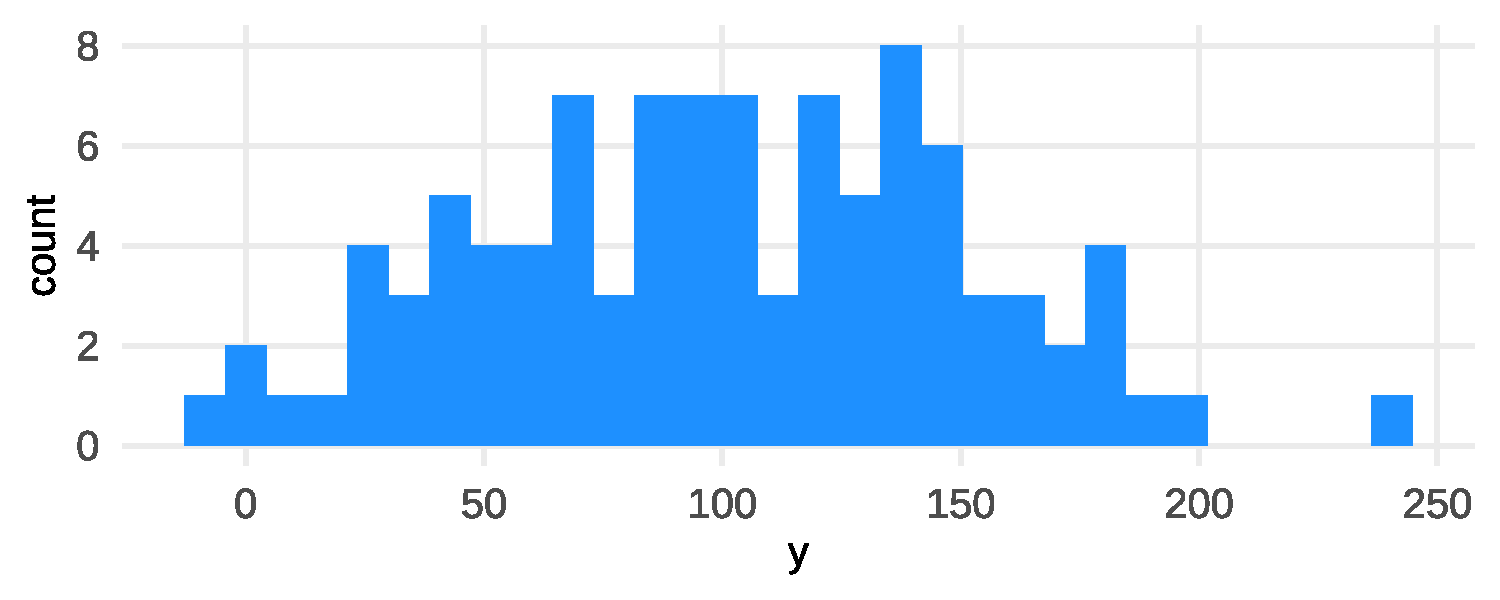
\includegraphics[keepaspectratio]{bayesian-glm_files/mediabag/bayesian-glm_files/figure-beamer/unnamed-chunk-2-1.pdf}}
\end{center}
\end{frame}

\begin{frame}[fragile]{What is a linear model?}
\phantomsection\label{what-is-a-linear-model-1}
What we can do with this variable? We can estimate the parameters that
define the Normal distribution thus \(\mu\) (the mean) and \(\sigma\)
(the standard deviation).

\begin{Shaded}
\begin{Highlighting}[]
\FunctionTok{mean}\NormalTok{(y)}
\CommentTok{\#\textgreater{} [1] 100}
\FunctionTok{sd}\NormalTok{(y)}
\CommentTok{\#\textgreater{} [1] 50}
\end{Highlighting}
\end{Shaded}
\end{frame}

\begin{frame}[fragile]{What is a linear model?}
\phantomsection\label{what-is-a-linear-model-2}
Using a linear model we can just fit a model without predictors, also
known as intercept-only model.

\begin{Shaded}
\begin{Highlighting}[]
\NormalTok{fit }\OtherTok{\textless{}{-}} \FunctionTok{glm}\NormalTok{(y }\SpecialCharTok{\textasciitilde{}} \DecValTok{1}\NormalTok{, }\AttributeTok{family =} \FunctionTok{gaussian}\NormalTok{(}\AttributeTok{link =} \StringTok{"identity"}\NormalTok{))}
\FunctionTok{summary}\NormalTok{(fit)}
\end{Highlighting}
\end{Shaded}

\begin{verbatim}
#> 
#> Call:
#> glm(formula = y ~ 1, family = gaussian(link = "identity"))
#> 
#> Coefficients:
#>             Estimate Std. Error t value Pr(>|t|)    
#> (Intercept)      100          5      20   <2e-16 ***
#> ---
#> Signif. codes:  0 '***' 0.001 '**' 0.01 '*' 0.05 '.' 0.1 ' ' 1
#> 
#> (Dispersion parameter for gaussian family taken to be 2500)
#> 
#>     Null deviance: 247500  on 99  degrees of freedom
#> Residual deviance: 247500  on 99  degrees of freedom
#> AIC: 1069.2
#> 
#> Number of Fisher Scoring iterations: 2
\end{verbatim}
\end{frame}

\begin{frame}[fragile]{What is a linear model?}
\phantomsection\label{what-is-a-linear-model-3}
I am using \texttt{glm} because I want to estimate parameters using
Maximul Likelihood, but the results are the same as using \texttt{lm}.

Basically we estimated the mean \texttt{(Intercept)} and the standard
deviation \texttt{Dispersion}, just take the square root thus 50.

What we are doing is essentially finding the \(\mu\) and \(\sigma\) that
maximised the log-likelihood of the model fixing the observed data.
\end{frame}

\begin{frame}{What is a linear model?}
\phantomsection\label{what-is-a-linear-model-4}
\begin{center}
\pandocbounded{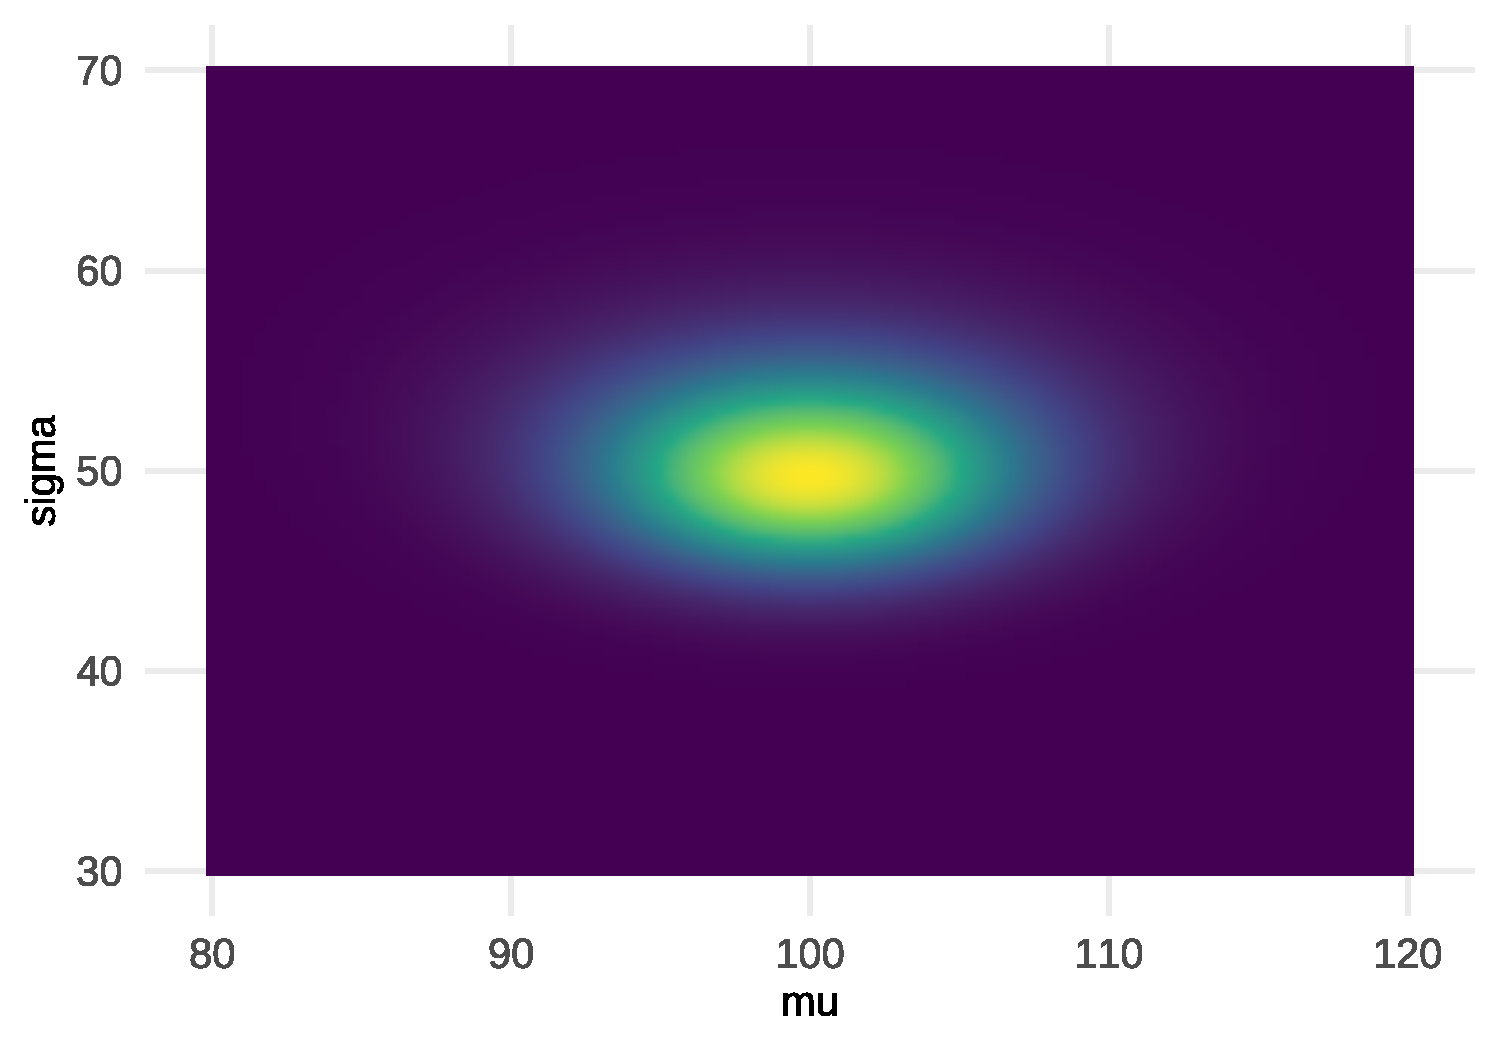
\includegraphics[keepaspectratio]{bayesian-glm_files/mediabag/bayesian-glm_files/figure-beamer/unnamed-chunk-5-1.pdf}}
\end{center}
\end{frame}

\begin{frame}{What is a linear model?}
\phantomsection\label{what-is-a-linear-model-5}
And assuming that we know \(\sigma\) (thus fixing it at 50):

\begin{center}
\pandocbounded{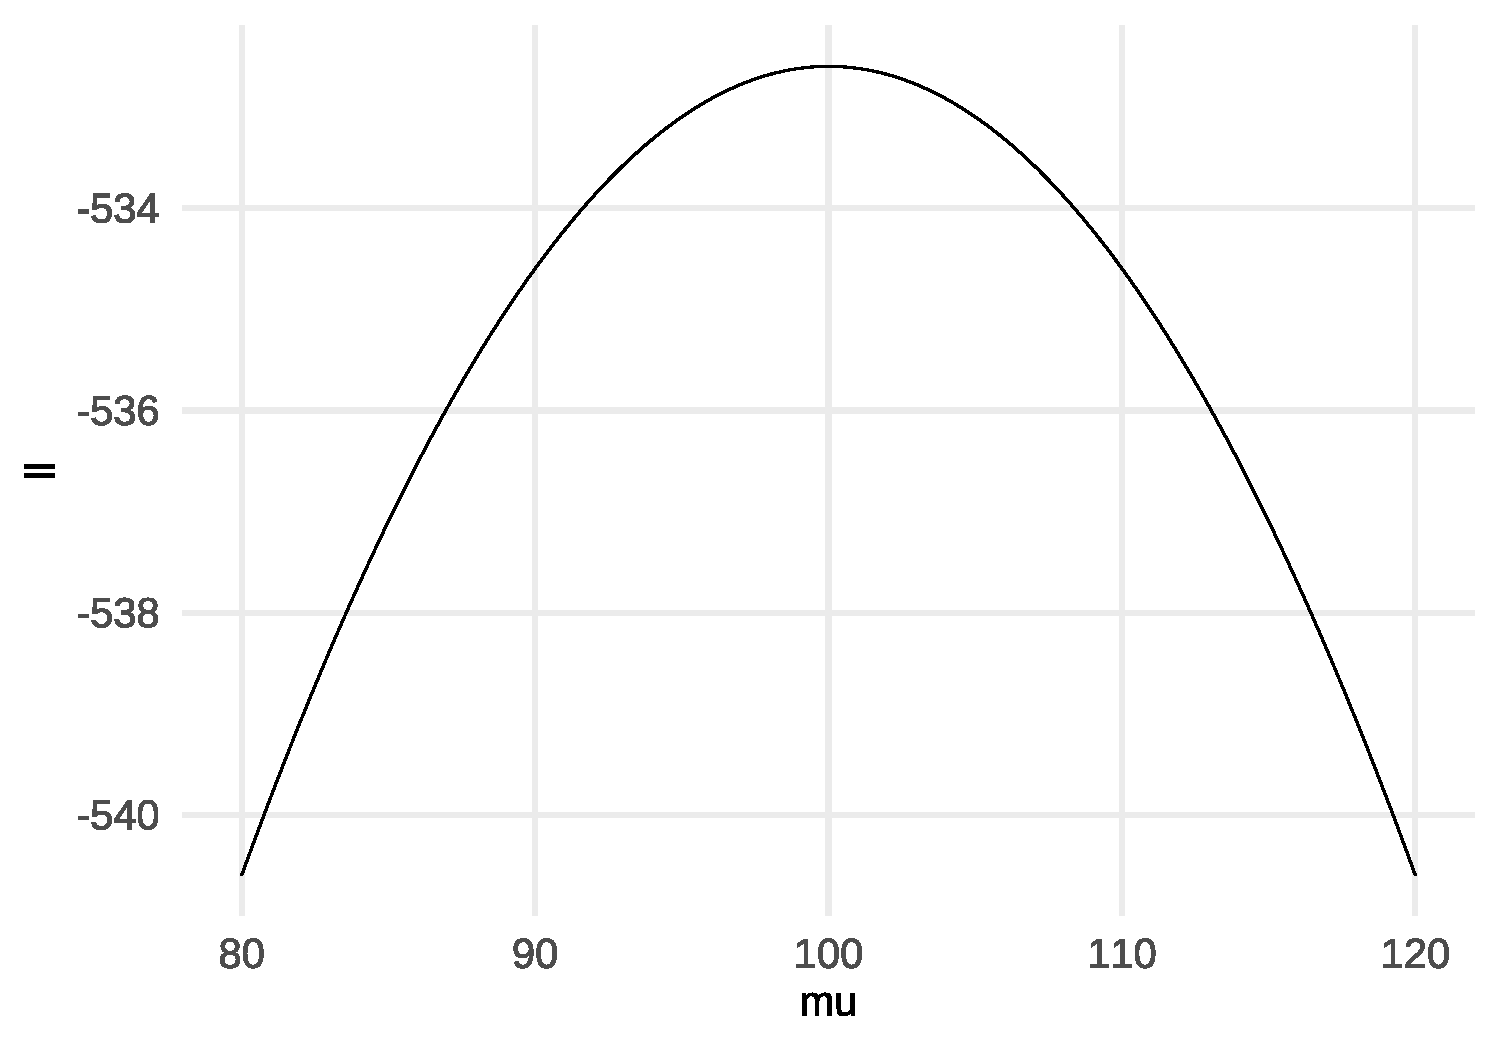
\includegraphics[keepaspectratio]{bayesian-glm_files/mediabag/bayesian-glm_files/figure-beamer/unnamed-chunk-6-1.pdf}}
\end{center}
\end{frame}

\begin{frame}[fragile]{What is a linear model?}
\phantomsection\label{what-is-a-linear-model-6}
Thus, with the estimates of \texttt{glm}, we have this model fitted on
the data:

\begin{center}
\pandocbounded{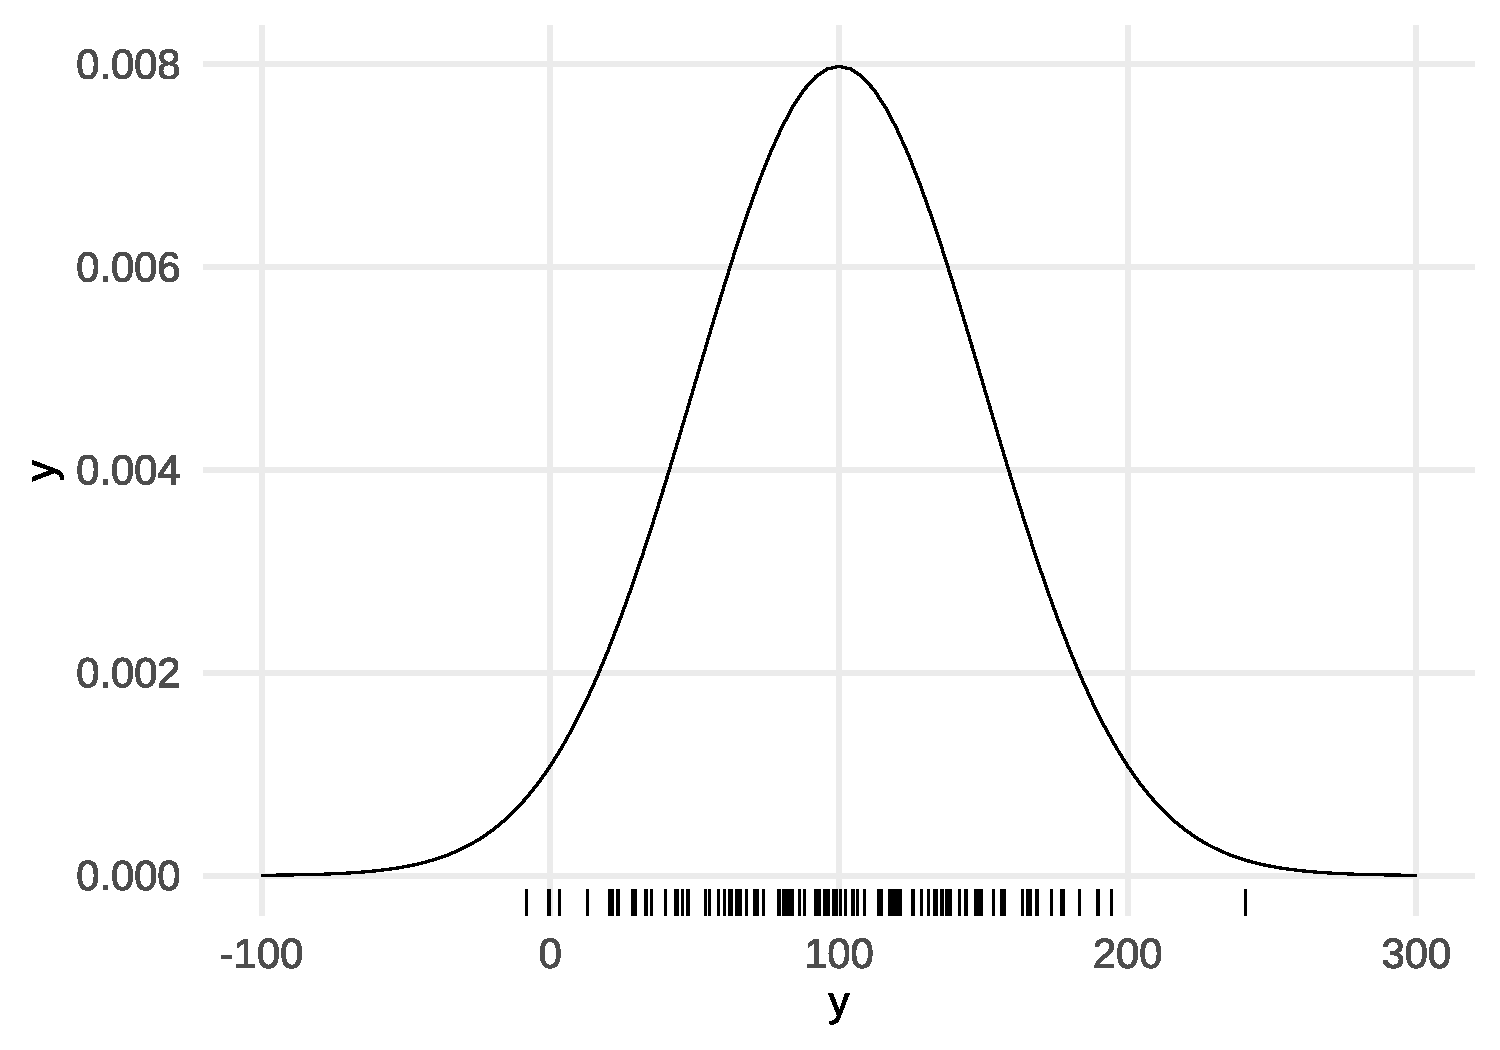
\includegraphics[keepaspectratio]{bayesian-glm_files/mediabag/bayesian-glm_files/figure-beamer/unnamed-chunk-7-1.pdf}}
\end{center}
\end{frame}

\begin{frame}[fragile]{Including a predictor}
\phantomsection\label{including-a-predictor}
When we include a predictor, we are actually try to explain the
variability of \texttt{y} using a variable \texttt{x}. For example, this
is an hypothetical relationship:

\begin{center}
\pandocbounded{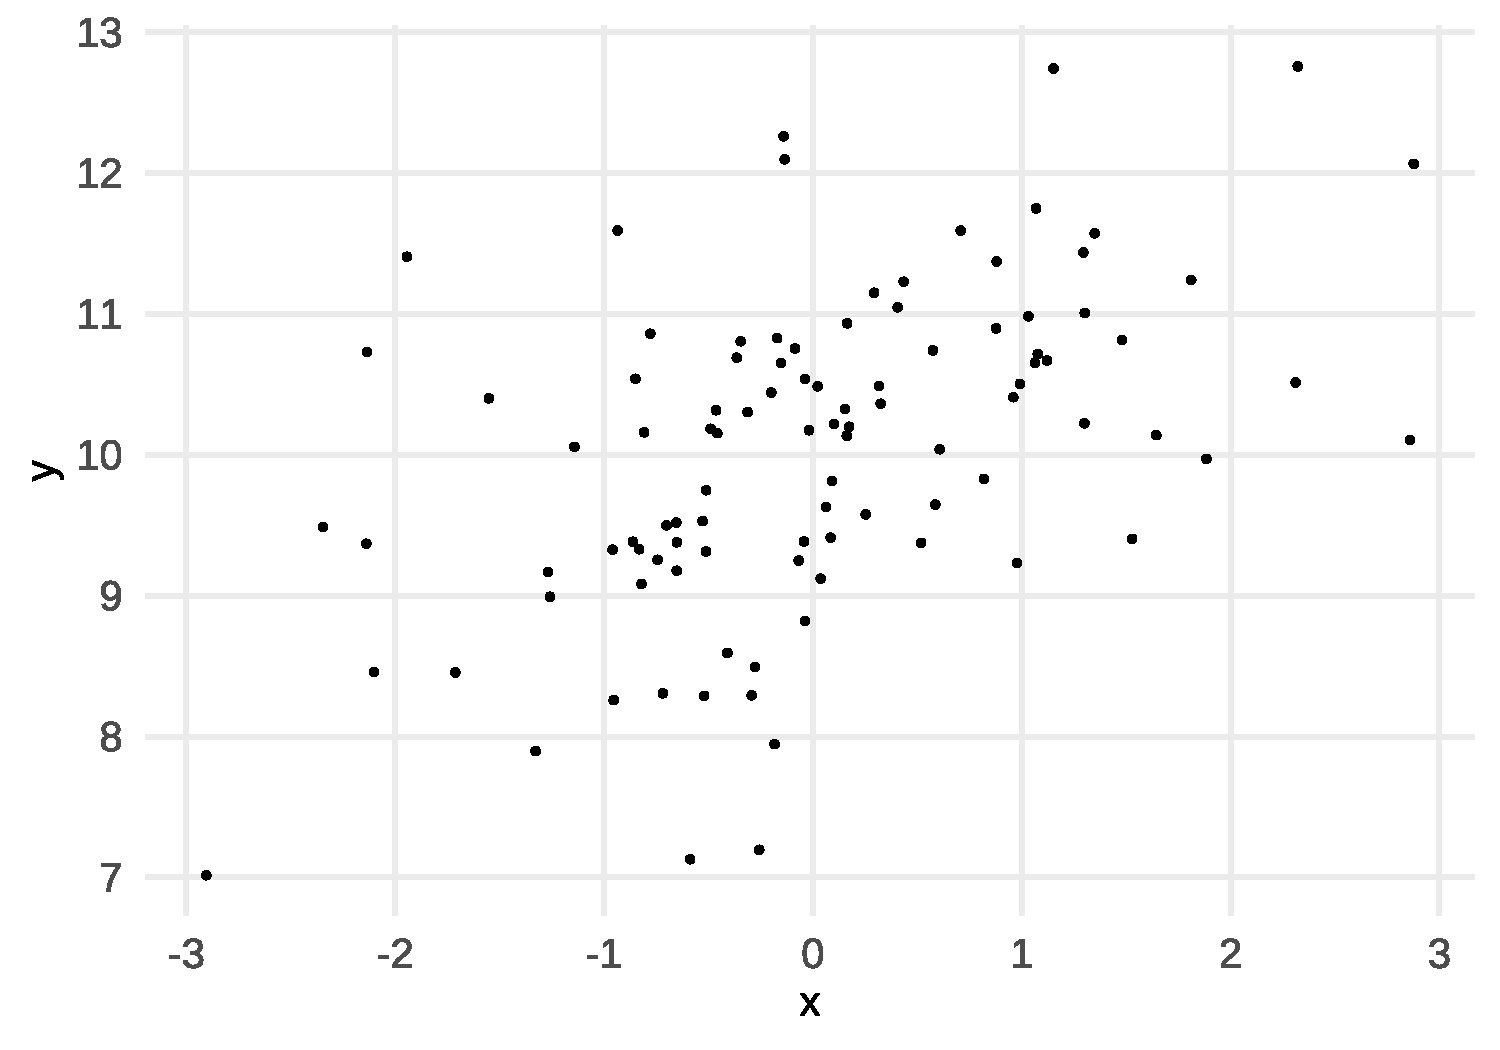
\includegraphics[keepaspectratio]{bayesian-glm_files/mediabag/bayesian-glm_files/figure-beamer/unnamed-chunk-8-1.pdf}}
\end{center}

Seems that there is a positive (linear) relationship between \texttt{x}
and \texttt{y}. We can try to improve the previous model by adding the
predictor:

\begin{Shaded}
\begin{Highlighting}[]
\NormalTok{fit }\OtherTok{\textless{}{-}} \FunctionTok{glm}\NormalTok{(y }\SpecialCharTok{\textasciitilde{}}\NormalTok{ x, }\AttributeTok{family =} \FunctionTok{gaussian}\NormalTok{(}\AttributeTok{link =} \StringTok{"identity"}\NormalTok{))}
\FunctionTok{summary}\NormalTok{(fit)}
\end{Highlighting}
\end{Shaded}

\begin{verbatim}
#> 
#> Call:
#> glm(formula = y ~ x, family = gaussian(link = "identity"))
#> 
#> Coefficients:
#>             Estimate Std. Error t value Pr(>|t|)    
#> (Intercept) 10.03509    0.10076  99.599  < 2e-16 ***
#> x            0.51628    0.09258   5.577 2.17e-07 ***
#> ---
#> Signif. codes:  0 '***' 0.001 '**' 0.01 '*' 0.05 '.' 0.1 ' ' 1
#> 
#> (Dispersion parameter for gaussian family taken to be 1.01512)
#> 
#>     Null deviance: 131.051  on 99  degrees of freedom
#> Residual deviance:  99.482  on 98  degrees of freedom
#> AIC: 289.27
#> 
#> Number of Fisher Scoring iterations: 2
\end{verbatim}

\begin{center}
\pandocbounded{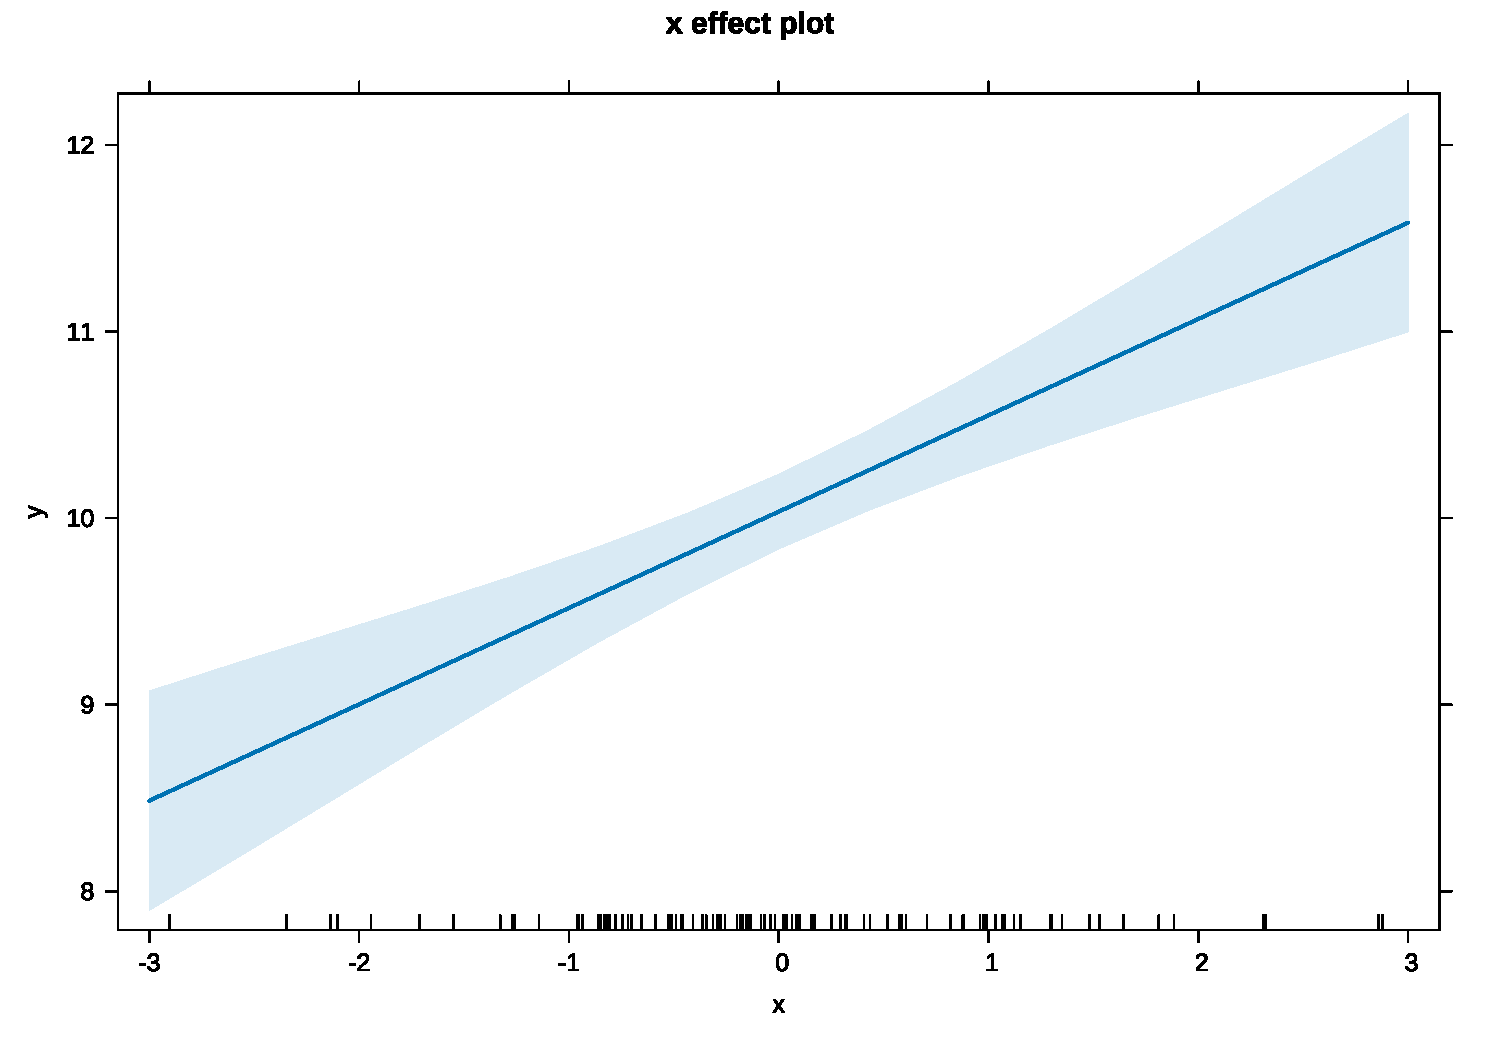
\includegraphics[keepaspectratio]{bayesian-glm_files/mediabag/bayesian-glm_files/figure-beamer/unnamed-chunk-10-1.pdf}}
\end{center}
\end{frame}

\begin{frame}[fragile]{Assumptions of the linear model}
\phantomsection\label{assumptions-of-the-linear-model}
More practicaly, we are saying that the model allows for varying the
mean i.e., each \texttt{x} value can be associated with a different
\(\mu\) but with a fixed (and estimated) \(\sigma\).

\begin{center}
\pandocbounded{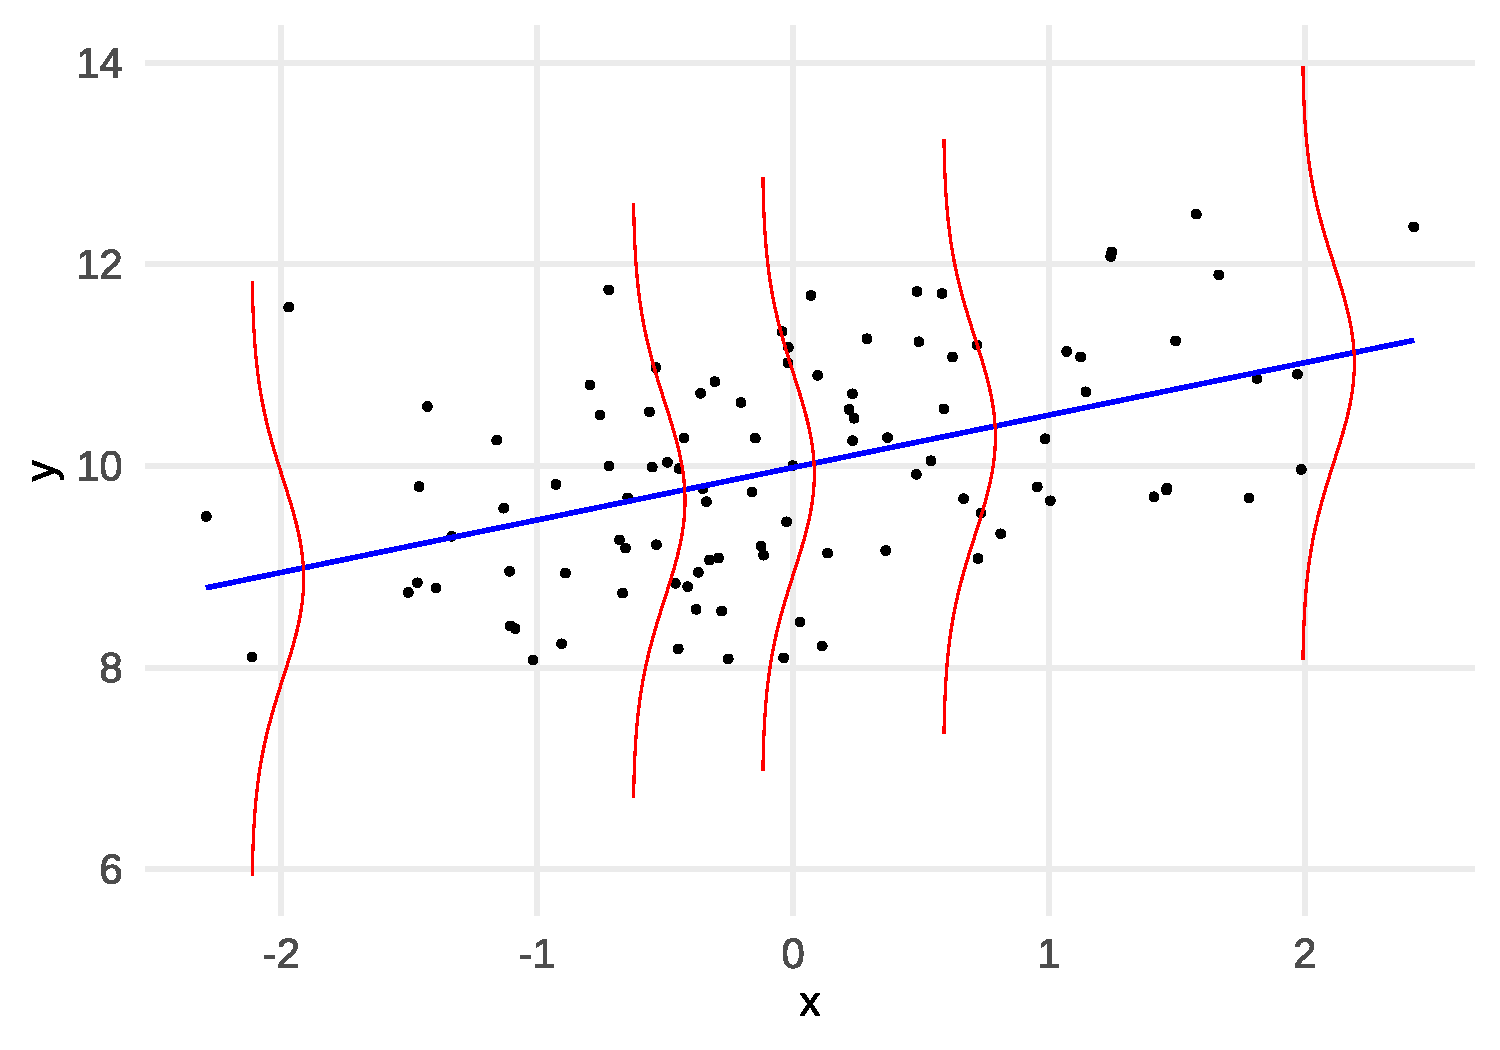
\includegraphics[keepaspectratio]{bayesian-glm_files/mediabag/bayesian-glm_files/figure-beamer/unnamed-chunk-11-1.pdf}}
\end{center}
\end{frame}

\section{Generalized linear models}\label{generalized-linear-models}

\begin{frame}{Recipe for a GLM}
\phantomsection\label{recipe-for-a-glm}
\begin{itemize}
\tightlist
\item
  \textbf{Random Component}
\item
  \textbf{Systematic Component}
\item
  \textbf{Link Function}
\end{itemize}
\end{frame}

\begin{frame}{Random Component}
\phantomsection\label{random-component}
The \textbf{random component} of a GLM identify the response variable
\(y\) coming from a certain probability distribution.

\begin{center}
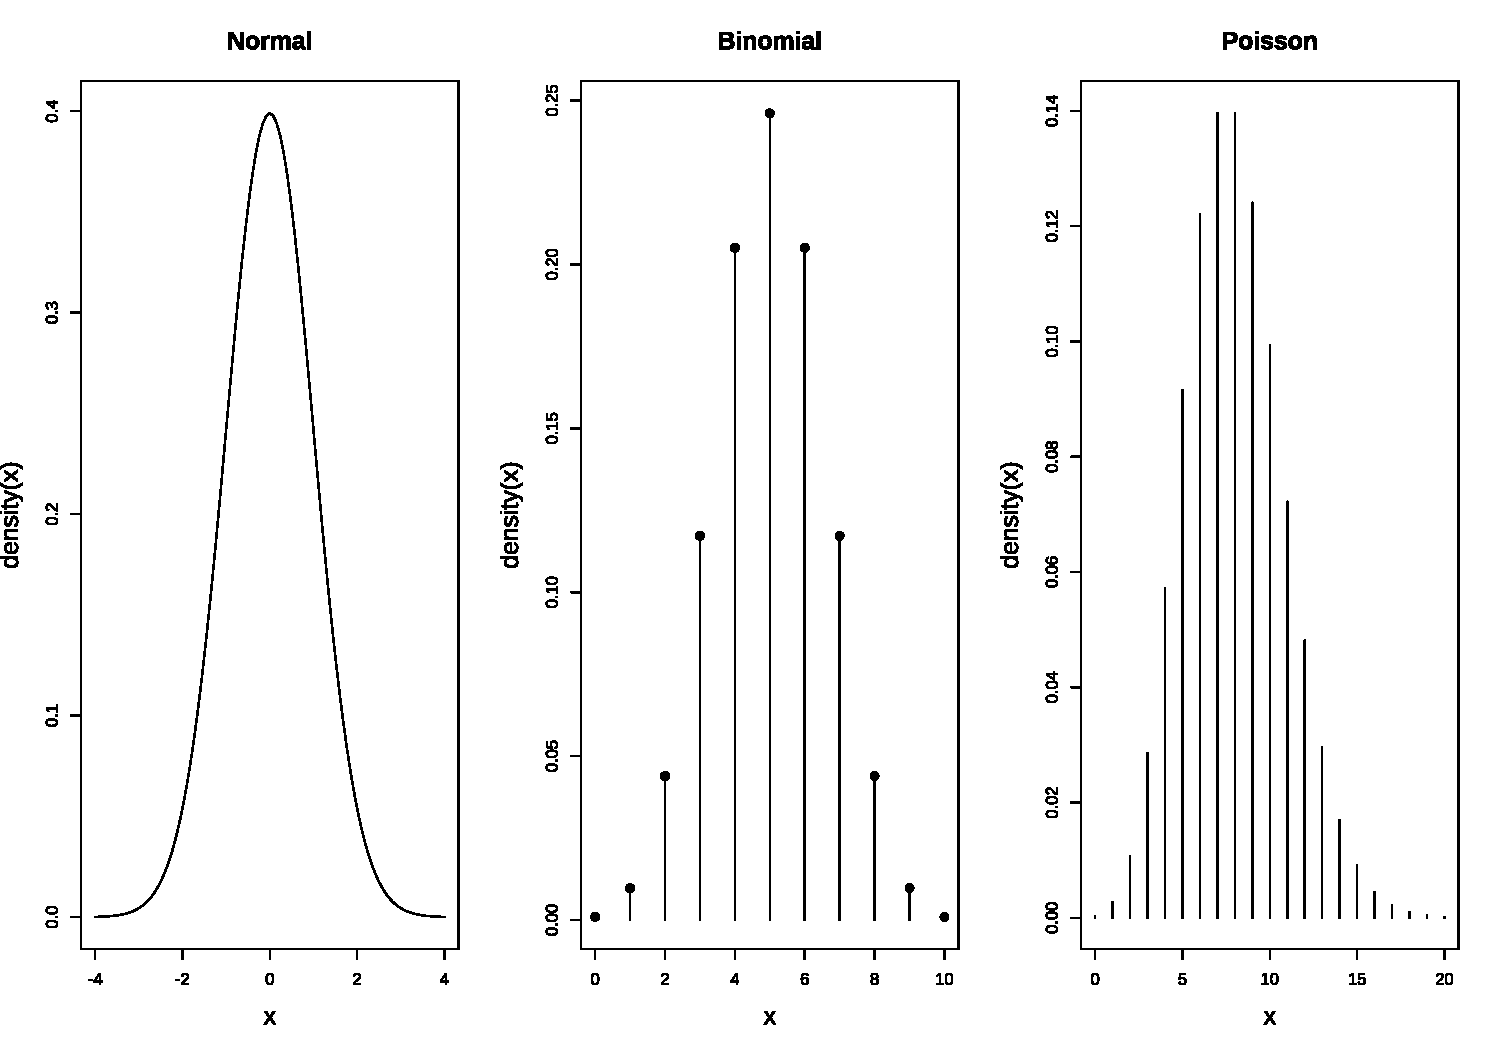
\includegraphics[width=0.5\linewidth,height=\textheight,keepaspectratio]{bayesian-glm_files/mediabag/bayesian-glm_files/figure-beamer/unnamed-chunk-12-1.pdf}
\end{center}
\end{frame}

\begin{frame}{Random Component}
\phantomsection\label{random-component-1}
\begin{itemize}
\tightlist
\item
  In practice, by definition the GLM is a model where the random
  component is a distribution of the
  \href{https://en.wikipedia.org/wiki/Exponential_family}{Exponential
  Family}. For example the Gaussian distribution, the Gamma distribution
  or the Binomial are part of the Exponential Family.
\item
  These distribution can be described using a \textbf{location}
  parameter (e.g., the mean) and a \textbf{scale} parameter (e.g., the
  variance).
\item
  The distributions are defined by parameters (e.g., \(\mu\) and
  \(\sigma\) for the Gaussian or \(\lambda\) for the Poisson). The
  location (or mean) can be directly one of the parameter or a
  combination of parameters.
\end{itemize}
\end{frame}

\begin{frame}{Random Component, Poisson example}
\phantomsection\label{random-component-poisson-example}
For example, the
\href{https://it.wikipedia.org/wiki/Distribuzione_di_Poisson}{Poisson
distribution} is defined as:

\[
f(k,\lambda) = Pr(X = k) = \frac{\lambda^k e^{-\lambda}}{k!}
\]

Where \(k\) is the number of events and \(\lambda\) (the only parameter)
is the \emph{rate}.
\end{frame}

\begin{frame}{Random Component, Poisson example}
\phantomsection\label{random-component-poisson-example-1}
The mean or location of the Poisson is \(\lambda\) and also the scale or
variance is \(\lambda\). Compared to the Gaussian, there are no two
parameters.

\begin{center}
\pandocbounded{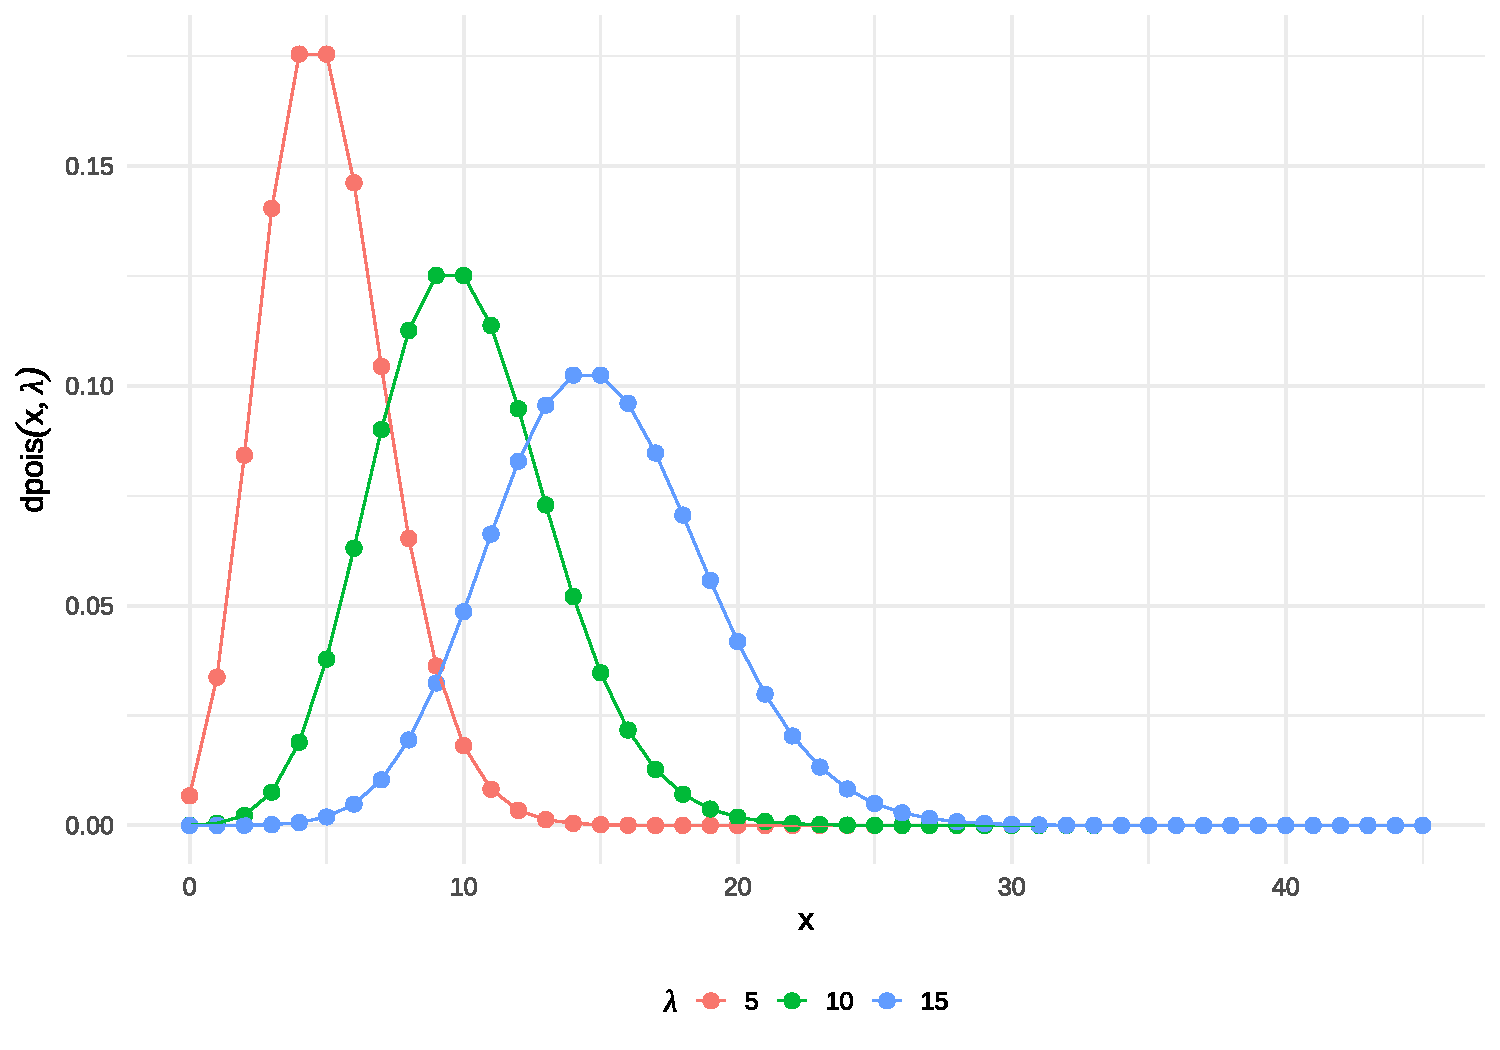
\includegraphics[keepaspectratio]{bayesian-glm_files/mediabag/bayesian-glm_files/figure-beamer/unnamed-chunk-13-1.pdf}}
\end{center}
\end{frame}

\begin{frame}{Random Component}
\phantomsection\label{random-component-2}
To sum-up, the random component represents the assumption about the
nature of our response variable. \textbf{With GLM we want to include
predictors to explain \emph{systematic} changes of the mean (but also
the scale/variance) of the random component}.

Assuming a Gaussian distribution, we try to explain how the mean of the
Gaussian distribution change according to our predictors. For the
Poisson, we include predictors on the \(\lambda\) parameters for
example.

The Random Component is called random, beacause it determines how the
\textbf{error term} \(\epsilon\) of our model is distributed.
\end{frame}

\begin{frame}{Systematic Component}
\phantomsection\label{systematic-component}
The systematic component of a GLM is the combination of predictors
(i.e., independent variables) that we want to include in the model.

The systematic component is also called \emph{linear predictor} \(\eta\)
and is usually written in equation terms as: \[
\eta_i = \beta_0 + \beta_1 x_{i1} + \beta_2 x_{i2} + \cdots + \beta_p x_{ip}
\]

Note that I am omitting the \(+ \epsilon_i\) that you usually find at
the end because this is the combination of predictors without errors.
\end{frame}

\begin{frame}{Systematic Component, an example}
\phantomsection\label{systematic-component-an-example}
Assuming that we have two groups and we want to see if there are
differences in a depression score. This is a t-test, or better a linear
model, or better a GLM.

Ignoring the random component, we can have a systematic component
written in this way:

\[
\eta_i = \beta_0 + \beta_1{\mbox{group}_i}
\]

Assuming that the group is dummy-coded, \(\beta_0\) is the mean of the
first group and \(\beta_1\) is the difference between the two groups. In
other terms, these are the true or estimated values without the error
(i.e., the random component).
\end{frame}

\begin{frame}{Systematic Component, an example}
\phantomsection\label{systematic-component-an-example-1}
Another example, assuming we have the same depression score and we want
to predict it with an anxiety score. The blue line is the true/estimated
regression line where \(\eta_i\) is the expected value for the
observation \(x_i\). The red segments are the errors or residuals i.e.,
the random component.

\begin{center}
\pandocbounded{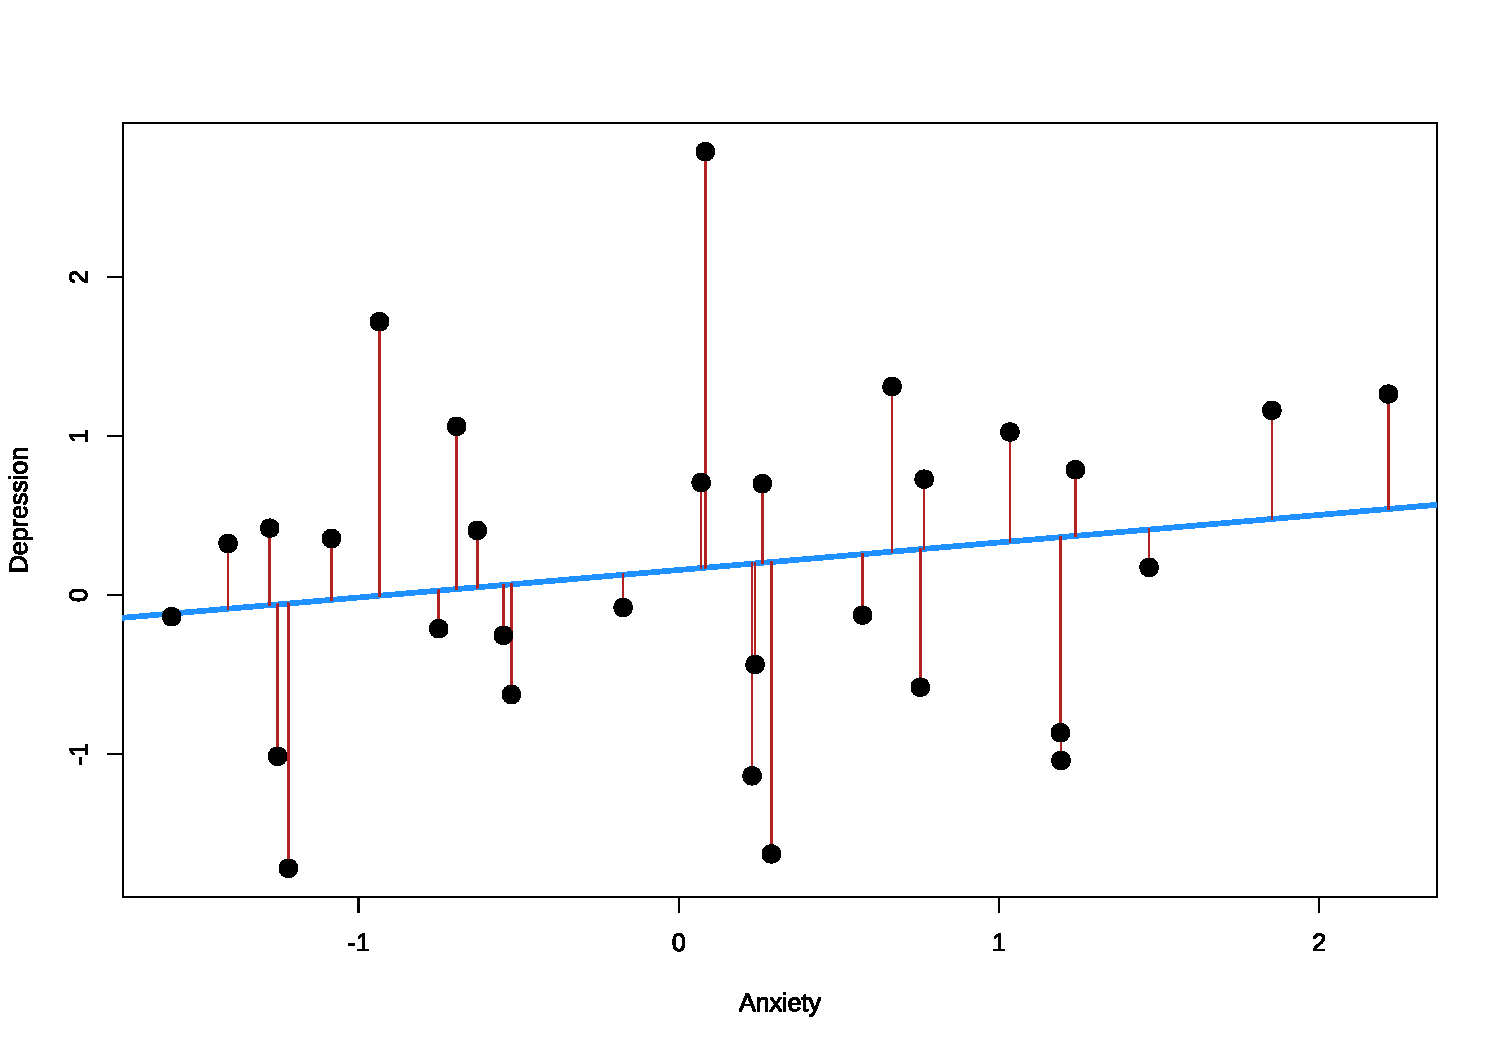
\includegraphics[keepaspectratio]{bayesian-glm_files/mediabag/bayesian-glm_files/figure-beamer/unnamed-chunk-14-1.pdf}}
\end{center}
\end{frame}

\begin{frame}{Systematic Component}
\phantomsection\label{systematic-component-1}
To sum-up, the systematic component is the combination of predictors
that are used to predict the mean of the distribution that is used as
random component. The errors part of the model is distributed as the
random component.
\end{frame}

\begin{frame}{Link Function}
\phantomsection\label{link-function}
The final element is the \textbf{link function}. The idea is that we
need a way to connect the systematic component \(\eta\) to the random
component mean \(\mu\).

The \textbf{link function} \(g(\mu)\) is an \textbf{invertible} function
that connects the mean \(\mu\) of the random component with the
\emph{linear combination} of predictors.

Thus \(\eta_i = g(\mu_i)\) and \(\mu_i = g(\eta_i)^{-1}\). The
systematic component is not affected by \(g()\) while the relationship
between \(\mu\) and \(\eta\) changes using different link functions.

\[
g(\mu_i) = \eta_i = \beta_0 + \beta_1 x_{i1} + \beta_2 x_{i2} + \cdots + \beta_p x_{ip}
\]

\[
\mu_i = g(\eta_i)^{-1} = \eta_i = \beta_0 + \beta_1 x_{i1} + \beta_2 x_{i2} + \cdots + \beta_p x_{ip}
\]
\end{frame}

\begin{frame}{Link function}
\phantomsection\label{link-function-1}
The simplest \textbf{link function} is the \textbf{identity link} where
\(g(\mu) = \mu\) and correspond to the standard linear model. In fact,
the linear regression is just a GLM with a \textbf{Gaussian random
component} and the \textbf{identity} link function.

\begin{table}
\caption{Main distributions and link functions}\tabularnewline

\fontsize{12.0pt}{14.4pt}\selectfont
\begin{tabular*}{\linewidth}{@{\extracolsep{\fill}}ccc}
\toprule
{\bfseries Family} & {\bfseries Link} & {\bfseries Range} \\ 
\midrule\addlinespace[2.5pt]
\texttt{gaussian} & identity & $$(-\infty,+\infty)$$ \\ 
\texttt{gamma} & log & $$(0,+\infty)$$ \\ 
\texttt{binomial} & logit & $$\frac{0, 1, ..., n_{i}}{n_{i}}$$ \\ 
\texttt{binomial} & probit & $$\frac{0, 1, ..., n_{i}}{n_{i}}$$ \\ 
\texttt{poisson} & log & $$0, 1, 2, ...$$ \\ 
\bottomrule
\end{tabular*}
\end{table}
\end{frame}

\begin{frame}[fragile]{Gaussian GLM}
\phantomsection\label{gaussian-glm}
Thus remember that when you do a \texttt{lm} or \texttt{lmer} you are
actually doing a GLM with a Gaussian random component and an identity
link function. You are including predictors (systematic component)
explaining changes in the mean of the Gaussian distribution.

\begin{columns}[T]
\begin{column}{0.48\linewidth}
\begin{Shaded}
\begin{Highlighting}[]
\FunctionTok{lm}\NormalTok{(y }\SpecialCharTok{\textasciitilde{}}\NormalTok{ x)}
\end{Highlighting}
\end{Shaded}

\begin{verbatim}
#> 
#> Call:
#> lm(formula = y ~ x)
#> 
#> Coefficients:
#> (Intercept)            x  
#>      0.3386       0.5278
\end{verbatim}
\end{column}

\begin{column}{0.48\linewidth}
\begin{Shaded}
\begin{Highlighting}[]
\FunctionTok{glm}\NormalTok{(y }\SpecialCharTok{\textasciitilde{}}\NormalTok{ x, }\AttributeTok{family =} \FunctionTok{gaussian}\NormalTok{(}\AttributeTok{link =} \StringTok{"identity"}\NormalTok{))}
\end{Highlighting}
\end{Shaded}

\begin{verbatim}
#> 
#> Call:  glm(formula = y ~ x, family = gaussian(link = "identity"))
#> 
#> Coefficients:
#> (Intercept)            x  
#>      0.3386       0.5278  
#> 
#> Degrees of Freedom: 99 Total (i.e. Null);  98 Residual
#> Null Deviance:       127.7 
#> Residual Deviance: 106   AIC: 295.6
\end{verbatim}
\end{column}
\end{columns}
\end{frame}

\begin{frame}[fragile]{Gaussian GLM, a simple simulation}
\phantomsection\label{gaussian-glm-a-simple-simulation}
We can understand the GLM recipe trying to simulate a simple model.
Let's simulate a relationship between two numerical variables (like the
depression and anxiety example).

\begin{Shaded}
\begin{Highlighting}[]
\NormalTok{N }\OtherTok{\textless{}{-}} \DecValTok{20}
\NormalTok{anxiety }\OtherTok{\textless{}{-}} \FunctionTok{rnorm}\NormalTok{(N, }\DecValTok{0}\NormalTok{, }\DecValTok{1}\NormalTok{) }\CommentTok{\# anxiety scores}
\NormalTok{b0 }\OtherTok{\textless{}{-}} \FloatTok{0.3} \CommentTok{\# intercept, depression when anxiety = 0}
\NormalTok{b1 }\OtherTok{\textless{}{-}} \FloatTok{0.5} \CommentTok{\# increase in depression for 1 increase in anxiety}

\CommentTok{\# systematic component}
\NormalTok{eta }\OtherTok{\textless{}{-}}\NormalTok{ b0 }\SpecialCharTok{+}\NormalTok{ b1 }\SpecialCharTok{*}\NormalTok{ anxiety}

\NormalTok{dat }\OtherTok{\textless{}{-}} \FunctionTok{data.frame}\NormalTok{(anxiety, b0, b1, eta)}
\FunctionTok{head}\NormalTok{(dat)}
\end{Highlighting}
\end{Shaded}

\begin{verbatim}
#>      anxiety  b0  b1         eta
#> 1 -0.7721991 0.3 0.5 -0.08609956
#> 2 -1.7673666 0.3 0.5 -0.58368331
#> 3 -2.4591603 0.3 0.5 -0.92958017
#> 4 -1.5541557 0.3 0.5 -0.47707787
#> 5  1.4506526 0.3 0.5  1.02532628
#> 6 -0.1205410 0.3 0.5  0.23972952
\end{verbatim}
\end{frame}

\begin{frame}[fragile]{Gaussian GLM, a simple simulation}
\phantomsection\label{gaussian-glm-a-simple-simulation-1}
\texttt{eta} is the linear predictor (without errors):

\begin{center}
\pandocbounded{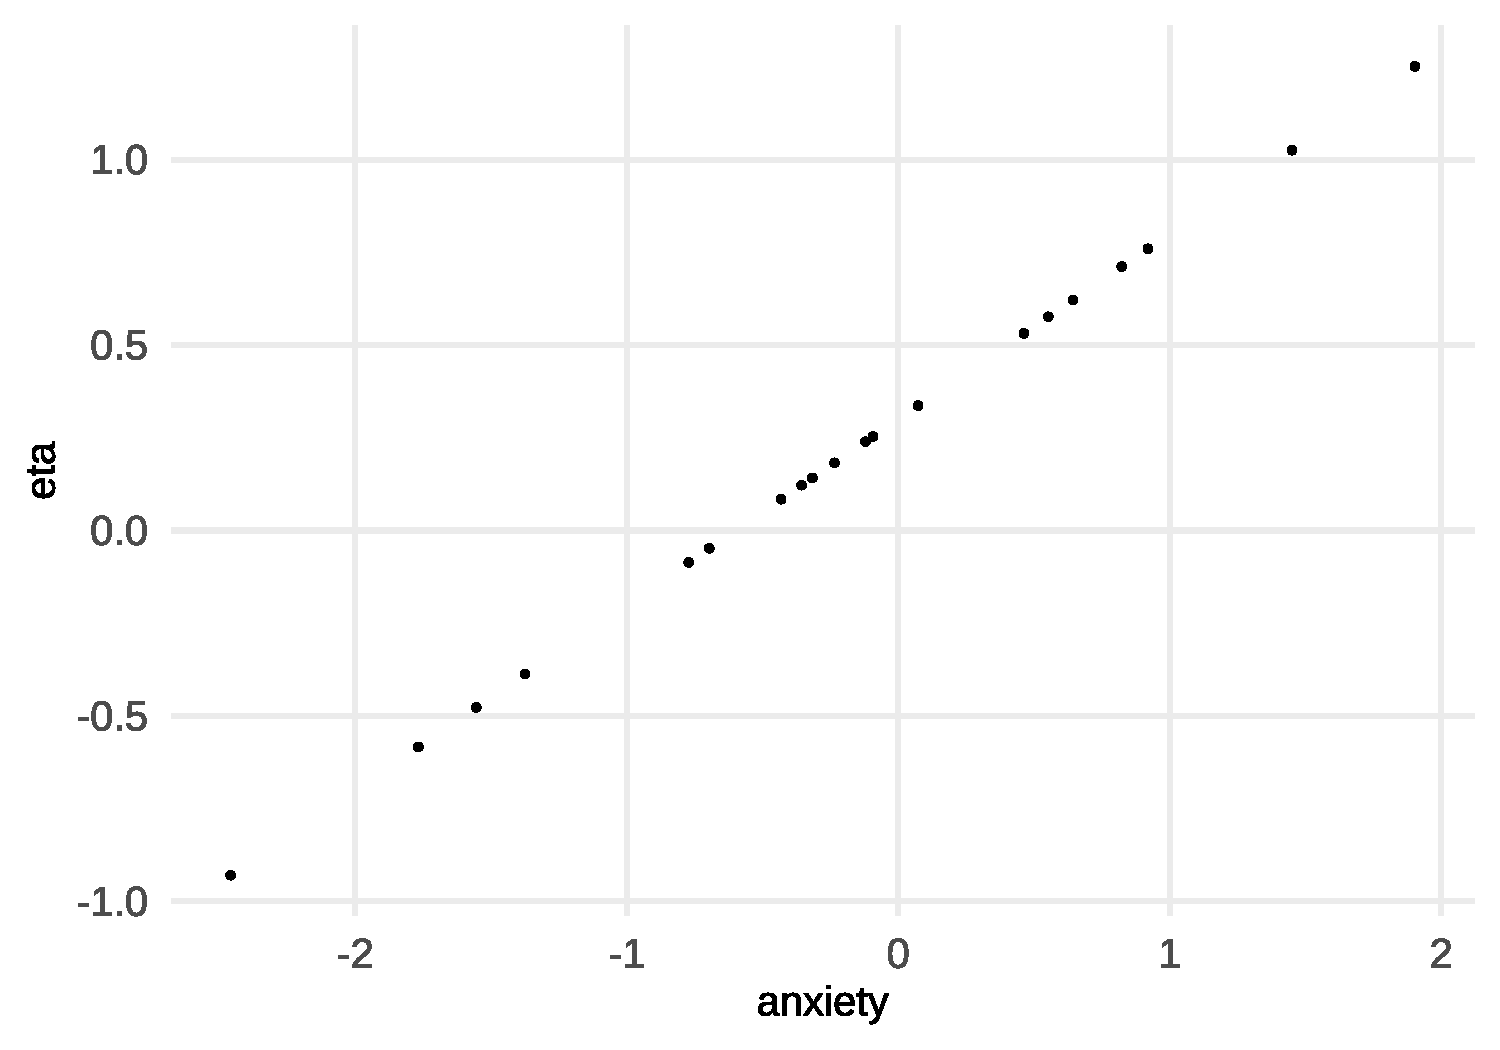
\includegraphics[keepaspectratio]{bayesian-glm_files/mediabag/bayesian-glm_files/figure-beamer/unnamed-chunk-20-1.pdf}}
\end{center}

Thus the expected value of a person with \(\mbox{anxiety} = -1\) is
\(\beta_0 + \beta_1\times(-1)\) thus -0.2.
\end{frame}

\begin{frame}[fragile]{Gaussian GLM, a simple simulation}
\phantomsection\label{gaussian-glm-a-simple-simulation-2}
Now, for a realistic simulation we need some random errors. The random
component here is a Gaussian distribution thus each observed (or
simulated) value is the systematic component plus the random error
\(\mbox{depression}_i = \eta_i + \epsilon_i\).

The errors (or residuals) are assumed to be normally distributed with
\(\mu = 0\) and variance \(\sigma^2_{\epsilon}\) (the residual standard
deviation).

\begin{Shaded}
\begin{Highlighting}[]
\NormalTok{sigma }\OtherTok{\textless{}{-}} \DecValTok{1} \CommentTok{\# residual standard deviation}
\NormalTok{error }\OtherTok{\textless{}{-}} \FunctionTok{rnorm}\NormalTok{(N, }\DecValTok{0}\NormalTok{, sigma)}
\NormalTok{depression }\OtherTok{\textless{}{-}}\NormalTok{ eta }\SpecialCharTok{+}\NormalTok{ error }\CommentTok{\# b0 + b1 * anxiety + error}
\end{Highlighting}
\end{Shaded}
\end{frame}

\begin{frame}{Gaussian GLM, a simple simulation}
\phantomsection\label{gaussian-glm-a-simple-simulation-3}
This is the simulated dataset. The blue line is the linear predictor and
the red segments are the Gaussian residuals.

\begin{center}
\pandocbounded{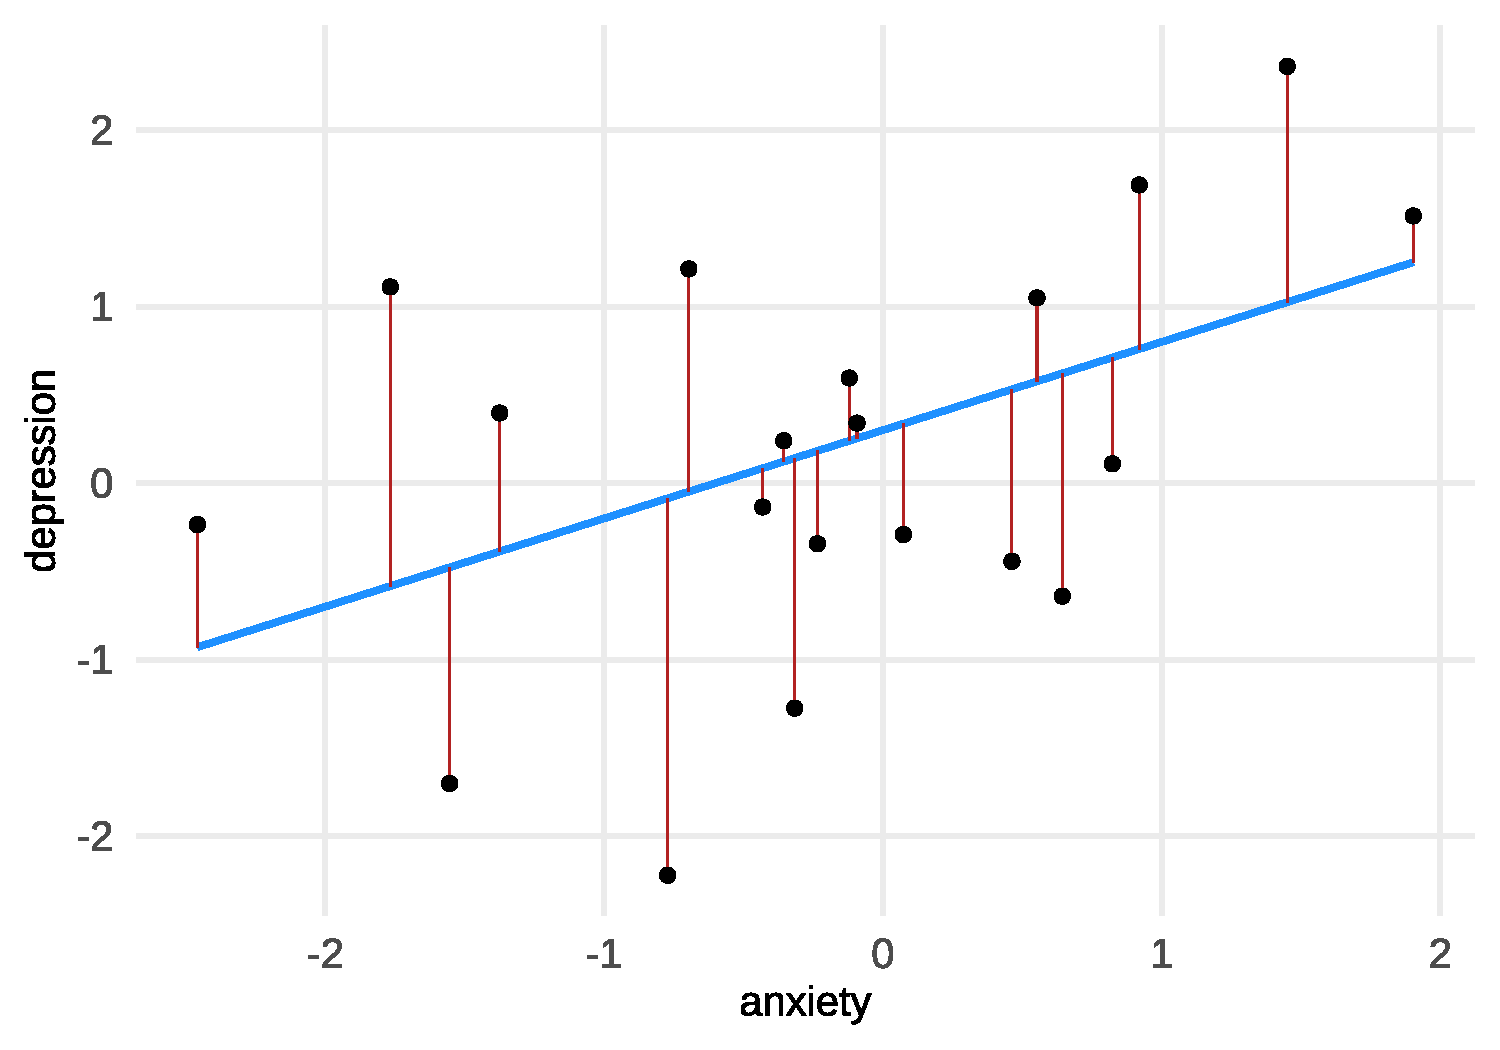
\includegraphics[keepaspectratio]{bayesian-glm_files/mediabag/bayesian-glm_files/figure-beamer/unnamed-chunk-22-1.pdf}}
\end{center}
\end{frame}

\begin{frame}{Gaussian GLM, a simple simulation}
\phantomsection\label{gaussian-glm-a-simple-simulation-4}
If we plot the red segments we have roughly a Gaussian distribution.
This is the assumption of the GLM with a Gaussian random component.

\begin{center}
\pandocbounded{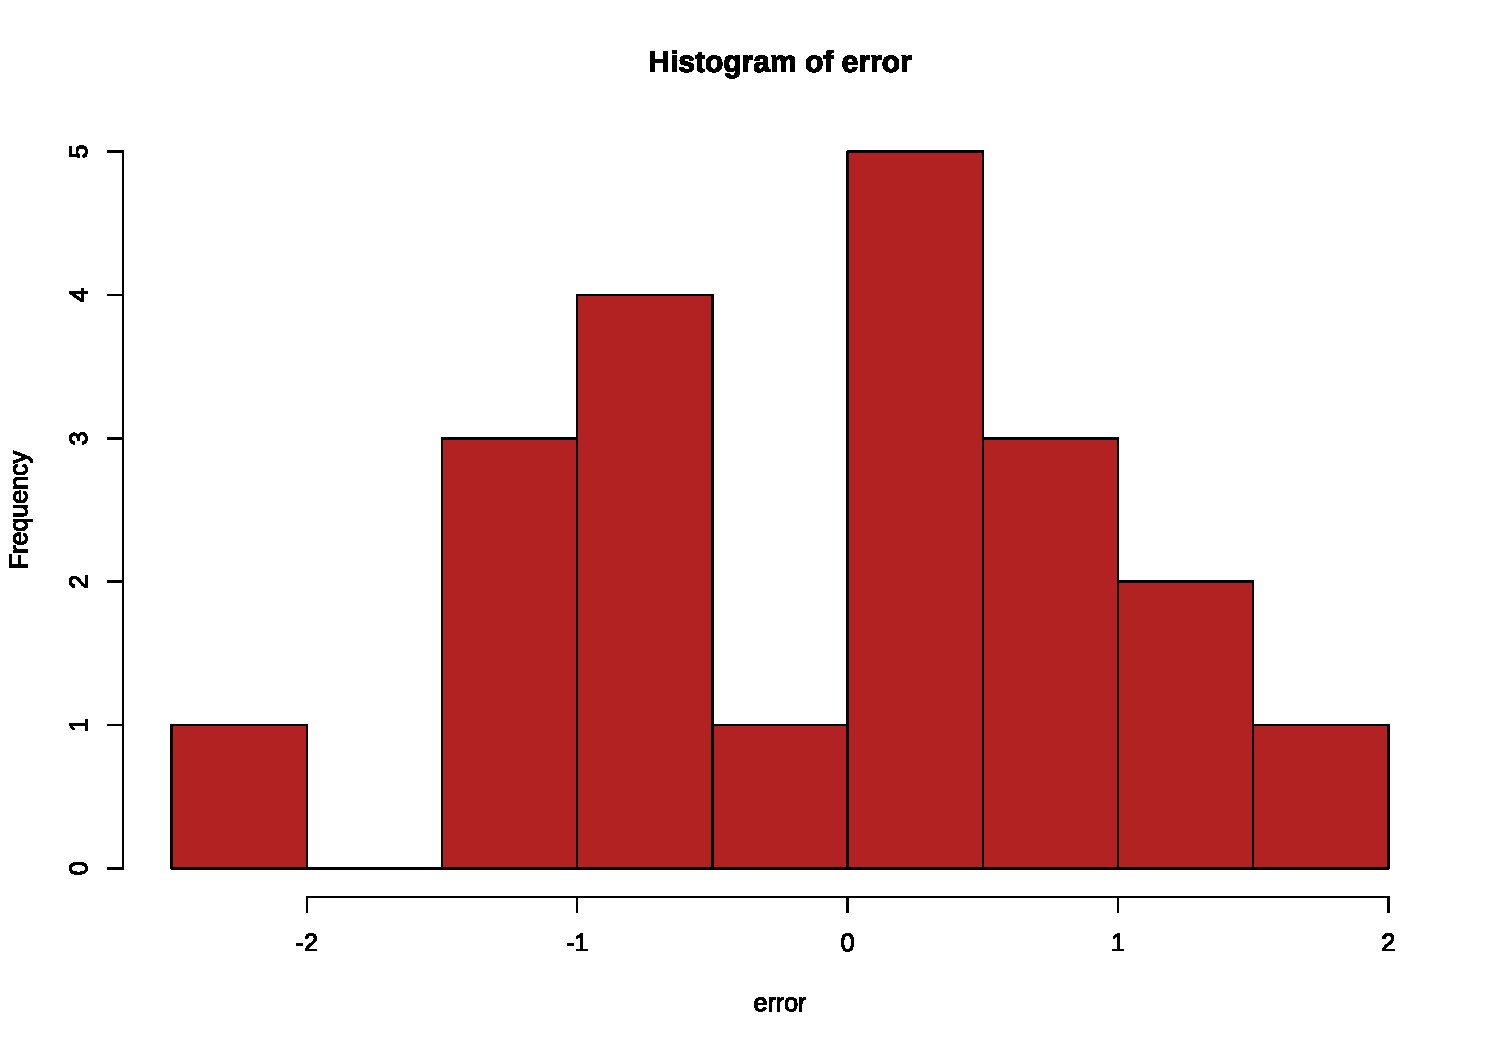
\includegraphics[keepaspectratio]{bayesian-glm_files/mediabag/bayesian-glm_files/figure-beamer/unnamed-chunk-23-1.pdf}}
\end{center}
\end{frame}

\begin{frame}[fragile]{What about the link function?}
\phantomsection\label{what-about-the-link-function}
The link function for the Gaussian GLM is by default the
\emph{identity}. Identity means that \(\eta_i = \mu_i\), thus there is
no transformation. Within each distribution object in R there is the
link function and the inverse:

\begin{Shaded}
\begin{Highlighting}[]
\CommentTok{\# this is the family (or random component) and the link function. doing a lm() is like glm(family = gaussian(link = "identity"))}
\NormalTok{fam }\OtherTok{\textless{}{-}} \FunctionTok{gaussian}\NormalTok{(}\AttributeTok{link =} \StringTok{"identity"}\NormalTok{)}
\NormalTok{fam}\SpecialCharTok{$}\NormalTok{linkfun }\CommentTok{\# link function specifed above}
\end{Highlighting}
\end{Shaded}

\begin{verbatim}
#> function (mu) 
#> mu
#> <environment: namespace:stats>
\end{verbatim}

\begin{Shaded}
\begin{Highlighting}[]
\NormalTok{fam}\SpecialCharTok{$}\NormalTok{linkinv }\CommentTok{\# inverse link function}
\end{Highlighting}
\end{Shaded}

\begin{verbatim}
#> function (eta) 
#> eta
#> <environment: namespace:stats>
\end{verbatim}
\end{frame}

\begin{frame}[fragile]{What about the link function?}
\phantomsection\label{what-about-the-link-function-1}
With the identity, the link function has no effect.

\begin{Shaded}
\begin{Highlighting}[]
\NormalTok{mu }\OtherTok{\textless{}{-}}\NormalTok{ fam}\SpecialCharTok{$}\FunctionTok{linkinv}\NormalTok{(b0 }\SpecialCharTok{+}\NormalTok{ b1 }\SpecialCharTok{*}\NormalTok{ anxiety)}
\FunctionTok{head}\NormalTok{(mu)}
\end{Highlighting}
\end{Shaded}

\begin{verbatim}
#> [1] -0.08609956 -0.58368331 -0.92958017 -0.47707787  1.02532628  0.23972952
\end{verbatim}

\begin{Shaded}
\begin{Highlighting}[]
\FunctionTok{head}\NormalTok{(fam}\SpecialCharTok{$}\FunctionTok{linkfun}\NormalTok{(mu))}
\end{Highlighting}
\end{Shaded}

\begin{verbatim}
#> [1] -0.08609956 -0.58368331 -0.92958017 -0.47707787  1.02532628  0.23972952
\end{verbatim}

But with other GLMs, (e.g., logistic regression) the link function is
the core element.
\end{frame}

\begin{frame}[fragile]{Gaussian GLM, a simple simulation}
\phantomsection\label{gaussian-glm-a-simple-simulation-5}
A more compact (and useful) way to simulate the data is:

\begin{Shaded}
\begin{Highlighting}[]
\NormalTok{depression }\OtherTok{\textless{}{-}} \FunctionTok{rnorm}\NormalTok{(N, }\AttributeTok{mean =}\NormalTok{ fam}\SpecialCharTok{$}\FunctionTok{linkinv}\NormalTok{(b0 }\SpecialCharTok{+}\NormalTok{ b1 }\SpecialCharTok{*}\NormalTok{ anxiety), }\AttributeTok{sd =}\NormalTok{ sigma)}
\end{Highlighting}
\end{Shaded}

In this way is more clear that we are generating data from a normal
distribution with fixed \(\sigma^2_{\epsilon}\) and we are modeling the
mean.
\end{frame}

\section{Parameters intepretation}\label{parameters-intepretation}

\begin{frame}[fragile]{Parameters intepretation}
\phantomsection\label{parameters-intepretation-1}
Let's make a more complex example with a Gaussian GLM with more than one
predictor. We have a dataset with 150 observations and some variables.

\begin{verbatim}
#>   depression age group    anxiety
#> 1 -0.2173456  23    g1  0.0022093
#> 2  0.3273544  40    g2 -0.1100926
#> 3  1.0405812  24    g1  0.4261357
#> 4  2.8139121  33    g2  1.8146185
#> 5  0.7347837  30    g1 -0.1817395
#> 6  0.6209260  26    g2 -1.2488724
\end{verbatim}

We want to predict the \texttt{depression} with \texttt{anxiety},
\texttt{group} and \texttt{age}.
\end{frame}

\begin{frame}[fragile]{Parameters intepretation}
\phantomsection\label{parameters-intepretation-2}
Let's fit the model (here using \texttt{lm} but is a GLM!):

\begin{verbatim}
#> 
#> Call:
#> lm(formula = depression ~ anxiety + group + age, data = dat)
#> 
#> Residuals:
#>     Min      1Q  Median      3Q     Max 
#> -2.0837 -0.6937 -0.1653  0.5869  3.1663 
#> 
#> Coefficients:
#>              Estimate Std. Error t value Pr(>|t|)    
#> (Intercept) -0.229923   0.326055  -0.705  0.48183    
#> anxiety      0.526979   0.081160   6.493 1.23e-09 ***
#> groupg2      0.367025   0.165569   2.217  0.02819 *  
#> age          0.024005   0.009075   2.645  0.00906 ** 
#> ---
#> Signif. codes:  0 '***' 0.001 '**' 0.01 '*' 0.05 '.' 0.1 ' ' 1
#> 
#> Residual standard error: 1.013 on 146 degrees of freedom
#> Multiple R-squared:  0.2574, Adjusted R-squared:  0.2421 
#> F-statistic: 16.87 on 3 and 146 DF,  p-value: 1.844e-09
\end{verbatim}

How do you intepret the output? and the model parameters?
\end{frame}

\section{Bayesian Models}\label{bayesian-models}

\begin{frame}{Bayesian vs Frequentists GLM}
\phantomsection\label{bayesian-vs-frequentists-glm}
What about the Bayesian version of the previous model? Actually the main
difference is that we need to include the priors to obtain posterior
distributions about model parameters. The likelihood part is extactly
the same as non-bayesian models.
\end{frame}

\begin{frame}[fragile]{\texttt{brms}}
\phantomsection\label{brms}
There are several R packages for estimating Bayesian GLMs. The most
complete is called \href{https://paulbuerkner.com/brms/}{\texttt{brms}}.

There are also other options such as \texttt{rstanarm}.
\texttt{rstanarm} is faster but less flexible. \texttt{brms} include all
GLMs (and also other models such as meta-analysis, multivariate, etc.)
but is slower and requires more knowledge.

The syntax is the same as \texttt{lm} or \texttt{glm} and also
\texttt{lme4} if you want to include random-effects.
\end{frame}

\begin{frame}[fragile]{\texttt{brms}}
\phantomsection\label{brms-1}
Let's start with a simple model, predicting the \texttt{depression} with
the group. Thus essentially a t-test:

\begin{Shaded}
\begin{Highlighting}[]
\NormalTok{fit\_group }\OtherTok{\textless{}{-}} \FunctionTok{brm}\NormalTok{(depression }\SpecialCharTok{\textasciitilde{}}\NormalTok{ group, }
                 \AttributeTok{data =}\NormalTok{ dat, }
                 \AttributeTok{family =} \FunctionTok{gaussian}\NormalTok{(}\AttributeTok{link =} \StringTok{"identity"}\NormalTok{), }
                 \AttributeTok{file =} \FunctionTok{here}\NormalTok{(}\StringTok{"slides/objects/fit\_group.rds"}\NormalTok{))}
\end{Highlighting}
\end{Shaded}
\end{frame}

\begin{frame}[fragile]{\texttt{brms}}
\phantomsection\label{brms-2}
\begin{Shaded}
\begin{Highlighting}[]
\FunctionTok{summary}\NormalTok{(fit\_group)}
\end{Highlighting}
\end{Shaded}

\begin{verbatim}
#>  Family: gaussian 
#>   Links: mu = identity; sigma = identity 
#> Formula: depression ~ group 
#>    Data: dat (Number of observations: 150) 
#>   Draws: 4 chains, each with iter = 2000; warmup = 1000; thin = 1;
#>          total post-warmup draws = 4000
#> 
#> Regression Coefficients:
#>           Estimate Est.Error l-95% CI u-95% CI Rhat Bulk_ESS Tail_ESS
#> Intercept     0.56      0.13     0.31     0.82 1.00     3601     2924
#> groupg2       0.44      0.18     0.08     0.80 1.00     3456     2832
#> 
#> Further Distributional Parameters:
#>       Estimate Est.Error l-95% CI u-95% CI Rhat Bulk_ESS Tail_ESS
#> sigma     1.11      0.07     1.00     1.26 1.00     3865     2502
#> 
#> Draws were sampled using sampling(NUTS). For each parameter, Bulk_ESS
#> and Tail_ESS are effective sample size measures, and Rhat is the potential
#> scale reduction factor on split chains (at convergence, Rhat = 1).
\end{verbatim}
\end{frame}

\begin{frame}[fragile]{\texttt{brms} vs \texttt{lm}}
\phantomsection\label{brms-vs-lm}
Firstly, let's compare the two models:

\begin{verbatim}
#> 
#> Call:
#> lm(formula = depression ~ group, data = dat)
#> 
#> Residuals:
#>     Min      1Q  Median      3Q     Max 
#> -2.7678 -0.7283 -0.1033  0.6176  3.7671 
#> 
#> Coefficients:
#>             Estimate Std. Error t value Pr(>|t|)    
#> (Intercept)   0.5795     0.1335   4.341 2.62e-05 ***
#> groupg2       0.3170     0.1888   1.679   0.0952 .  
#> ---
#> Signif. codes:  0 '***' 0.001 '**' 0.01 '*' 0.05 '.' 0.1 ' ' 1
#> 
#> Residual standard error: 1.156 on 148 degrees of freedom
#> Multiple R-squared:  0.0187, Adjusted R-squared:  0.01207 
#> F-statistic:  2.82 on 1 and 148 DF,  p-value: 0.09521
\end{verbatim}
\end{frame}

\begin{frame}[fragile]{\texttt{brms} results}
\phantomsection\label{brms-results}
Firsly we can have a look at the posterior distributions of the
parameters:

\begin{Shaded}
\begin{Highlighting}[]
\FunctionTok{plot}\NormalTok{(fit\_group)}
\end{Highlighting}
\end{Shaded}

\begin{center}
\pandocbounded{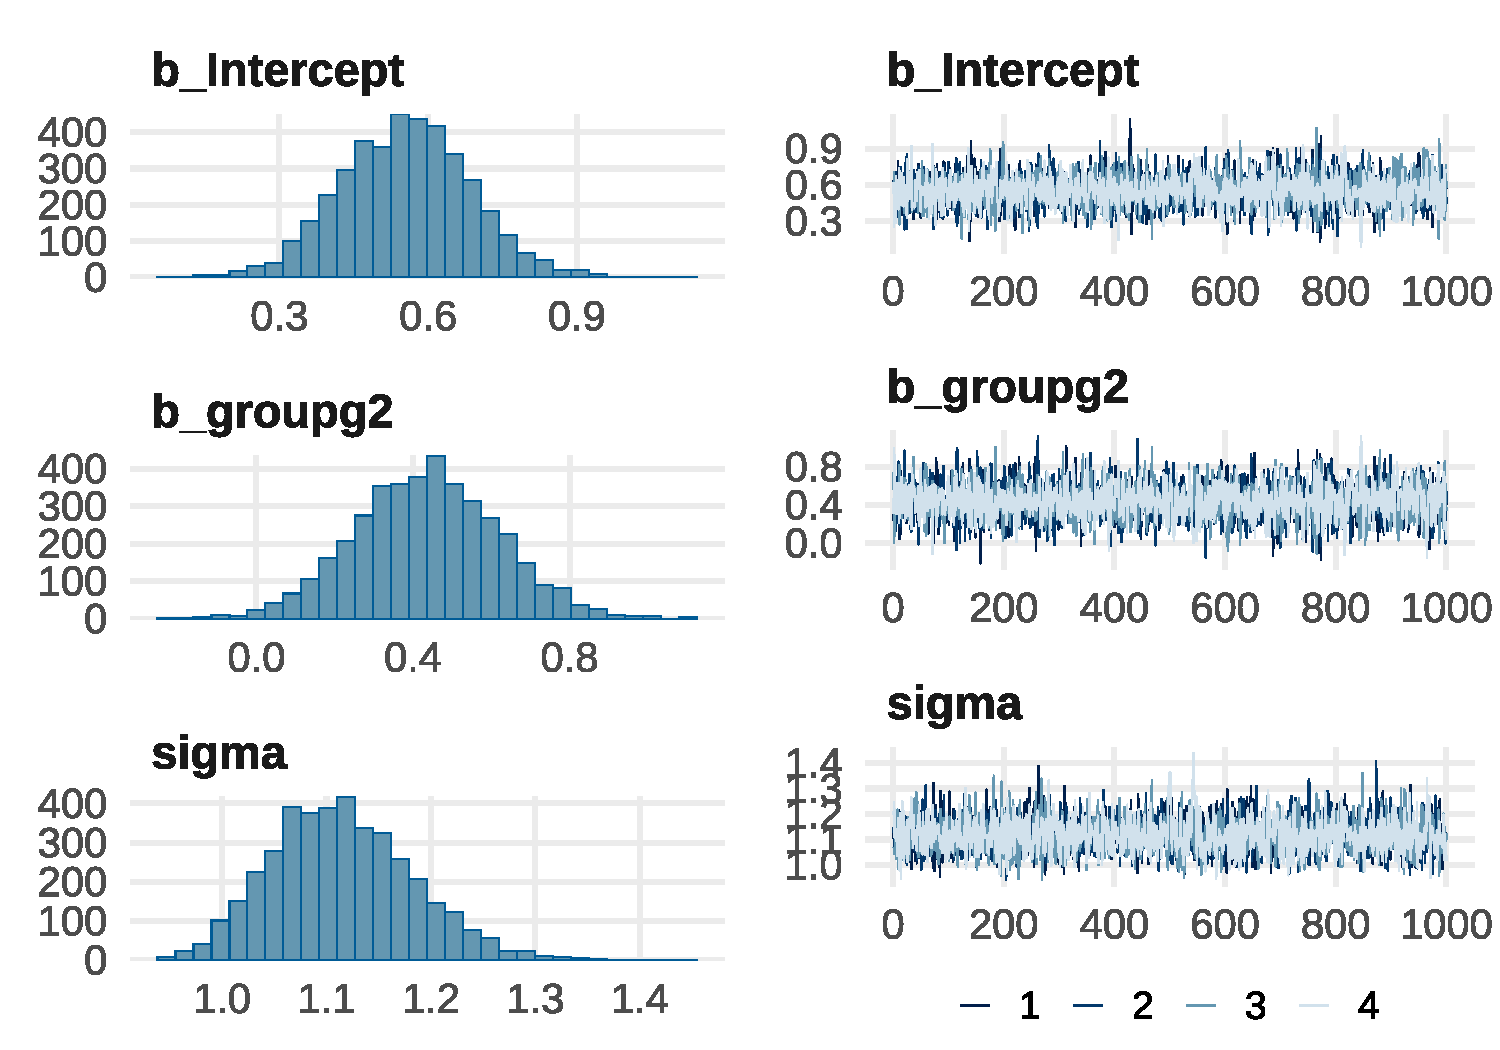
\includegraphics[keepaspectratio]{bayesian-glm_files/mediabag/bayesian-glm_files/figure-beamer/unnamed-chunk-32-1.pdf}}
\end{center}
\end{frame}

\begin{frame}{Model checking using simulations}
\phantomsection\label{model-checking-using-simulations}
We can check the model fit using simulations. In Bayesian terms this is
called Posterior Predictive Checks. For standard models we use only the
likelihood.

\begin{center}
\pandocbounded{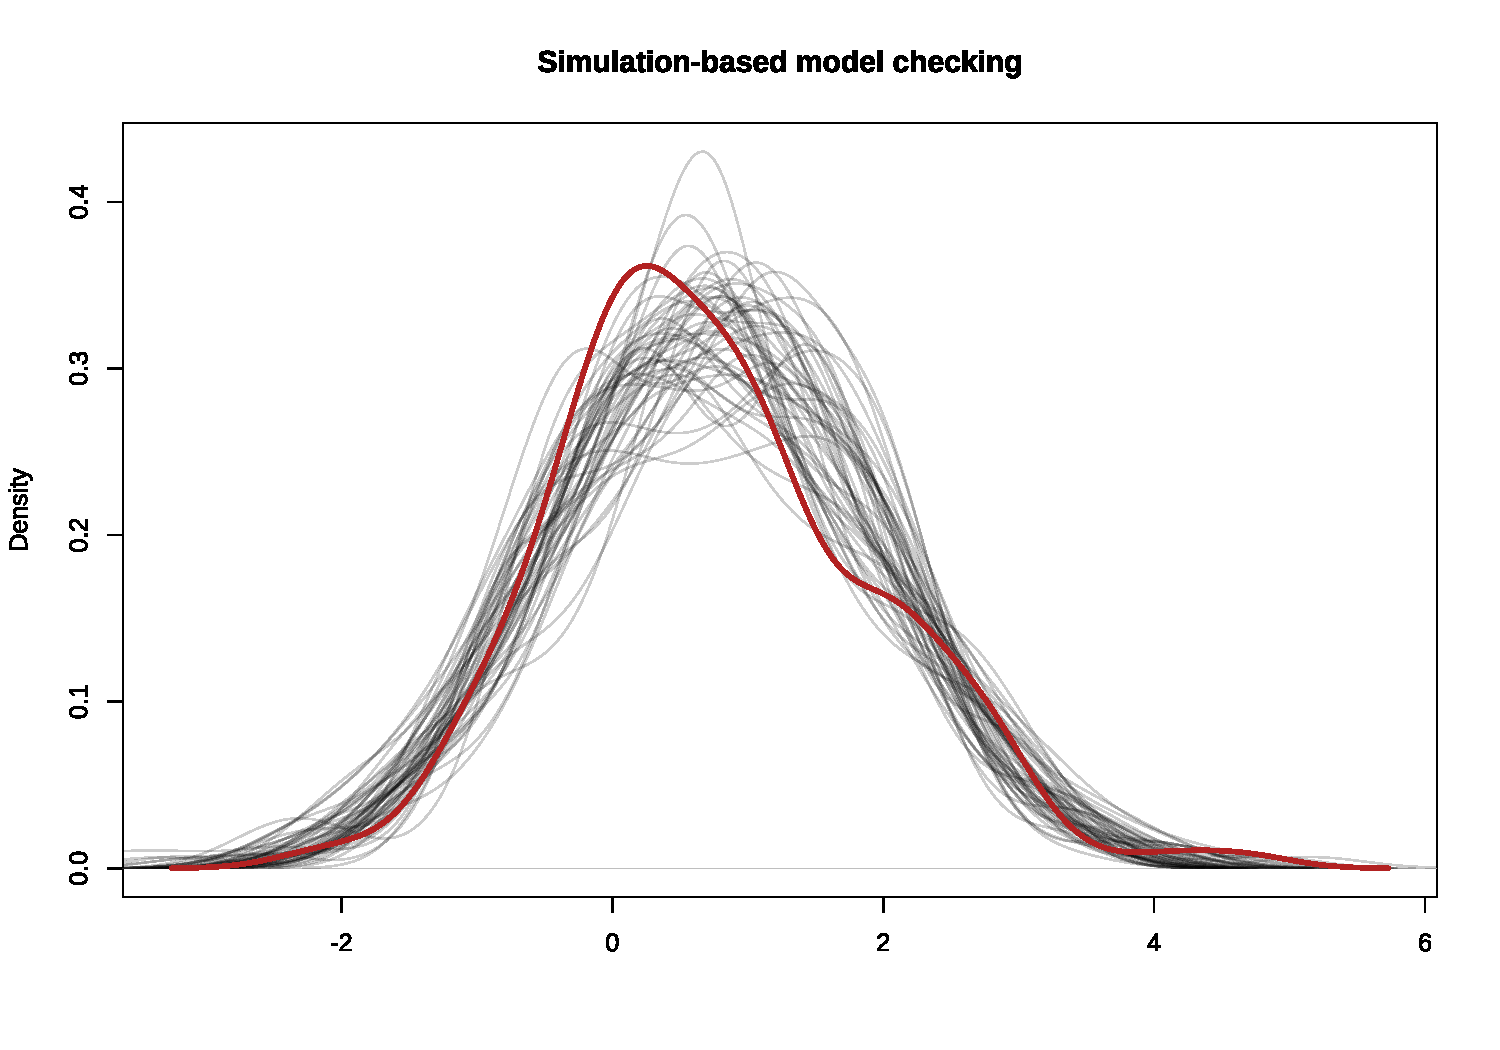
\includegraphics[keepaspectratio]{bayesian-glm_files/mediabag/bayesian-glm_files/figure-beamer/unnamed-chunk-33-1.pdf}}
\end{center}
\end{frame}

\begin{frame}[fragile]{Model checking using simulations}
\phantomsection\label{model-checking-using-simulations-1}
With the Bayesian models we can just use the \texttt{brms::pp\_check()}
function that compute the posterior predictive checks:

\begin{Shaded}
\begin{Highlighting}[]
\FunctionTok{pp\_check}\NormalTok{(fit\_group)}
\end{Highlighting}
\end{Shaded}

\begin{center}
\pandocbounded{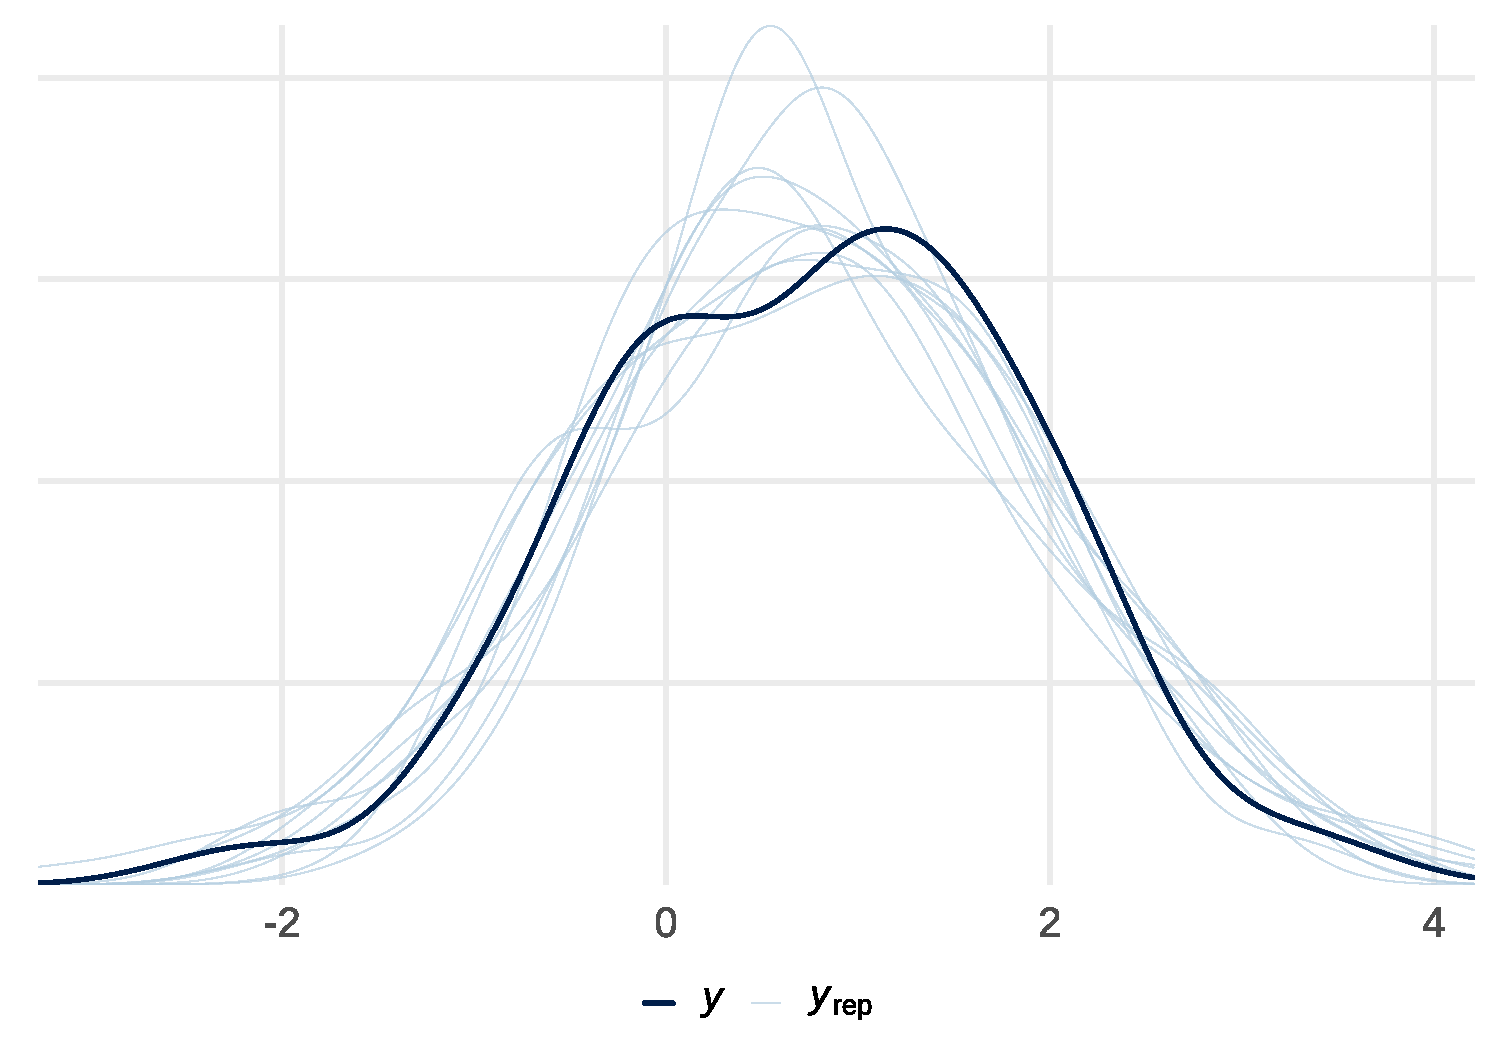
\includegraphics[keepaspectratio]{bayesian-glm_files/mediabag/bayesian-glm_files/figure-beamer/unnamed-chunk-34-1.pdf}}
\end{center}
\end{frame}

\begin{frame}[fragile]{Setting priors}
\phantomsection\label{setting-priors}
By default \texttt{brms} use some priors. You can see the actual used
priors using:

\begin{verbatim}
#>                   prior     class    coef group resp dpar nlpar lb ub
#>                  (flat)         b                                    
#>                  (flat)         b groupg2                            
#>  student_t(3, 0.9, 2.5) Intercept                                    
#>    student_t(3, 0, 2.5)     sigma                                0   
#>        source
#>       default
#>  (vectorized)
#>       default
#>       default
\end{verbatim}

You can also see the priors before fitting the model:

\begin{verbatim}
#>                   prior     class    coef group resp dpar nlpar lb ub
#>                  (flat)         b                                    
#>                  (flat)         b groupg2                            
#>  student_t(3, 0.6, 2.5) Intercept                                    
#>    student_t(3, 0, 2.5)     sigma                                0   
#>        source
#>       default
#>  (vectorized)
#>       default
#>       default
\end{verbatim}
\end{frame}

\section{Centering, re-scaling and contrasts
coding}\label{centering-re-scaling-and-contrasts-coding}

\begin{frame}{Centering, re-scaling and contrasts coding}
\phantomsection\label{centering-re-scaling-and-contrasts-coding-1}
When fitting a model is important to transform the predictors according
to the hypothesis that we have and the intepretation of parameters.

Centering (for numerical variables) and contrasts coding (for
categorical variables) are the two main strategies affecting the
intepretation of model parameters.

The crucial point is that also the prior distribution need to be adapted
when using different parametrizations of the same model.
\end{frame}

\begin{frame}{Rescaling}
\phantomsection\label{rescaling}
For example, let's assume to have the relationship between self-esteem
(from 0 to 20) and the graduation mark from 66 to 111 (110 cum laude):

\begin{center}
\pandocbounded{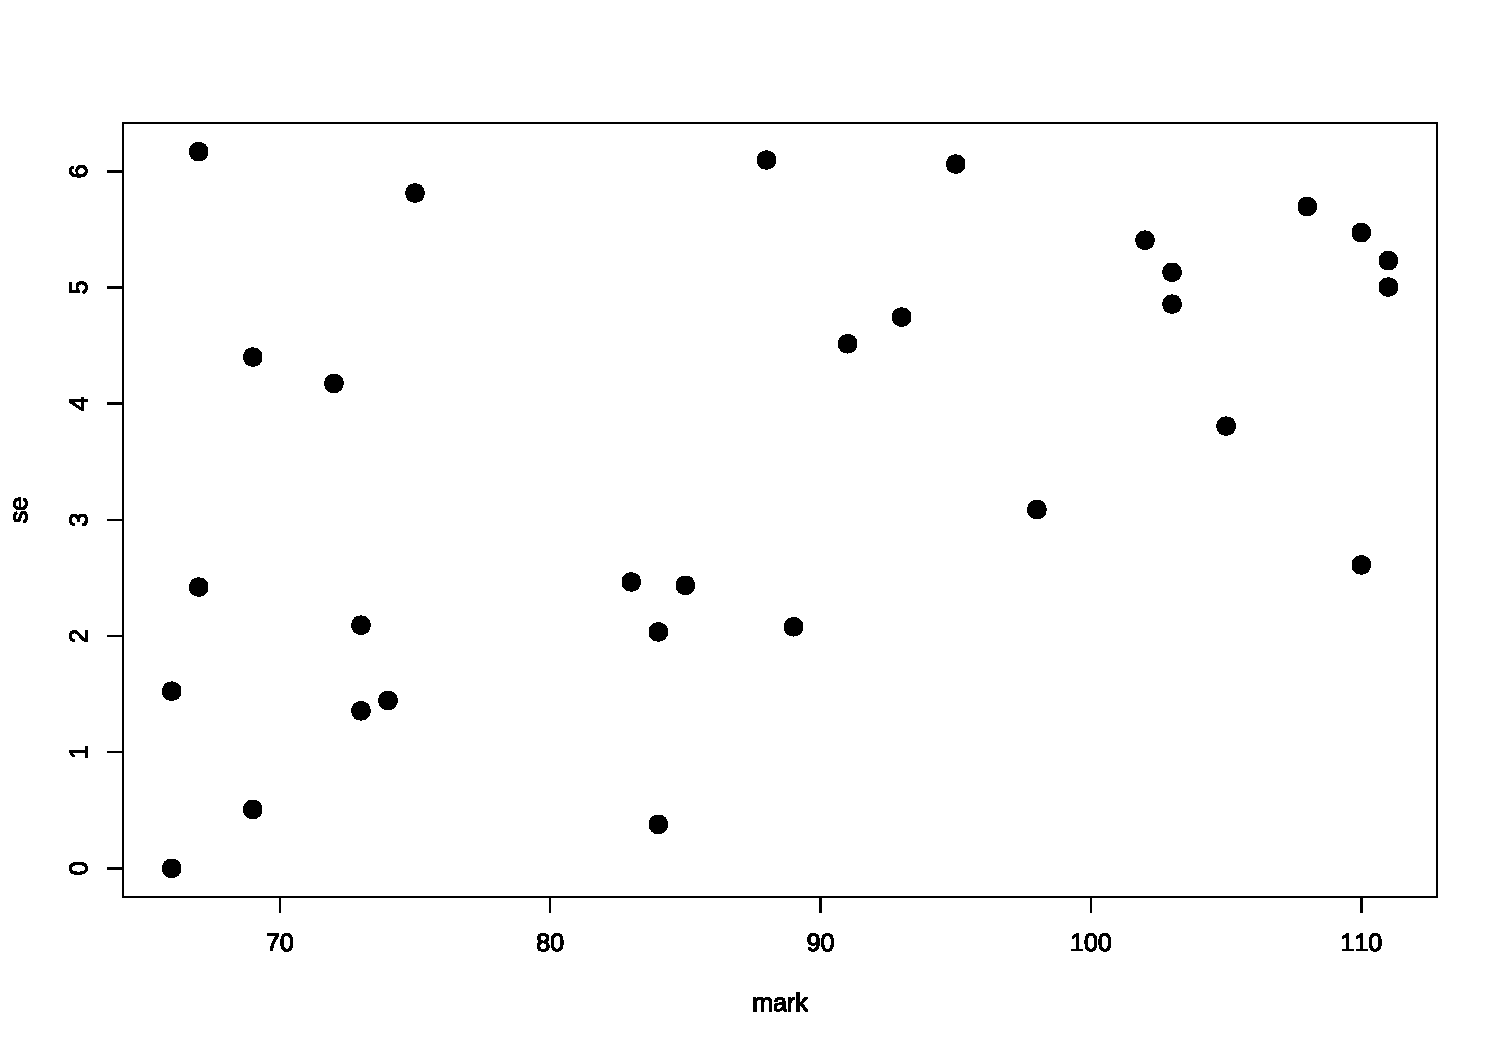
\includegraphics[keepaspectratio]{bayesian-glm_files/mediabag/bayesian-glm_files/figure-beamer/unnamed-chunk-38-1.pdf}}
\end{center}
\end{frame}

\begin{frame}[fragile]{Rescaling}
\phantomsection\label{rescaling-1}
Let's fit a simple regression:

\begin{verbatim}
#>  Family: gaussian 
#>   Links: mu = identity; sigma = identity 
#> Formula: se ~ mark 
#>    Data: dat_mark (Number of observations: 30) 
#>   Draws: 4 chains, each with iter = 2000; warmup = 1000; thin = 1;
#>          total post-warmup draws = 4000
#> 
#> Regression Coefficients:
#>           Estimate Est.Error l-95% CI u-95% CI Rhat Bulk_ESS Tail_ESS
#> Intercept    -7.96      2.10   -12.20    -3.85 1.00     3159     2822
#> mark          0.13      0.02     0.09     0.18 1.00     3186     2813
#> 
#> Further Distributional Parameters:
#>       Estimate Est.Error l-95% CI u-95% CI Rhat Bulk_ESS Tail_ESS
#> sigma     1.63      0.22     1.27     2.11 1.00     2741     2599
#> 
#> Draws were sampled using sampling(NUTS). For each parameter, Bulk_ESS
#> and Tail_ESS are effective sample size measures, and Rhat is the potential
#> scale reduction factor on split chains (at convergence, Rhat = 1).
\end{verbatim}
\end{frame}

\begin{frame}[fragile]{Rescaling, problems?}
\phantomsection\label{rescaling-problems}
We are using the default priors that are basically non-informative. What
about setting appropriate or more informative priors?

\begin{verbatim}
#>                   prior     class coef group resp dpar nlpar lb ub       source
#>                  (flat)         b                                       default
#>                  (flat)         b mark                             (vectorized)
#>  student_t(3, 3.9, 2.5) Intercept                                       default
#>    student_t(3, 0, 2.5)     sigma                             0         default
\end{verbatim}
\end{frame}

\begin{frame}[fragile]{Rescaling, problems?}
\phantomsection\label{rescaling-problems-1}
There are a couple of problems:

\begin{itemize}
\tightlist
\item
  \texttt{Intercept} is the expected self-esteem score for people with 0
  graduation mark (is that plausible?)
\item
  \texttt{mark} is the expected increase in self-esteem for a unit
  increase in the graduation mark. (is that intepretable?)
\end{itemize}

Assuming that we want to put priors, how do you choose the distribution
and the parameters?
\end{frame}

\begin{frame}[fragile]{Rescaling, problems?}
\phantomsection\label{rescaling-problems-2}
The first problem is that the \texttt{Intercept} is meaningless. Thus we
can, for example, mean-center the \texttt{mark} variable. The slope is
the same, we are only shifting the \texttt{x}. The intercept is
different.

\begin{center}
\pandocbounded{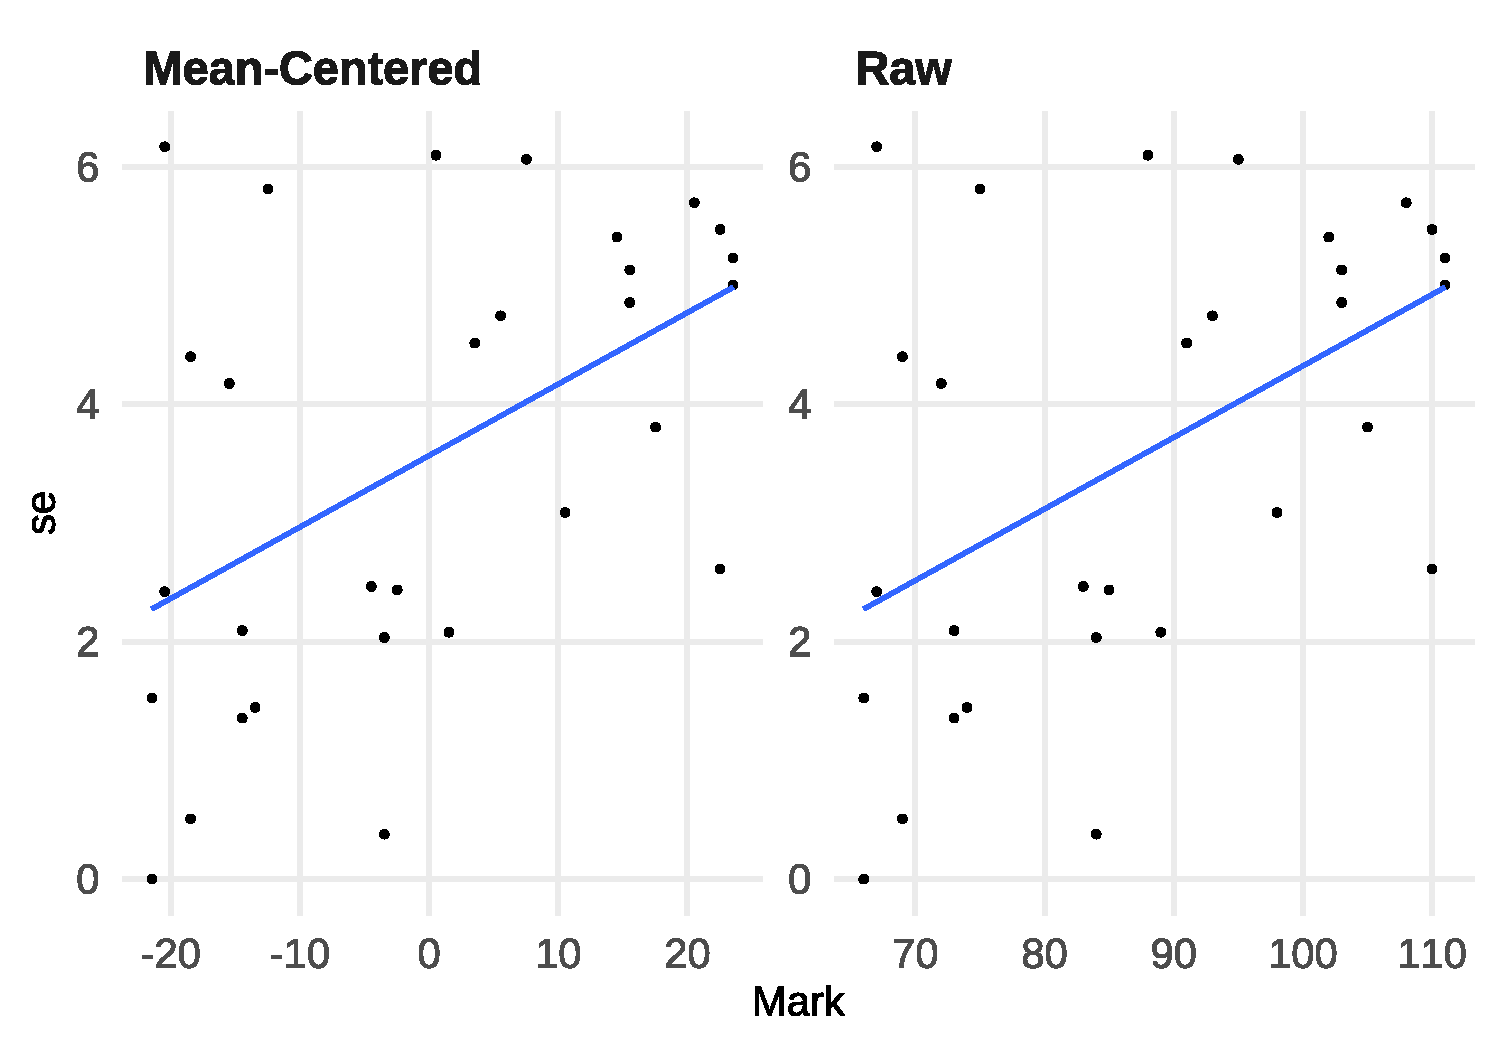
\includegraphics[keepaspectratio]{bayesian-glm_files/mediabag/bayesian-glm_files/figure-beamer/unnamed-chunk-41-1.pdf}}
\end{center}
\end{frame}

\begin{frame}[fragile]{Intercept prior}
\phantomsection\label{intercept-prior}
Now the intercept is the expected self esteem value when \texttt{mark}
is on average. Given that the values ranges from 0 to 20, we could put
less probability of extreme values (for average marks, around 88) we
could imagine also average value for self-esteem (around 10).

\begin{center}
\pandocbounded{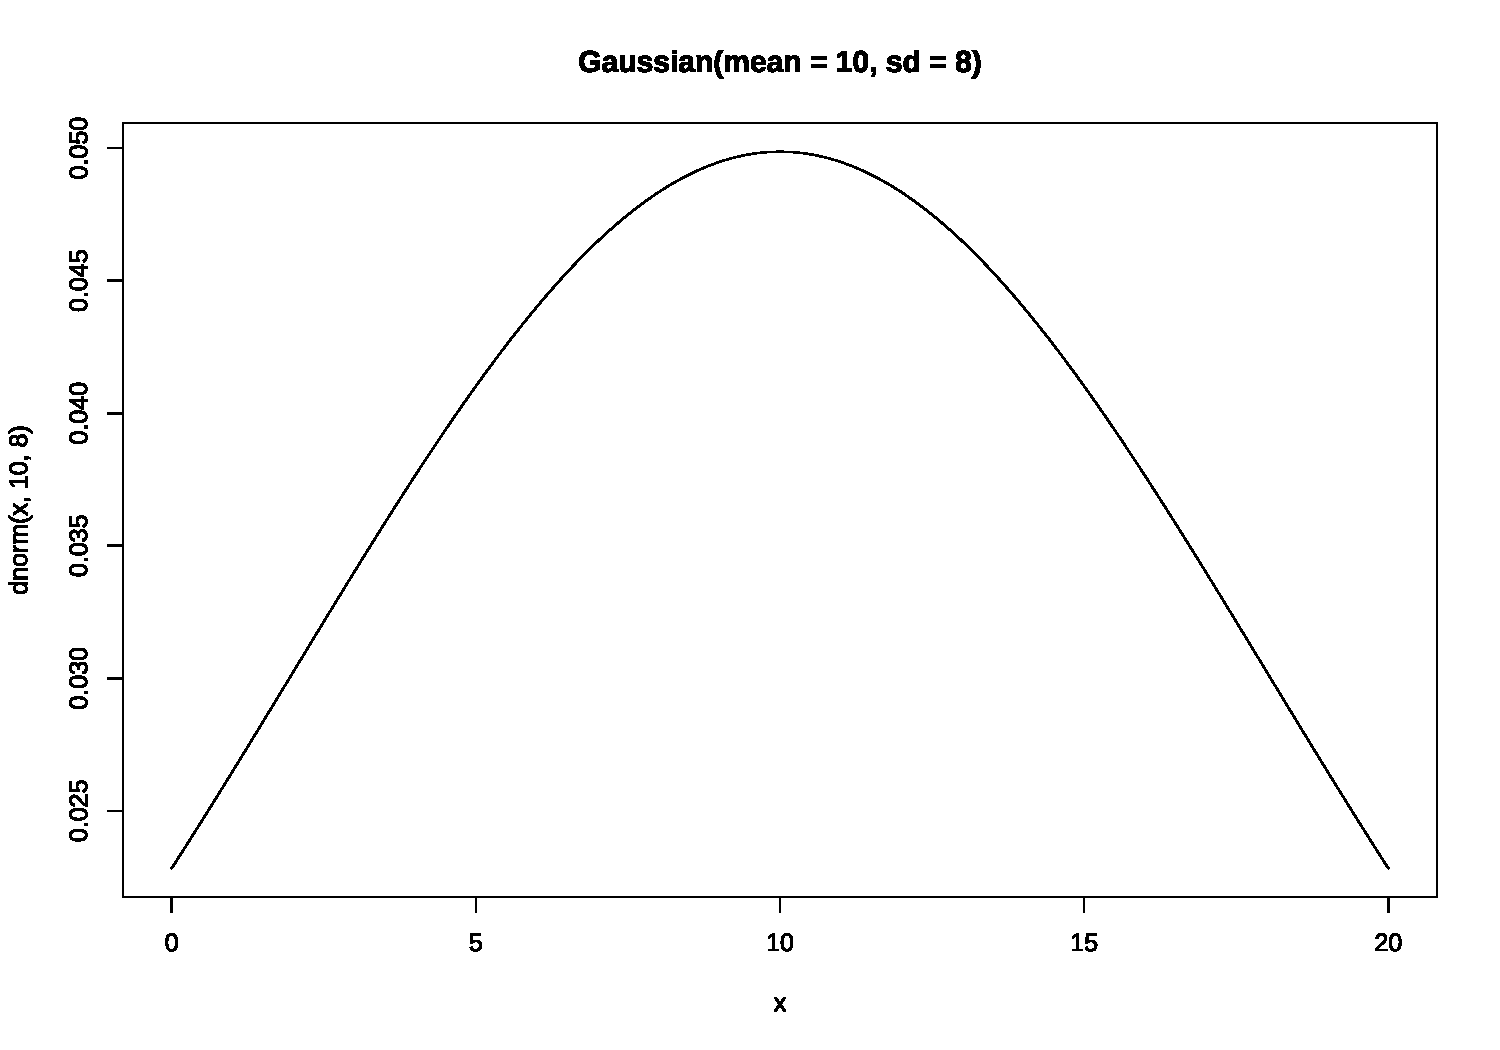
\includegraphics[keepaspectratio]{bayesian-glm_files/mediabag/bayesian-glm_files/figure-beamer/unnamed-chunk-42-1.pdf}}
\end{center}
\end{frame}

\begin{frame}[fragile]{Intercept prior, centering}
\phantomsection\label{intercept-prior-centering}
\begin{verbatim}
#> Intercept ~ normal(10, 8)
\end{verbatim}
\end{frame}

\begin{frame}[fragile]{Slope prior, rescaling}
\phantomsection\label{slope-prior-rescaling}
Then for the slope, probably there is too much granularity in the
\texttt{mark} variable. 1 point increase is very tiny. To improve the
model interpretation we can rescale the variable giving more weight to
the unit increase.

\begin{center}
\pandocbounded{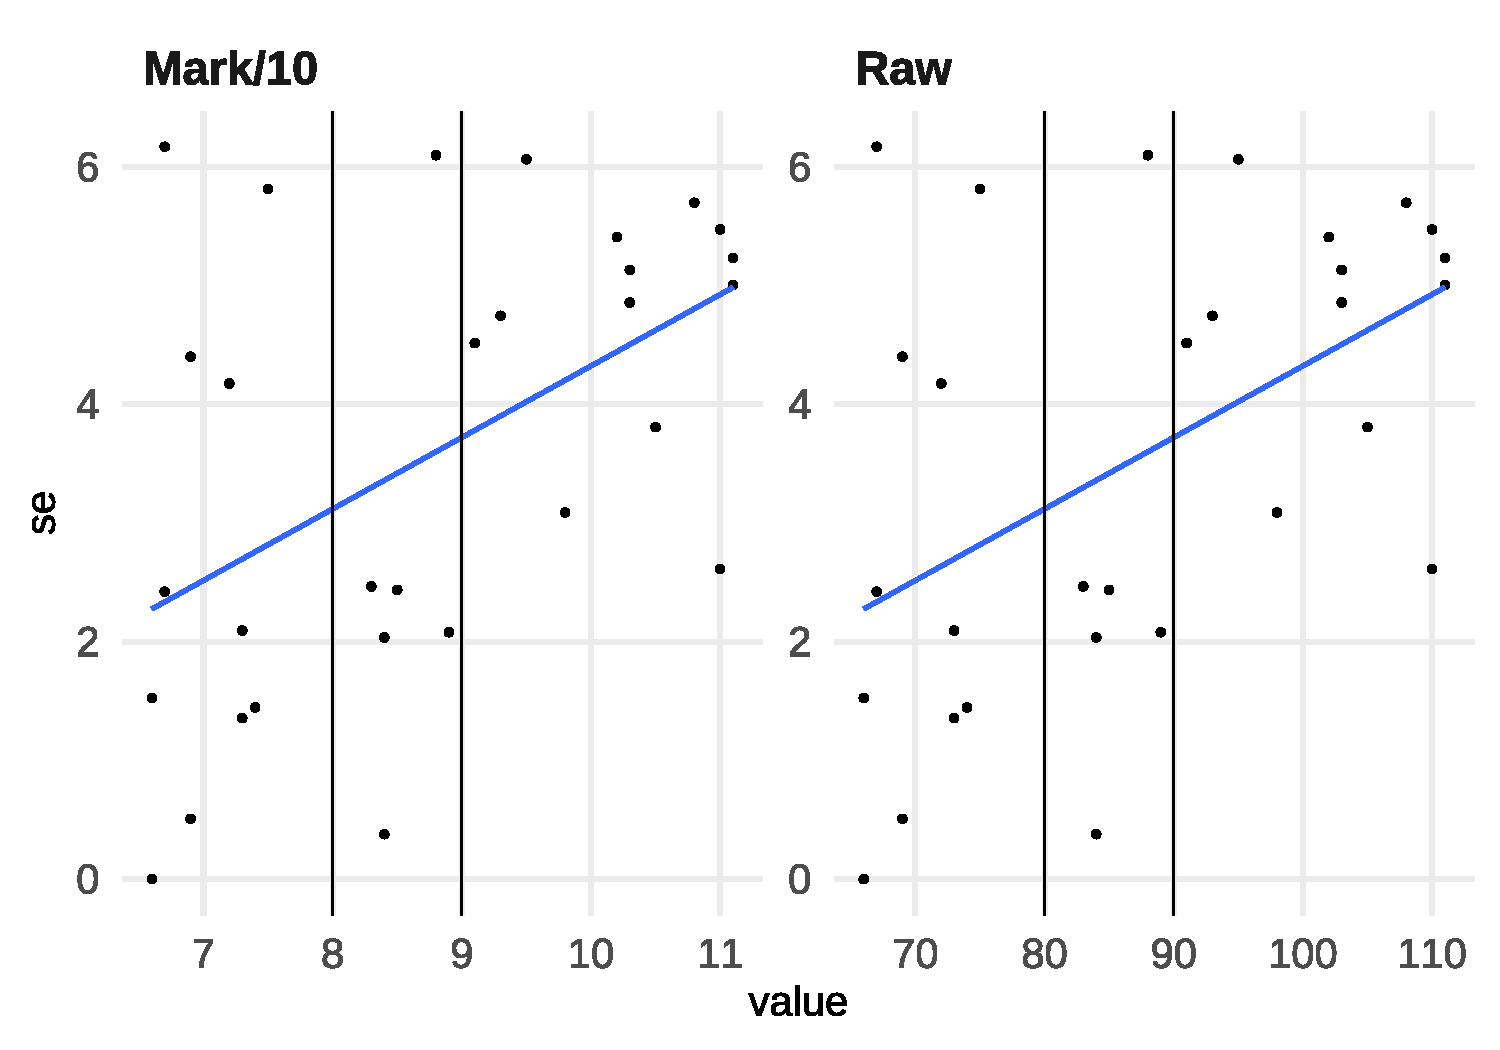
\includegraphics[keepaspectratio]{bayesian-glm_files/mediabag/bayesian-glm_files/figure-beamer/unnamed-chunk-44-1.pdf}}
\end{center}
\end{frame}

\begin{frame}{Slope prior, rescaling}
\phantomsection\label{slope-prior-rescaling-1}
Now we have a more practical idea of size of the slope. We can use a
very vague but not flat prior (the default) considering that 0 means no
effect. Remember that now the slope is the increase in self-esteem for
incrase of 10 points in the mark.

\begin{center}
\pandocbounded{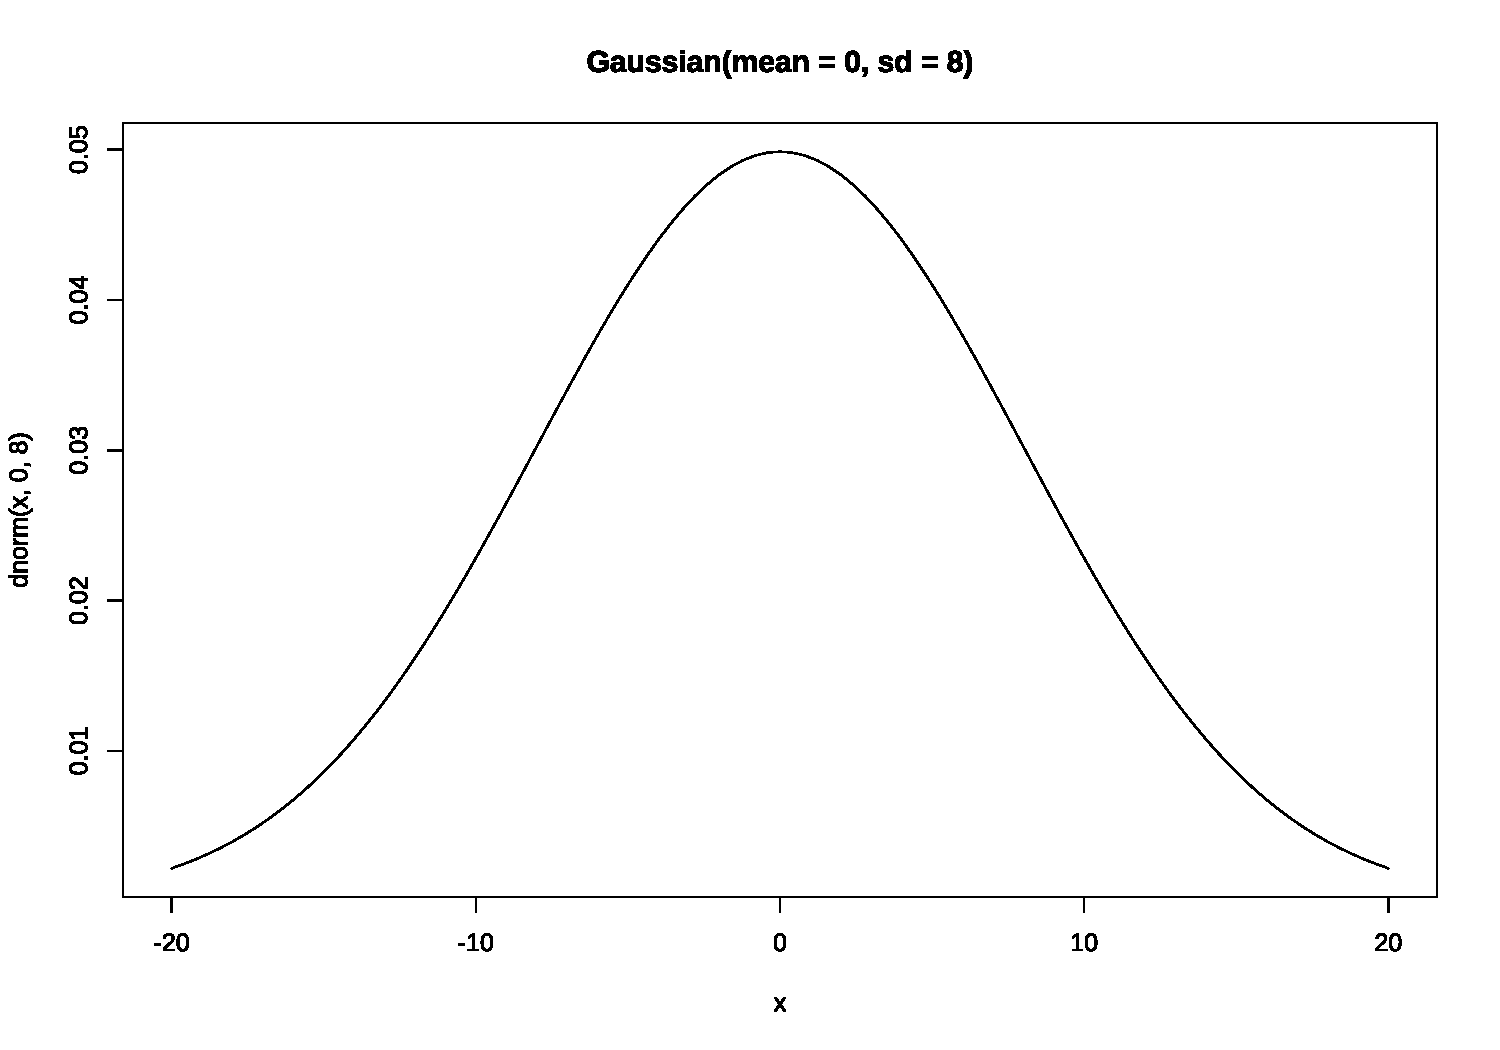
\includegraphics[keepaspectratio]{bayesian-glm_files/mediabag/bayesian-glm_files/figure-beamer/unnamed-chunk-45-1.pdf}}
\end{center}
\end{frame}

\begin{frame}{Slope prior, rescaling}
\phantomsection\label{slope-prior-rescaling-2}
The previus prior is very uninformative but is simply excluding
impossible values. A slope of 10 means that increasing by 10 points
would produce an increase that ranges the entire available scale.
\end{frame}

\begin{frame}[fragile]{Refitting the model\footnote<.->[frame]{For the
  residual standard deviation, \texttt{brms} is already doing a good job
  with default priors, mainly escluding negative values.}}
\phantomsection\label{refitting-the-model}
We can now refit the model using our priors and rescaling/centering

\begin{verbatim}
#>  Family: gaussian 
#>   Links: mu = identity; sigma = identity 
#> Formula: se ~ mark10c 
#>    Data: dat_mark (Number of observations: 30) 
#>   Draws: 4 chains, each with iter = 2000; warmup = 1000; thin = 1;
#>          total post-warmup draws = 4000
#> 
#> Regression Coefficients:
#>           Estimate Est.Error l-95% CI u-95% CI Rhat Bulk_ESS Tail_ESS
#> Intercept     3.58      0.32     2.95     4.23 1.00     3172     2437
#> mark10c       0.60      0.21     0.18     0.99 1.00     3775     2708
#> 
#> Further Distributional Parameters:
#>       Estimate Est.Error l-95% CI u-95% CI Rhat Bulk_ESS Tail_ESS
#> sigma     1.75      0.24     1.35     2.31 1.00     3378     2792
#> 
#> Draws were sampled using sampling(NUTS). For each parameter, Bulk_ESS
#> and Tail_ESS are effective sample size measures, and Rhat is the potential
#> scale reduction factor on split chains (at convergence, Rhat = 1).
\end{verbatim}
\end{frame}

\begin{frame}[fragile]{Contrasts coding}
\phantomsection\label{contrasts-coding}
Contrasts coding is a vast and difficult topic. The basic idea is that
when you have categorical predictors, with or without interactions, the
way you set the contrasts will impact the intepretation of model
parameters (and the priors).

By default in R, categorical variables are coded using the so-called
\textbf{dummy coding} or \textbf{treatment coding}.

\begin{Shaded}
\begin{Highlighting}[]
\NormalTok{x }\OtherTok{\textless{}{-}} \FunctionTok{factor}\NormalTok{(}\FunctionTok{rep}\NormalTok{(}\FunctionTok{c}\NormalTok{(}\StringTok{"a"}\NormalTok{, }\StringTok{"b"}\NormalTok{, }\StringTok{"c"}\NormalTok{), }\AttributeTok{each =} \DecValTok{5}\NormalTok{))}
\NormalTok{x}
\end{Highlighting}
\end{Shaded}

\begin{verbatim}
#>  [1] a a a a a b b b b b c c c c c
#> Levels: a b c
\end{verbatim}
\end{frame}

\begin{frame}[fragile]{Contrasts coding}
\phantomsection\label{contrasts-coding-1}
\begin{Shaded}
\begin{Highlighting}[]
\FunctionTok{contrasts}\NormalTok{(x)}
\end{Highlighting}
\end{Shaded}

\begin{verbatim}
#>   b c
#> a 0 0
#> b 1 0
#> c 0 1
\end{verbatim}

\begin{Shaded}
\begin{Highlighting}[]
\FunctionTok{model.matrix}\NormalTok{(}\SpecialCharTok{\textasciitilde{}}\NormalTok{x)}
\end{Highlighting}
\end{Shaded}

\begin{verbatim}
#>    (Intercept) xb xc
#> 1            1  0  0
#> 2            1  0  0
#> 3            1  0  0
#> 4            1  0  0
#> 5            1  0  0
#> 6            1  1  0
#> 7            1  1  0
#> 8            1  1  0
#> 9            1  1  0
#> 10           1  1  0
#> 11           1  0  1
#> 12           1  0  1
#> 13           1  0  1
#> 14           1  0  1
#> 15           1  0  1
#> attr(,"assign")
#> [1] 0 1 1
#> attr(,"contrasts")
#> attr(,"contrasts")$x
#> [1] "contr.treatment"
\end{verbatim}
\end{frame}

\begin{frame}[fragile]{Contrasts coding}
\phantomsection\label{contrasts-coding-2}
With a factor with \(p\) levels, we need \(p - 1\) variables
representing contrasts. \textbf{dummy-coding} means that there will be a
reference level (usually the first level) and \(p - 1\) contrasts
comparing the other levels with the first level (baseline).

An example with the \texttt{iris} dataset:

\begin{Shaded}
\begin{Highlighting}[]
\FunctionTok{levels}\NormalTok{(iris}\SpecialCharTok{$}\NormalTok{Species)}
\CommentTok{\#\textgreater{} [1] "setosa"     "versicolor" "virginica"}
\NormalTok{fit\_dummy }\OtherTok{\textless{}{-}} \FunctionTok{lm}\NormalTok{(Sepal.Length }\SpecialCharTok{\textasciitilde{}}\NormalTok{ Species, }\AttributeTok{data =}\NormalTok{ iris)}
\FunctionTok{summary}\NormalTok{(fit\_dummy)}
\CommentTok{\#\textgreater{} }
\CommentTok{\#\textgreater{} Call:}
\CommentTok{\#\textgreater{} lm(formula = Sepal.Length \textasciitilde{} Species, data = iris)}
\CommentTok{\#\textgreater{} }
\CommentTok{\#\textgreater{} Residuals:}
\CommentTok{\#\textgreater{}     Min      1Q  Median      3Q     Max }
\CommentTok{\#\textgreater{} {-}1.6880 {-}0.3285 {-}0.0060  0.3120  1.3120 }
\CommentTok{\#\textgreater{} }
\CommentTok{\#\textgreater{} Coefficients:}
\CommentTok{\#\textgreater{}                   Estimate Std. Error t value Pr(\textgreater{}|t|)    }
\CommentTok{\#\textgreater{} (Intercept)         5.0060     0.0728  68.762  \textless{} 2e{-}16 ***}
\CommentTok{\#\textgreater{} Speciesversicolor   0.9300     0.1030   9.033 8.77e{-}16 ***}
\CommentTok{\#\textgreater{} Speciesvirginica    1.5820     0.1030  15.366  \textless{} 2e{-}16 ***}
\CommentTok{\#\textgreater{} {-}{-}{-}}
\CommentTok{\#\textgreater{} Signif. codes:  0 \textquotesingle{}***\textquotesingle{} 0.001 \textquotesingle{}**\textquotesingle{} 0.01 \textquotesingle{}*\textquotesingle{} 0.05 \textquotesingle{}.\textquotesingle{} 0.1 \textquotesingle{} \textquotesingle{} 1}
\CommentTok{\#\textgreater{} }
\CommentTok{\#\textgreater{} Residual standard error: 0.5148 on 147 degrees of freedom}
\CommentTok{\#\textgreater{} Multiple R{-}squared:  0.6187, Adjusted R{-}squared:  0.6135 }
\CommentTok{\#\textgreater{} F{-}statistic: 119.3 on 2 and 147 DF,  p{-}value: \textless{} 2.2e{-}16}
\end{Highlighting}
\end{Shaded}
\end{frame}

\begin{frame}[fragile]{Contrasts coding}
\phantomsection\label{contrasts-coding-3}
\begin{Shaded}
\begin{Highlighting}[]
\NormalTok{vv }\OtherTok{\textless{}{-}} \FunctionTok{split}\NormalTok{(iris}\SpecialCharTok{$}\NormalTok{Sepal.Length, iris}\SpecialCharTok{$}\NormalTok{Species)}
\FunctionTok{mean}\NormalTok{(vv}\SpecialCharTok{$}\NormalTok{setosa)}
\end{Highlighting}
\end{Shaded}

\begin{verbatim}
#> [1] 5.006
\end{verbatim}

\begin{Shaded}
\begin{Highlighting}[]
\FunctionTok{mean}\NormalTok{(vv}\SpecialCharTok{$}\NormalTok{versicolor) }\SpecialCharTok{{-}} \FunctionTok{mean}\NormalTok{(vv}\SpecialCharTok{$}\NormalTok{setosa)}
\end{Highlighting}
\end{Shaded}

\begin{verbatim}
#> [1] 0.93
\end{verbatim}

\begin{Shaded}
\begin{Highlighting}[]
\FunctionTok{mean}\NormalTok{(vv}\SpecialCharTok{$}\NormalTok{virginica) }\SpecialCharTok{{-}} \FunctionTok{mean}\NormalTok{(vv}\SpecialCharTok{$}\NormalTok{setosa)}
\end{Highlighting}
\end{Shaded}

\begin{verbatim}
#> [1] 1.582
\end{verbatim}
\end{frame}

\begin{frame}[fragile]{Contrasts coding}
\phantomsection\label{contrasts-coding-4}
Another coding scheme could be the so called \textbf{Successive
Differences Contrast Coding}. The idea is to compare level 2 with level
1, level 3 with level 2 and so on.

\begin{Shaded}
\begin{Highlighting}[]
\NormalTok{iris}\SpecialCharTok{$}\NormalTok{Species\_sdif }\OtherTok{\textless{}{-}}\NormalTok{ iris}\SpecialCharTok{$}\NormalTok{Species}
\FunctionTok{contrasts}\NormalTok{(iris}\SpecialCharTok{$}\NormalTok{Species\_sdif) }\OtherTok{\textless{}{-}}\NormalTok{ MASS}\SpecialCharTok{::}\FunctionTok{contr.sdif}\NormalTok{(}\DecValTok{3}\NormalTok{)}
\FunctionTok{contrasts}\NormalTok{(iris}\SpecialCharTok{$}\NormalTok{Species\_sdif)}
\end{Highlighting}
\end{Shaded}

\begin{verbatim}
#>                   2-1        3-2
#> setosa     -0.6666667 -0.3333333
#> versicolor  0.3333333 -0.3333333
#> virginica   0.3333333  0.6666667
\end{verbatim}
\end{frame}

\begin{frame}[fragile]{Contrasts coding}
\phantomsection\label{contrasts-coding-5}
\begin{Shaded}
\begin{Highlighting}[]
\NormalTok{fit\_sdif }\OtherTok{\textless{}{-}} \FunctionTok{lm}\NormalTok{(Sepal.Length }\SpecialCharTok{\textasciitilde{}}\NormalTok{ Species\_sdif, }\AttributeTok{data =}\NormalTok{ iris)}
\FunctionTok{summary}\NormalTok{(fit\_sdif)}
\end{Highlighting}
\end{Shaded}

\begin{verbatim}
#> 
#> Call:
#> lm(formula = Sepal.Length ~ Species_sdif, data = iris)
#> 
#> Residuals:
#>     Min      1Q  Median      3Q     Max 
#> -1.6880 -0.3285 -0.0060  0.3120  1.3120 
#> 
#> Coefficients:
#>                 Estimate Std. Error t value Pr(>|t|)    
#> (Intercept)      5.84333    0.04203 139.020  < 2e-16 ***
#> Species_sdif2-1  0.93000    0.10296   9.033 8.77e-16 ***
#> Species_sdif3-2  0.65200    0.10296   6.333 2.77e-09 ***
#> ---
#> Signif. codes:  0 '***' 0.001 '**' 0.01 '*' 0.05 '.' 0.1 ' ' 1
#> 
#> Residual standard error: 0.5148 on 147 degrees of freedom
#> Multiple R-squared:  0.6187, Adjusted R-squared:  0.6135 
#> F-statistic: 119.3 on 2 and 147 DF,  p-value: < 2.2e-16
\end{verbatim}
\end{frame}

\begin{frame}{More on contrasts coding}
\phantomsection\label{more-on-contrasts-coding}
There are few very useful papers about contrasts coding:

\begin{itemize}
\tightlist
\item
  Schad et al. (\citeproc{ref-Schad2020-ht}{2020}): comprehensive and
  (difficult) paper about contrasts coding
\item
  Granziol et al. (\citeproc{ref-Granziol2025-sy}{2025}): amazing work
  by our colleagues in Padova
\end{itemize}
\end{frame}

\section{Hypothesis testing and effect
size}\label{hypothesis-testing-and-effect-size}

\begin{frame}{Hypothesis testing}
\phantomsection\label{hypothesis-testing}
The easiest way to test an hypothesis similarly to the frequentist
framework is by checking if the null value of a certain test is contaned
or not in the Credible Interval or the Highest Posterior Density
Interval.

In the frequentist framework, the p value lower than \(\alpha\)
corresponds to a confidence interval to \(1 - \alpha\) level that does
not contains the null value (e.g., 0).
\end{frame}

\begin{frame}[fragile]{\texttt{brms::hypothesis()}}
\phantomsection\label{brmshypothesis}
The \texttt{brms::hypothesis()} function is a very nice way to test
hypotheses into a bayesian framework.

\begin{center}
\pandocbounded{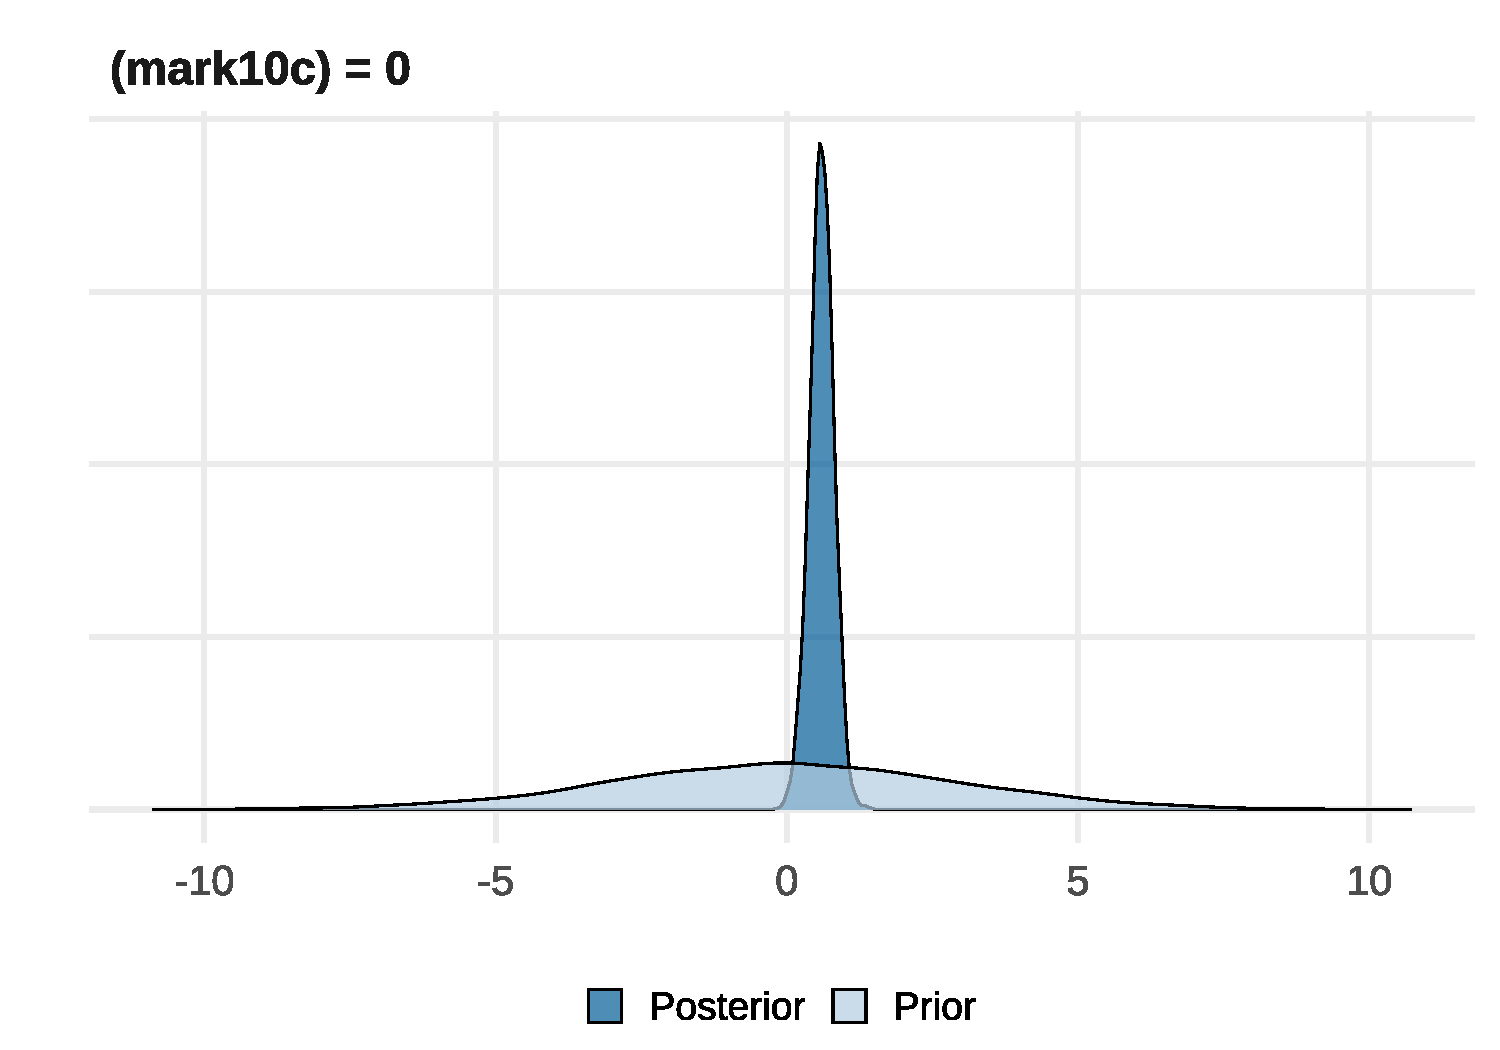
\includegraphics[keepaspectratio]{bayesian-glm_files/mediabag/bayesian-glm_files/figure-beamer/unnamed-chunk-54-1.pdf}}
\end{center}
\end{frame}

\begin{frame}{Bayesian \(R^2\) (\citeproc{ref-Gelman2019-hp}{Gelman et
al. 2019})}
\phantomsection\label{bayesian-r2-gelman2019-hp}
Gelman et al. (\citeproc{ref-Gelman2019-hp}{2019}) explained a
generalization of the common \(R^2\) to be applied for Bayesian
Generalized Linear Models.

\[
\text{Bayesian } R^2_s = 
\frac{
\mathrm{Var}_{n=1}^{N}\left( y_n^{\text{pred}, s} \right)
}{
\mathrm{Var}_{n=1}^{N}\left( y_n^{\text{pred}, s} \right) + \mathrm{Var}_{\text{res}}^s
}
\]

There are few important points:

\begin{itemize}
\tightlist
\item
  This works for any GLM (unlike the usual \(R^2\))
\item
  Different models on the same dataset cannot be compared
  https://avehtari.github.io/bayes\_R2/bayes\_R2.html
\end{itemize}
\end{frame}

\begin{frame}{Extracting posteriors}
\phantomsection\label{extracting-posteriors}
https://www.andrewheiss.com/blog/2022/09/26/guide-visualizing-types-posteriors/
https://www.andrewheiss.com/blog/2022/09/26/guide-visualizing-types-posteriors/\#complete-cheat-sheet
\end{frame}

\begin{frame}{Bayes Factor}
\phantomsection\label{bayes-factor}
As an example we can start with the classical coin-flip experiment. We
need to guess if a coin is fair or not. Firstly let's formalize our
prior beliefs in probabilistic terms:

\begin{center}
\pandocbounded{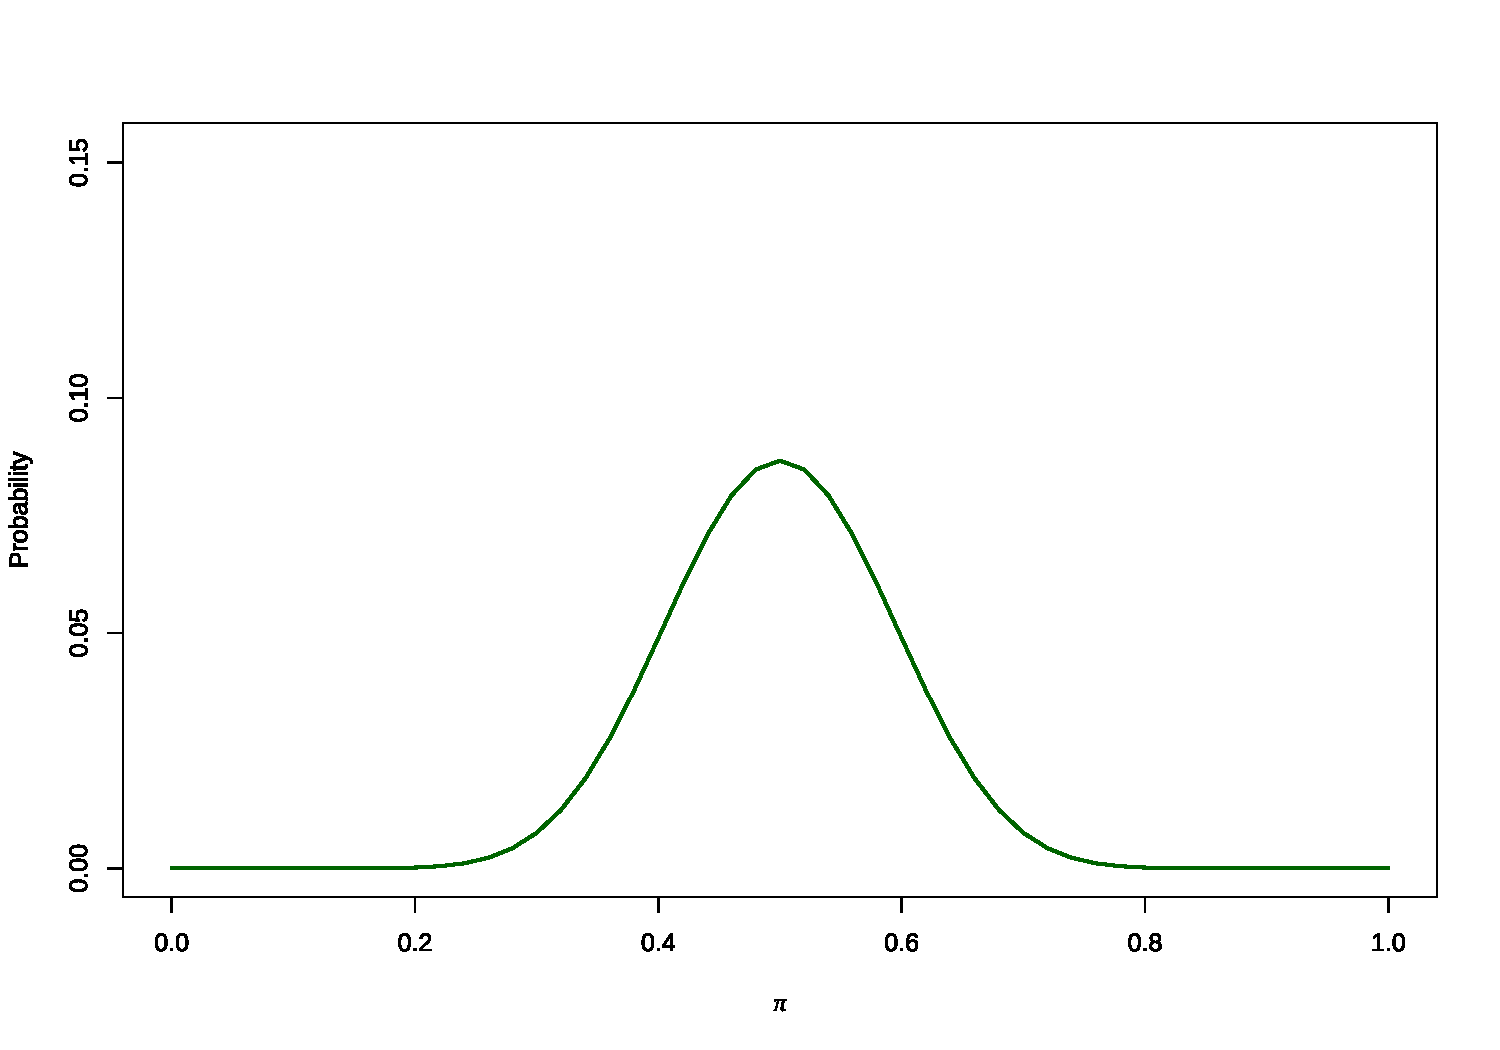
\includegraphics[keepaspectratio]{bayesian-glm_files/mediabag/bayesian-glm_files/figure-beamer/unnamed-chunk-55-1.pdf}}
\end{center}
\end{frame}

\begin{frame}{Bayes Factor}
\phantomsection\label{bayes-factor-1}
Now we collect data and we observe \(x = 40\) tails out of \(k = 50\)
trials thus \(\hat{\pi} = 0.8\) and compute the \emph{likelihood}:

\begin{center}
\pandocbounded{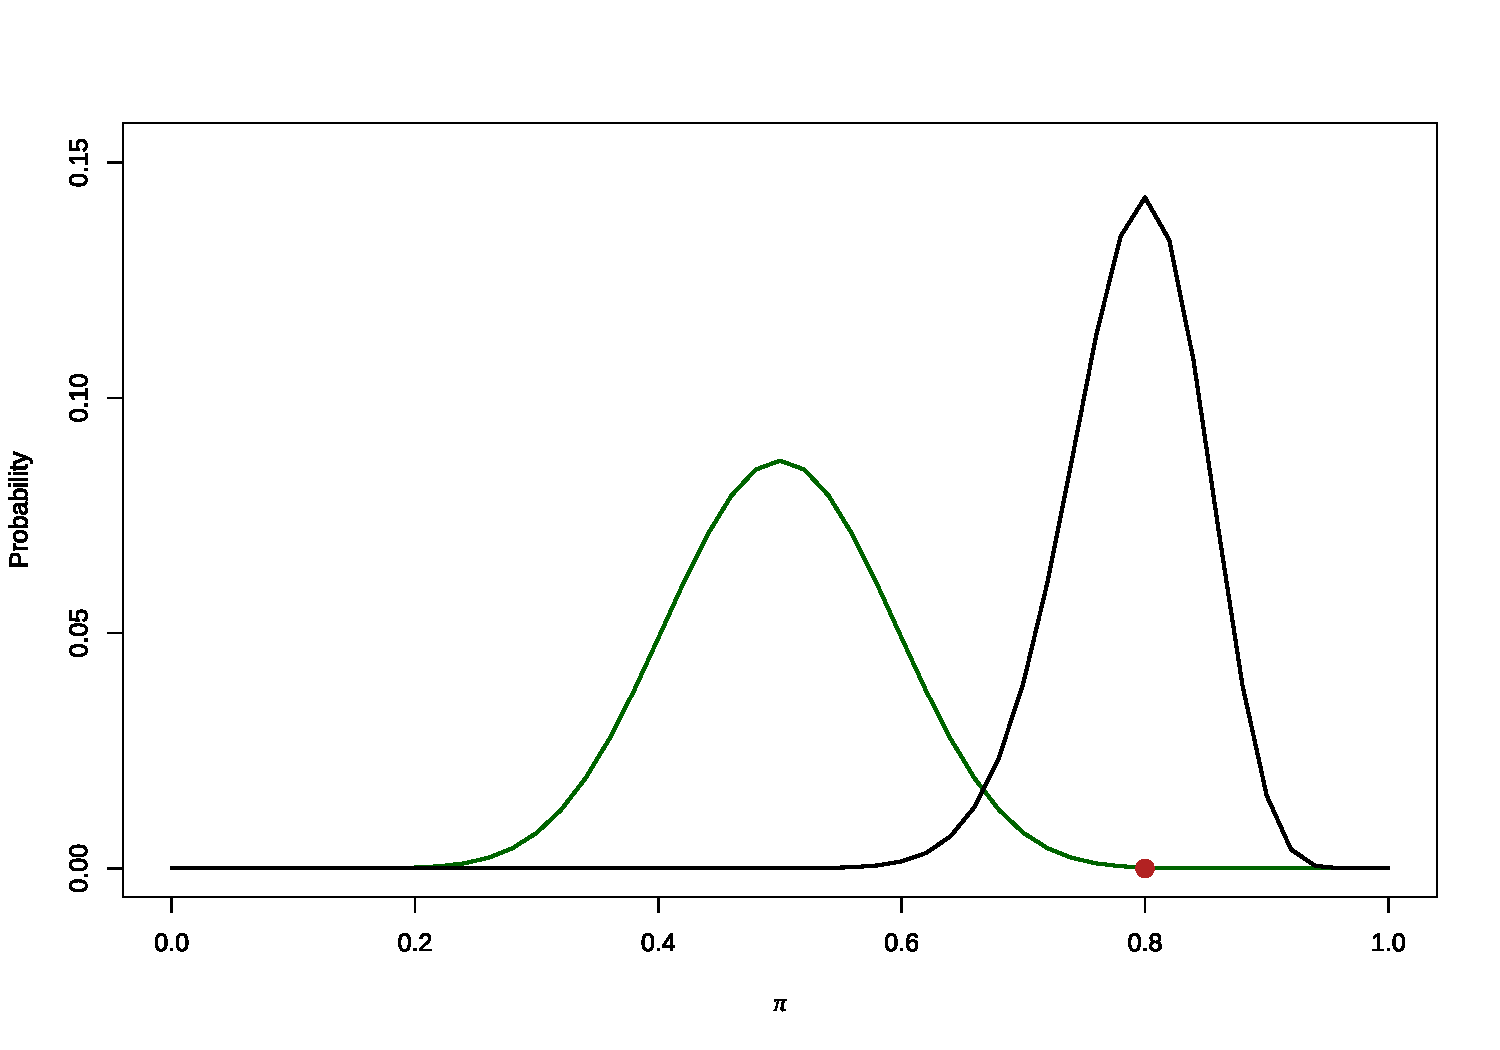
\includegraphics[keepaspectratio]{bayesian-glm_files/mediabag/bayesian-glm_files/figure-beamer/unnamed-chunk-56-1.pdf}}
\end{center}
\end{frame}

\begin{frame}{Bayes Factor}
\phantomsection\label{bayes-factor-2}
Finally we combine, using the Bayes rule, \textbf{prior} and
\textbf{likelihood} to obtain the \textbf{posterior} distribution:

\begin{center}
\pandocbounded{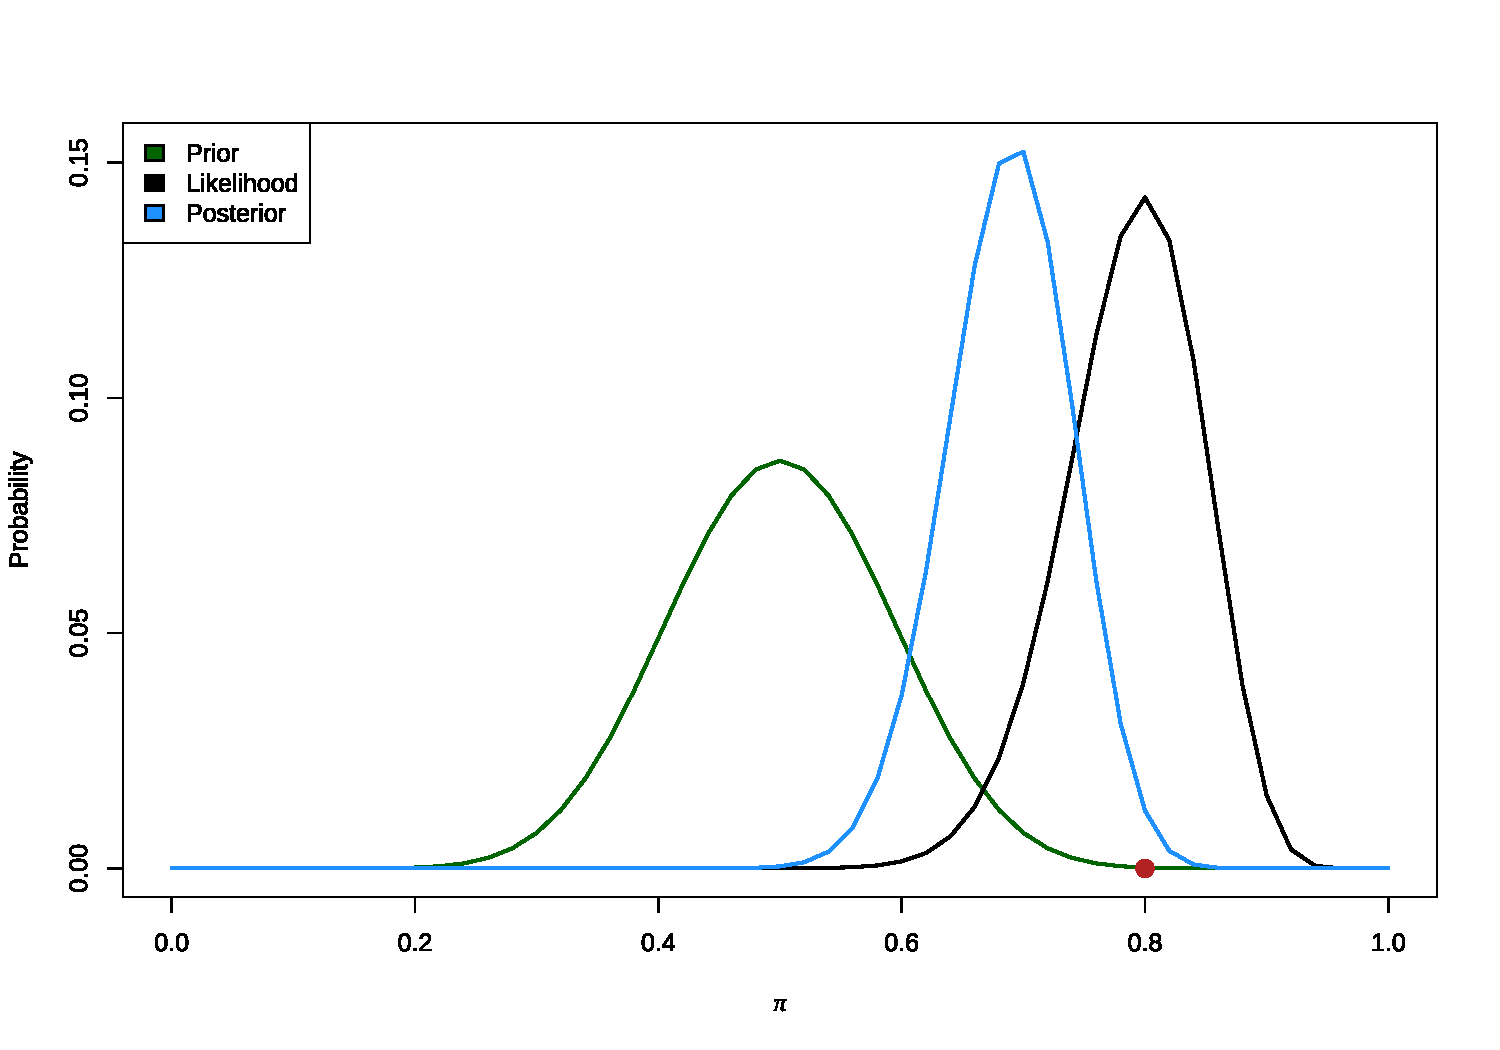
\includegraphics[keepaspectratio]{bayesian-glm_files/mediabag/bayesian-glm_files/figure-beamer/unnamed-chunk-57-1.pdf}}
\end{center}
\end{frame}

\begin{frame}{Bayes Factor}
\phantomsection\label{bayes-factor-3}
The \textbf{Bayes Factor} (BF) --- also called the \textbf{likelihood
ratio}, for obvious reasons --- is a measure of the relative support
that the evidence provides for two competing hypotheses, \(H_0\) and
\(H_1\) (\textasciitilde{} \(\pi\) in our previous example). It plays a
key role in the following \emph{odds form} of Bayes's theorem.

\[
\frac{p(H_0|D)}{p(H_1|D)} = \frac{p(D|H_0)}{p(D|H_1)} \times \frac{p(H_0)}{p(H_1)}
\]

The ratio of the priors \(\frac{p(H_0)}{p(H_1)}\) is called the
\textbf{prior odds} of the hypotheses; and, the ratio of the poosteriors
\(\frac{p(H_0| D)}{p(H_1 | D)}\) is called the \textbf{posterior odds}
of the hypotheses. Thus, the above (odds form) of Bayes's Theorem can be
paraphrased as follows

\[
\text{posterior odds} = \text{Bayes Factor} \times \text{prior odds}
\]
\end{frame}

\begin{frame}{Calculating the Bayes Factor using the SDR}
\phantomsection\label{calculating-the-bayes-factor-using-the-sdr}
Calculating the BF can be challenging in some situations. The
Savage-Dickey density ratio (SDR) is a convenient shortcut to calculate
the Bayes Factor (\citeproc{ref-Wagenmakers2010-fj}{Wagenmakers et al.
2010}). The idea is that the ratio of the prior and posterior density
distribution for hypothesis \(H_1\) is an estimate of the Bayes factor
calculated in the standard way.

\[
BF_{01} = \frac{p(D|H_0)}{p(D|H_1)} \approx \frac{p(\pi = x|D, H_1)}{p(\pi = x | H_1)}
\]

Where \(\pi\) is the parameter of interest and \(x\) is the null value
under \(H_0\) (e.g., 0). and \(D\) are the data.
\end{frame}

\begin{frame}{Calculating the Bayes Factor using the SDR}
\phantomsection\label{calculating-the-bayes-factor-using-the-sdr-1}
Following the previous example \(H_0: \pi = 0.5\). Under \(H_1\) we use
a vague prior by setting \(\pi \sim Beta(1, 1)\).

Say we flipped the coin 20 times and we found that \(\hat \pi = 0.75\).

\begin{center}
\pandocbounded{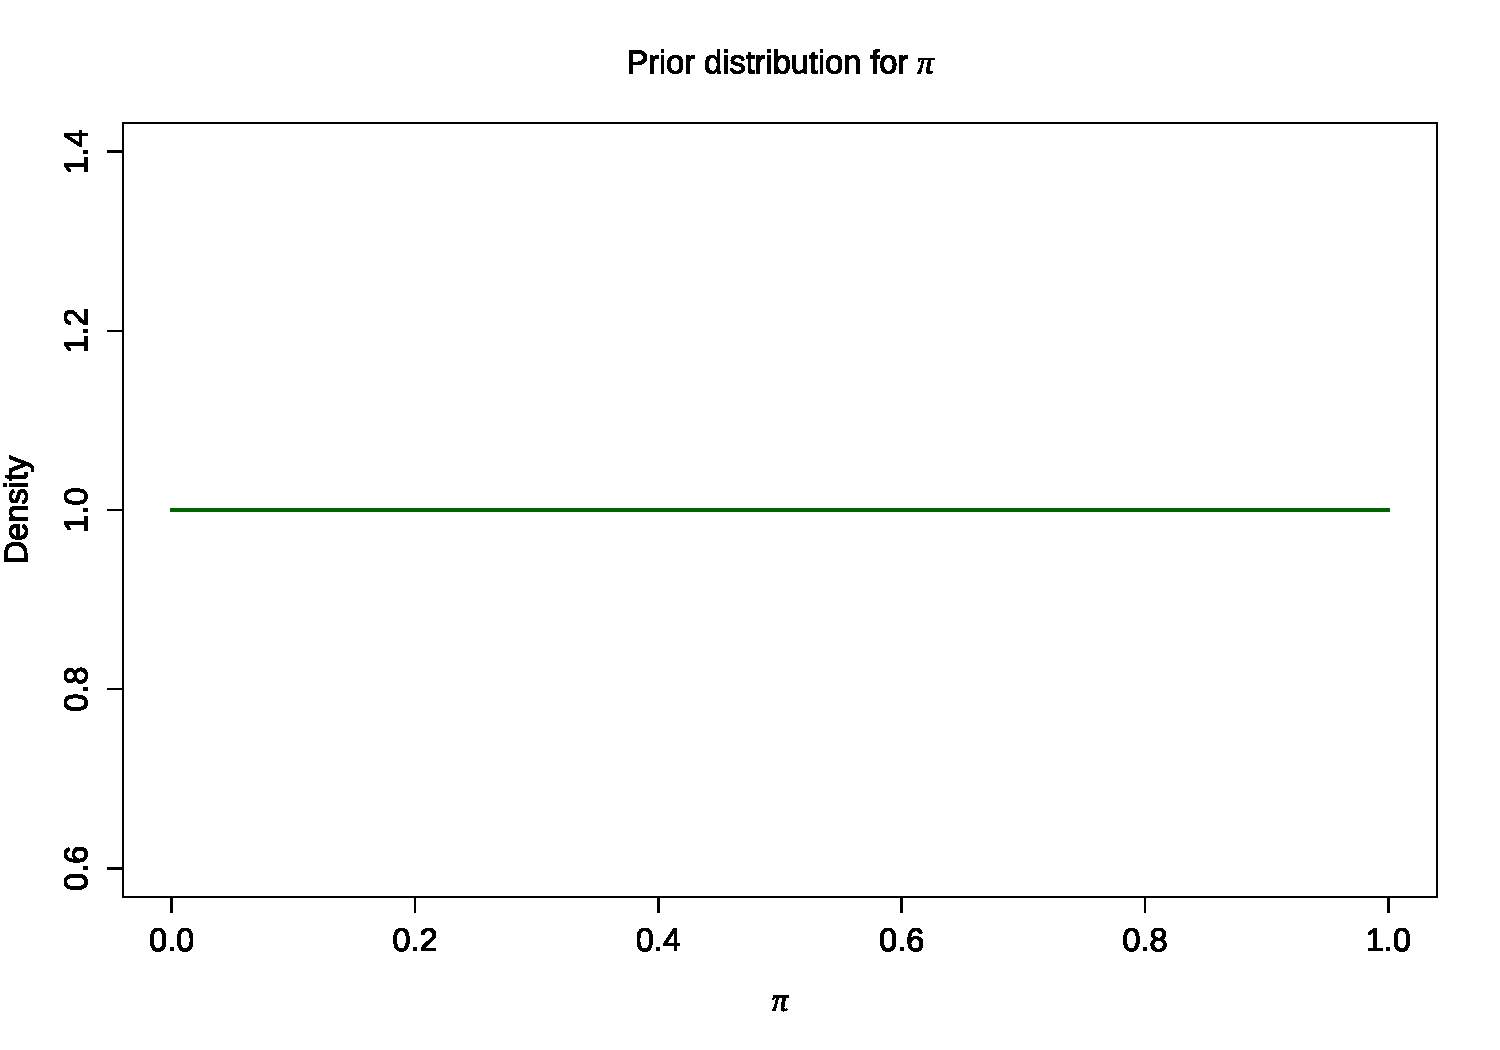
\includegraphics[keepaspectratio]{bayesian-glm_files/mediabag/bayesian-glm_files/figure-beamer/unnamed-chunk-58-1.pdf}}
\end{center}
\end{frame}

\begin{frame}{Calculating the Bayes Factor using the SDR}
\phantomsection\label{calculating-the-bayes-factor-using-the-sdr-2}
The ratio between the two black dots is the Bayes Factor.

\begin{center}
\pandocbounded{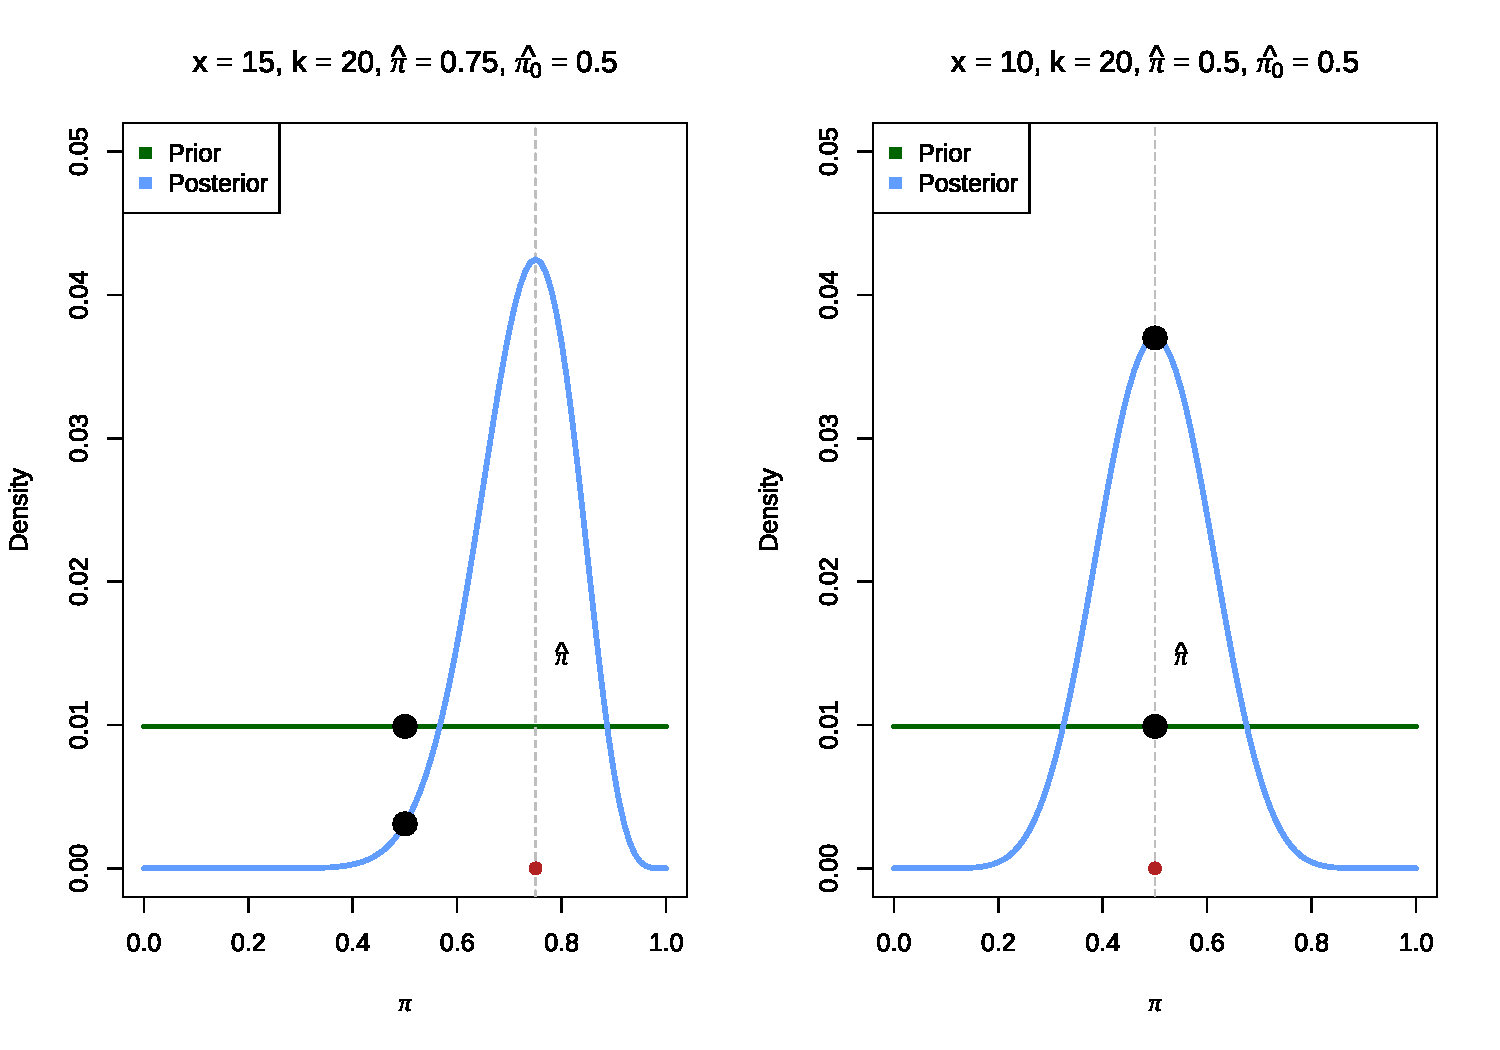
\includegraphics[keepaspectratio]{bayesian-glm_files/mediabag/bayesian-glm_files/figure-beamer/unnamed-chunk-59-1.pdf}}
\end{center}
\end{frame}

\begin{frame}{Bayes Factor in \texttt{brms}}
\phantomsection\label{bayes-factor-in-brms}
https://vuorre.com/posts/2017-03-21-bayes-factors-with-brms/
https://easystats.github.io/bayestestR/reference/bayesfactor\_parameters.html\#:\textasciitilde:text=For\%20the\%20computation\%20of\%20Bayes,flat\%20priors\%20the\%20null\%20is
\end{frame}

\begin{frame}[fragile]{Be careful with the Bayes Factor}
\phantomsection\label{be-careful-with-the-bayes-factor}
The Bayes Factor computed with \texttt{hypothesis()} or in general the
SDR method is highly sensitive to the priors. See also the
\texttt{bayestestR}
\href{https://easystats.github.io/bayestestR/reference/bayesfactor_parameters.html\#setting-the-correct-prior}{documentation}.
In general:

\begin{itemize}
\tightlist
\item
  The Bayes Factor requires informative or at least non-flat priors.
  Remember that in \texttt{brms} the default prior is flat
\item
  As the prior scale (e.g., standard deviation) increase, the Bayes
  Factor tends to suggest evidence for the null hypothesis, even when
  the null hypothesis is false
\end{itemize}

This is called
\href{https://en.wikipedia.org/wiki/Lindley\%27s_paradox}{Lindley's
paradox}. (see \citeproc{ref-Wagenmakers2023-ll}{Wagenmakers and Ly
2023}).
\end{frame}

\begin{frame}[fragile]{Lindley's paradox, a simulation}
\phantomsection\label{lindleys-paradox-a-simulation}
We can just simulate a t-test (or equivalently a parameter of a model)
and run the Bayesian model with different prior distribution scale.

For a t-test we are focused on the prior for the (standardized)
difference between the means. We can set a prior centered on 0 with
different scale.

Here I'm using the \texttt{BayesFactor} package just because is faster
for simple model if we are interested in the Bayes Factor pointnull (the
same as \texttt{brms::hypothesis(x,\ "b\ =\ 0")}).
\end{frame}

\begin{frame}{Lindley's paradox, a simulation}
\phantomsection\label{lindleys-paradox-a-simulation-1}
\begin{center}
\pandocbounded{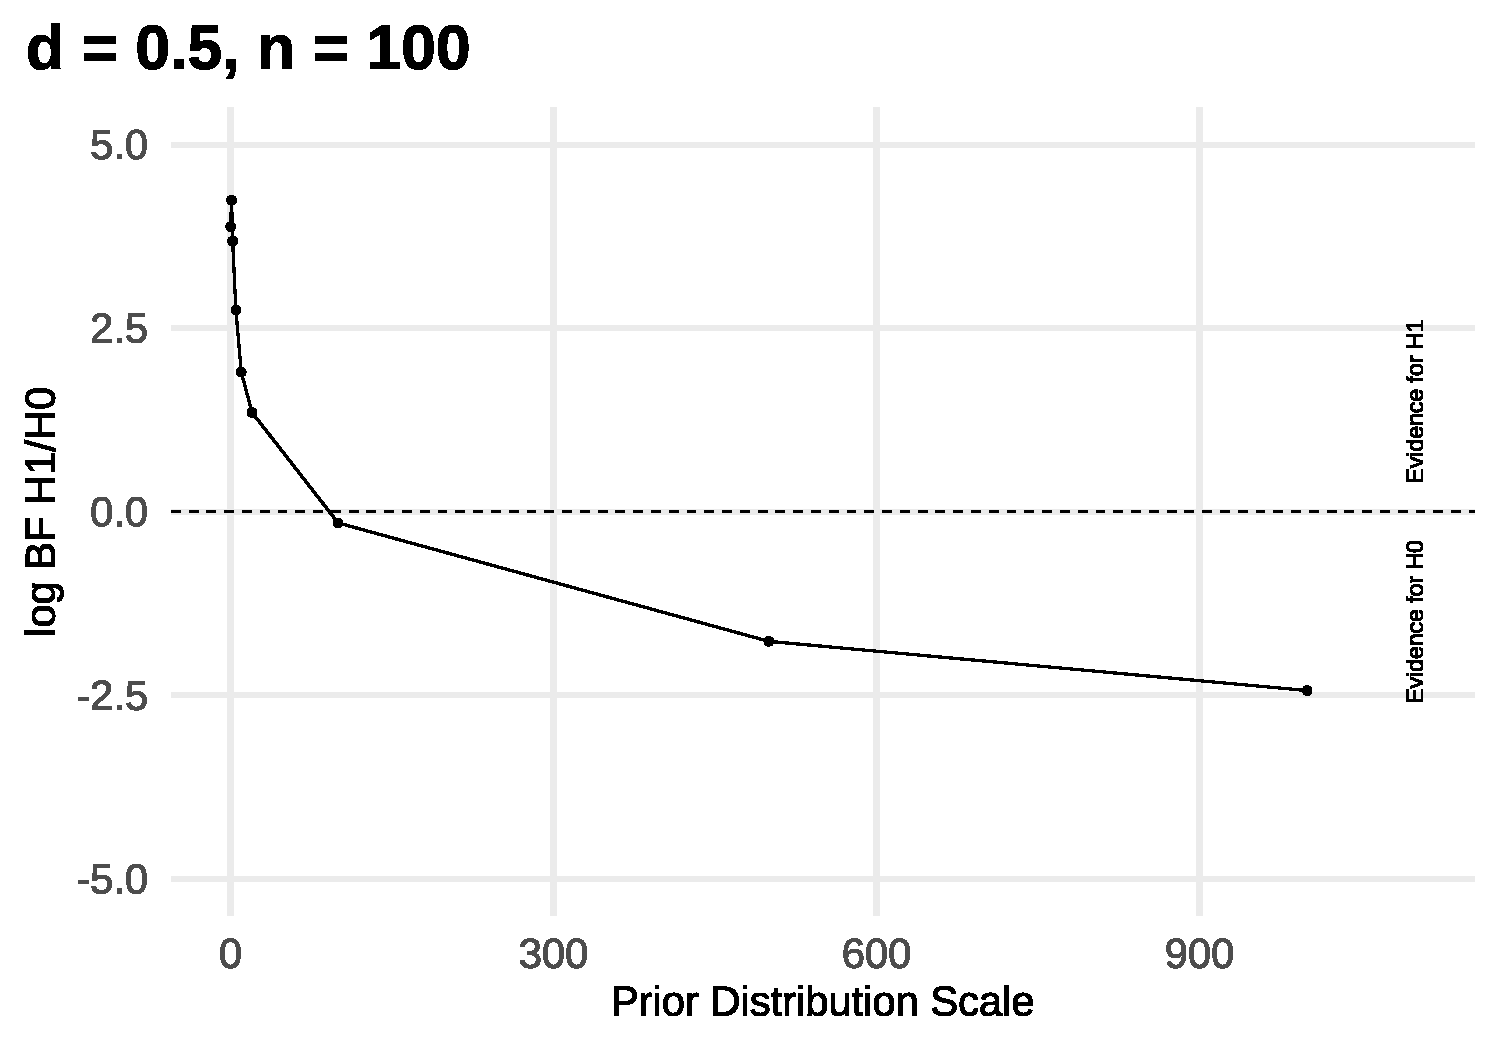
\includegraphics[keepaspectratio]{bayesian-glm_files/mediabag/bayesian-glm_files/figure-beamer/unnamed-chunk-60-1.pdf}}
\end{center}
\end{frame}

\begin{frame}{Prior Sensitivity Check}
\phantomsection\label{prior-sensitivity-check}
Given the sensitivity of Bayesian models to the prior, especially when
informative is always a good idea to check the actual impact of priors.
Not only for Bayes Factors but also for the posterior distributions.

\begin{itemize}
\tightlist
\item
  Run your model with the prior that are more plausible for you
\item
  Run the same model with priors that are more and less informative
\item
  Check the impact of the prior on your posterior distributions and
  conclusions
\end{itemize}
\end{frame}

\begin{frame}[fragile]{Prior Predictive Check}
\phantomsection\label{prior-predictive-check}
The prior predictive check is an important process when setting the
priors in a regression model. The basic idea is that the posterior
distribution is the combination between priors and likelihood (i.e., the
data). If we remove likelihood from the equation, we obtain a
``posterior'' only using information in the prior.

The advantage is that we can simulate data to check if our priors are
reasonable according to our model, phenomenon, etc.

In \texttt{brms} there is an argument called \texttt{sample\_prior} that
can be set to \texttt{"only"} to fit a model ignoring the data:

\begin{Shaded}
\begin{Highlighting}[]
\FunctionTok{brm}\NormalTok{(}
\NormalTok{  y }\SpecialCharTok{\textasciitilde{}}\NormalTok{ x,}
  \AttributeTok{data =}\NormalTok{ dat, }\CommentTok{\# not used}
  \AttributeTok{sample\_prior =} \StringTok{"only"}
\NormalTok{)}
\end{Highlighting}
\end{Shaded}
\end{frame}

\begin{frame}[fragile]{Prior predictive check}
\phantomsection\label{prior-predictive-check-1}
Assuming to have a simple model with a continous and categorical
predictor:

\begin{verbatim}
#>            y          x g
#> 1  0.7812706  0.6207567 0
#> 2 -1.1101886  0.0356414 0
#> 3  0.3243795  0.7731545 0
#> 4  1.8243161  1.2724891 0
#> 5  0.6446891  0.3709754 0
#> 6  1.0857640 -0.1628543 0
\end{verbatim}
\end{frame}

\begin{frame}[fragile]{Prior predictive check}
\phantomsection\label{prior-predictive-check-2}
We know that \texttt{x} and \texttt{y} are standandardized thus we can
think about the effect \texttt{g} in terms of Cohen's \(d\) and the
effect of \texttt{x} in terms of units of standard deviations. Let's set
some priors for \(\beta_1\) and \(\beta_2\).

\begin{Shaded}
\begin{Highlighting}[]
\FunctionTok{get\_prior}\NormalTok{(y }\SpecialCharTok{\textasciitilde{}}\NormalTok{ x }\SpecialCharTok{+}\NormalTok{ g, }\AttributeTok{data =}\NormalTok{ dat)}
\end{Highlighting}
\end{Shaded}

\begin{verbatim}
#>                 prior     class coef group resp dpar nlpar lb ub       source
#>                (flat)         b                                       default
#>                (flat)         b    g                             (vectorized)
#>                (flat)         b    x                             (vectorized)
#>  student_t(3, 0, 2.5) Intercept                                       default
#>  student_t(3, 0, 2.5)     sigma                             0         default
\end{verbatim}
\end{frame}

\begin{frame}[fragile]{Prior predictive check}
\phantomsection\label{prior-predictive-check-3}
\begin{Shaded}
\begin{Highlighting}[]
\NormalTok{priors }\OtherTok{\textless{}{-}} \FunctionTok{c}\NormalTok{(}
  \FunctionTok{prior}\NormalTok{(}\FunctionTok{normal}\NormalTok{(}\DecValTok{0}\NormalTok{, }\DecValTok{1}\NormalTok{), }\AttributeTok{class =} \StringTok{"b"}\NormalTok{, }\AttributeTok{coef =} \StringTok{"g"}\NormalTok{),}
  \FunctionTok{prior}\NormalTok{(}\FunctionTok{normal}\NormalTok{(}\DecValTok{0}\NormalTok{, }\DecValTok{2}\NormalTok{), }\AttributeTok{class =} \StringTok{"b"}\NormalTok{, }\AttributeTok{coef =} \StringTok{"x"}\NormalTok{)}
\NormalTok{)}

\NormalTok{fit\_prior }\OtherTok{\textless{}{-}} \FunctionTok{brm}\NormalTok{(y }\SpecialCharTok{\textasciitilde{}}\NormalTok{ x }\SpecialCharTok{+}\NormalTok{ g, }\AttributeTok{data =}\NormalTok{ dat, }\AttributeTok{sample\_prior =} \StringTok{"only"}\NormalTok{, }\AttributeTok{prior =}\NormalTok{ priors, }\AttributeTok{file =} \FunctionTok{here}\NormalTok{(}\StringTok{"slides"}\NormalTok{, }\StringTok{"objects"}\NormalTok{, }\StringTok{"fit\_prior.rds"}\NormalTok{))}
\FunctionTok{summary}\NormalTok{(fit\_prior)}
\end{Highlighting}
\end{Shaded}

\begin{verbatim}
#>  Family: gaussian 
#>   Links: mu = identity; sigma = identity 
#> Formula: y ~ x + g 
#>    Data: dat (Number of observations: 50) 
#>   Draws: 4 chains, each with iter = 2000; warmup = 1000; thin = 1;
#>          total post-warmup draws = 4000
#> 
#> Regression Coefficients:
#>           Estimate Est.Error l-95% CI u-95% CI Rhat Bulk_ESS Tail_ESS
#> Intercept     0.30      5.00    -8.67     8.82 1.00     2585     1590
#> x             0.03      2.04    -4.00     3.96 1.00     2844     2449
#> g            -0.02      1.00    -2.05     1.91 1.00     3089     2397
#> 
#> Further Distributional Parameters:
#>       Estimate Est.Error l-95% CI u-95% CI Rhat Bulk_ESS Tail_ESS
#> sigma     2.79      3.83     0.08    10.10 1.00     2647     1440
#> 
#> Draws were sampled using sampling(NUTS). For each parameter, Bulk_ESS
#> and Tail_ESS are effective sample size measures, and Rhat is the potential
#> scale reduction factor on split chains (at convergence, Rhat = 1).
\end{verbatim}
\end{frame}

\begin{frame}{Prior predictive check}
\phantomsection\label{prior-predictive-check-4}
\begin{center}
\pandocbounded{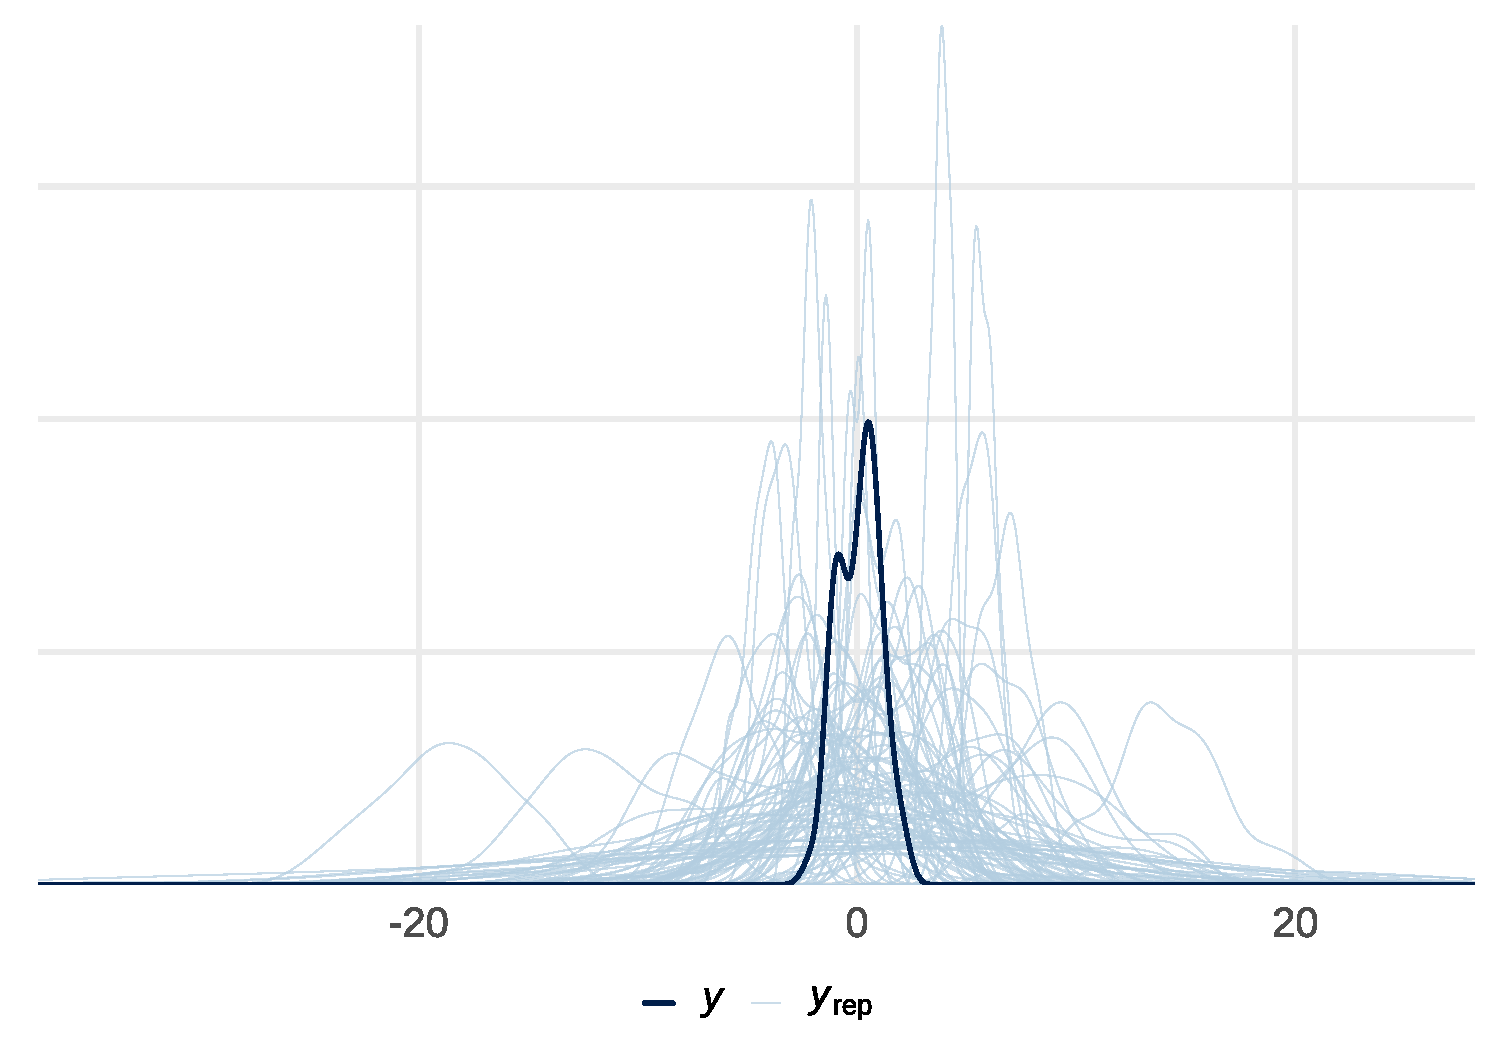
\includegraphics[keepaspectratio]{bayesian-glm_files/mediabag/bayesian-glm_files/figure-beamer/unnamed-chunk-65-1.pdf}}
\end{center}
\end{frame}

\begin{frame}[fragile]{Extracting Posterior Distributions}
\phantomsection\label{extracting-posterior-distributions}
When running a model with \texttt{lm} and \texttt{glm}, all the required
information is included into the summary of the model. For each
parameter we have the point estimate, standard error, confidence
interval, etc.

\begin{Shaded}
\begin{Highlighting}[]
\NormalTok{fit\_lm\_example }\OtherTok{\textless{}{-}} \FunctionTok{lm}\NormalTok{(Sepal.Length }\SpecialCharTok{\textasciitilde{}}\NormalTok{ Petal.Width }\SpecialCharTok{+}\NormalTok{ Species, }\AttributeTok{data =}\NormalTok{ iris)}
\FunctionTok{summary}\NormalTok{(fit\_lm\_example)}
\end{Highlighting}
\end{Shaded}

\begin{verbatim}
#> 
#> Call:
#> lm(formula = Sepal.Length ~ Petal.Width + Species, data = iris)
#> 
#> Residuals:
#>     Min      1Q  Median      3Q     Max 
#> -1.3891 -0.3043 -0.0472  0.2528  1.3358 
#> 
#> Coefficients:
#>                   Estimate Std. Error t value Pr(>|t|)    
#> (Intercept)        4.78044    0.08308  57.543  < 2e-16 ***
#> Petal.Width        0.91690    0.19386   4.730 5.25e-06 ***
#> Speciesversicolor -0.06025    0.23041  -0.262    0.794    
#> Speciesvirginica  -0.05009    0.35823  -0.140    0.889    
#> ---
#> Signif. codes:  0 '***' 0.001 '**' 0.01 '*' 0.05 '.' 0.1 ' ' 1
#> 
#> Residual standard error: 0.481 on 146 degrees of freedom
#> Multiple R-squared:  0.6694, Adjusted R-squared:  0.6626 
#> F-statistic: 98.53 on 3 and 146 DF,  p-value: < 2.2e-16
\end{verbatim}
\end{frame}

\begin{frame}{Extracting Posterior Distributions}
\phantomsection\label{extracting-posterior-distributions-1}
With Bayesian models we have posterior distributions that can be
summarised in different ways. There are several methods and packages to
work with posteriors:
\end{frame}

\begin{frame}[fragile]{Extracting Posterior Distributions}
\phantomsection\label{extracting-posterior-distributions-2}
With the \texttt{as\_draws\_df} we can extract all the samples from the
posterior distribution:

\begin{verbatim}
#> # A draws_df: 6 iterations, 1 chains, and 6 variables
#>   b_Intercept b_mark sigma Intercept lprior lp__
#> 1        -9.6   0.15   1.5       4.3   -3.4  -59
#> 2       -10.2   0.16   1.4       4.1   -3.3  -59
#> 3        -9.0   0.15   1.5       4.6   -3.4  -62
#> 4        -9.0   0.15   1.4       4.3   -3.4  -60
#> 5        -8.7   0.14   1.5       3.8   -3.4  -59
#> 6        -8.0   0.13   1.4       3.7   -3.3  -60
#> # ... hidden reserved variables {'.chain', '.iteration', '.draw'}
\end{verbatim}
\end{frame}

\begin{frame}[fragile]{Extracting Posterior Distributions}
\phantomsection\label{extracting-posterior-distributions-3}
\begin{Shaded}
\begin{Highlighting}[]
\FunctionTok{as\_draws\_df}\NormalTok{(fit\_mark) }\SpecialCharTok{|\textgreater{}} 
  \FunctionTok{select}\NormalTok{(}\FunctionTok{starts\_with}\NormalTok{(}\StringTok{"b"}\NormalTok{), sigma) }\SpecialCharTok{|\textgreater{}} 
\NormalTok{  posterior}\SpecialCharTok{::}\FunctionTok{summarise\_draws}\NormalTok{()}
\end{Highlighting}
\end{Shaded}

\begin{verbatim}
#> # A tibble: 3 x 10
#>   variable     mean median     sd    mad       q5    q95  rhat ess_bulk ess_tail
#>   <chr>       <dbl>  <dbl>  <dbl>  <dbl>    <dbl>  <dbl> <dbl>    <dbl>    <dbl>
#> 1 b_Interce~ -7.96  -7.98  2.10   2.05   -11.5    -4.49   1.00    3049.    2798.
#> 2 b_mark      0.133  0.133 0.0230 0.0227   0.0954  0.172  1.00    3064.    2776.
#> 3 sigma       1.63   1.60  0.217  0.211    1.32    2.03   1.00    2706.    2588.
\end{verbatim}
\end{frame}

\begin{frame}[fragile]{HPDI with \texttt{bayestestR}}
\phantomsection\label{hpdi-with-bayestestr}
The \texttt{bayestestR} contains a lot of functions to do inference and
post-processing on \texttt{brms} (and also other) models:

\begin{Shaded}
\begin{Highlighting}[]
\NormalTok{bayestestR}\SpecialCharTok{::}\FunctionTok{hdi}\NormalTok{(fit\_mark)}
\end{Highlighting}
\end{Shaded}

\begin{verbatim}
#> Highest Density Interval
#> 
#> Parameter   |         95% HDI
#> -----------------------------
#> (Intercept) | [-12.24, -3.92]
#> mark        | [  0.09,  0.18]
\end{verbatim}

\begin{Shaded}
\begin{Highlighting}[]
\FunctionTok{plot}\NormalTok{(bayestestR}\SpecialCharTok{::}\FunctionTok{hdi}\NormalTok{(fit\_mark))}
\end{Highlighting}
\end{Shaded}

\begin{center}
\pandocbounded{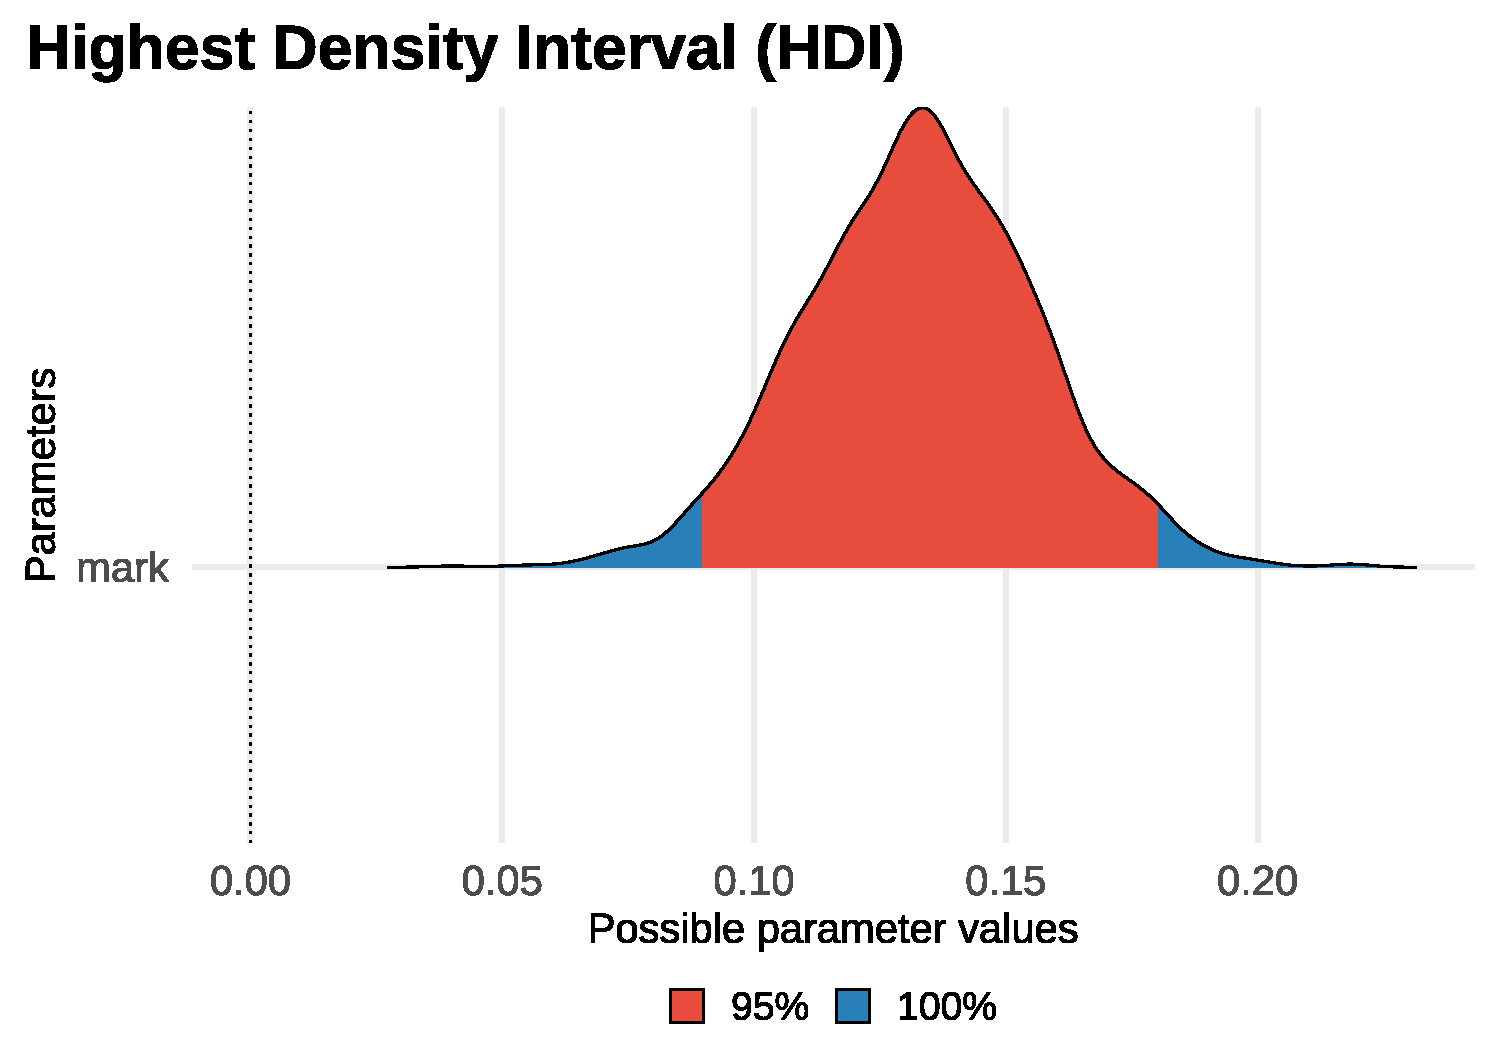
\includegraphics[keepaspectratio]{bayesian-glm_files/mediabag/bayesian-glm_files/figure-beamer/unnamed-chunk-70-1.pdf}}
\end{center}
\end{frame}

\begin{frame}[fragile]{The \texttt{broom} package}
\phantomsection\label{the-broom-package}
The \texttt{broom.mixed} package automatically provide the
\texttt{summary()} into a data.frame format:

\begin{Shaded}
\begin{Highlighting}[]
\FunctionTok{library}\NormalTok{(broom.mixed)}
\NormalTok{broom.mixed}\SpecialCharTok{::}\FunctionTok{tidy}\NormalTok{(fit\_mark)}
\end{Highlighting}
\end{Shaded}

\begin{verbatim}
#> # A tibble: 3 x 8
#>   effect   component group    term         estimate std.error conf.low conf.high
#>   <chr>    <chr>     <chr>    <chr>           <dbl>     <dbl>    <dbl>     <dbl>
#> 1 fixed    cond      <NA>     (Intercept)    -7.96     2.10   -12.2       -3.85 
#> 2 fixed    cond      <NA>     mark            0.133    0.0230   0.0882     0.179
#> 3 ran_pars cond      Residual sd__Observa~    1.63     0.217    1.27       2.11
\end{verbatim}
\end{frame}

\begin{frame}[fragile]{More on \texttt{bayestestR}}
\phantomsection\label{more-on-bayestestr}
This is a really amazing package, have a look at the \texttt{Features}
section because contains functions and explanations about different ways
of summarizing the posterior distribution.
\end{frame}

\begin{frame}{Packages}
\phantomsection\label{packages}
\end{frame}

\begin{frame}{References}
\phantomsection\label{references}
\phantomsection\label{refs}
\begin{CSLReferences}{1}{0}
\bibitem[\citeproctext]{ref-Gelman2019-hp}
Gelman, Andrew, Ben Goodrich, Jonah Gabry, and Aki Vehtari. 2019.
{``R-Squared for Bayesian Regression Models.''} \emph{The American
Statistician} 73: 307--9.
\url{https://doi.org/10.1080/00031305.2018.1549100}.

\bibitem[\citeproctext]{ref-Granziol2025-sy}
Granziol, Umberto, Maximilian Rabe, Marcello Gallucci, Andrea Spoto, and
Giulio Vidotto. 2025. {``Not Another Post Hoc Paper: A New Look at
Contrast Analysis and Planned Comparisons.''} \emph{Advances in Methods
and Practices in Psychological Science} 8 (January).
\url{https://doi.org/10.1177/25152459241293110}.

\bibitem[\citeproctext]{ref-Schad2020-ht}
Schad, Daniel J, Shravan Vasishth, Sven Hohenstein, and Reinhold Kliegl.
2020. {``How to Capitalize on a Priori Contrasts in Linear (Mixed)
Models: A Tutorial.''} \emph{Journal of Memory and Language} 110
(February): 104038. \url{https://doi.org/10.1016/j.jml.2019.104038}.

\bibitem[\citeproctext]{ref-Wagenmakers2010-fj}
Wagenmakers, Eric-Jan, Tom Lodewyckx, Himanshu Kuriyal, and Raoul
Grasman. 2010. {``Bayesian Hypothesis Testing for Psychologists: A
Tutorial on the Savage--Dickey Method.''} \emph{Cognitive Psychology} 60
(May): 158--89. \url{https://doi.org/10.1016/j.cogpsych.2009.12.001}.

\bibitem[\citeproctext]{ref-Wagenmakers2023-ll}
Wagenmakers, Eric-Jan, and Alexander Ly. 2023. {``History and Nature of
the Jeffreys-Lindley Paradox.''} \emph{Archive for History of Exact
Sciences} 77: 25--72. \url{https://doi.org/10.1007/s00407-022-00298-3}.

\end{CSLReferences}
\end{frame}




\end{document}
